\documentclass{Class/project_report}
\setTHSarabunFont
\geometry{a4paper,top=1.5in,bottom=1in,left=1.5in,right=1in}
\pagestyle{plain} % ตั้งค่า pagestyle เริ่มต้น
\newcolumntype{L}{>{\RaggedRight\arraybackslash}X} 
\begin{document}

    % Setup for Figures (centered label and text)
    \captionsetup[figure]{
      font={normalsize},
      labelfont={bold16pt},
      labelsep=quad,
      justification=centering,
      singlelinecheck=false,
      name={ภาพที่} % Add this line
    }
    % Setup for Tables (raggedright label and text)
    \captionsetup[table]{
      font={normalsize},
      labelfont={bold16pt},
      labelsep=quad,
      justification=raggedright,
      singlelinecheck=false,
      name={ตารางที่} % Add this line
    }
    %*************************************
% ปกนอก
%*************************************
\newpage
\thispagestyle{empty}
\begin{center}


\includegraphics[width=5.08cm]{Image/Logo_KMUTNB_Thai.png}
\vspace{2mm}

{\bf
    เว็บแอปพลิเคชันเพื่อการคอนฟิกด้วยวิธี NETCONF ผ่าน LLM     %ชื่อโปรเจ็คภาษาไทย
}

% กรณีทำโปรเจ็คคนเดียว 
\vspace{60mm}
{\bf
    นางชัยสิทธิ์ มินทกร %ชื่อผู้จัดทำ
}
\vspace{64mm}   


% กรณีมีเพื่อนร่วมทำโปรเจ็ค
%\vspace{56mm}
%{\bf
%    นางสาวสุพาภรณ์ ซิ้มเจริญ    %ชื่อผู้จัดทำ1
%    \\
%    นางสาวสิวาลัย จินเจือ       %ชื่อผู้จัดทำ2
%}
%\vspace{60mm}  




{\bf 
    %----------------------------------------------------
    % กรณีเป็นนักศึกษาหลักสูตร IT
    ปริญญานิพนธ์นี้เป็นส่วนหนึ่งของการศึกษาตามหลักสูตรวิทยาศาสตรบัณฑิต\\
    สาขาวิชาวิศวกรรมสารสนเทศและเครือข่าย ภาควิชาเทคโนโลยีสารสนเทศ\\
    
    % กรณีเป็นนักศึกษาหลักสูตร ITI
    %ปริญญานิพนธ์นี้เป็นส่วนหนึ่งของการศึกษาตามหลักสูตรอุตสาหกรรมศาสตรบัณฑิต\\
    %สาขาวิชาเทคโนโลยีสารสนเทศ (ต่อเนื่อง) ภาควิชาเทคโนโลยีสารสนเทศ\\
    
    % กรณีเป็นนักศึกษาหลักสูตร INE และ INET
    %ปริญญานิพนธ์นี้เป็นส่วนหนึ่งของการศึกษาตามหลักสูตรวิศวกรรมศาสตรบัณฑิต\\
    %สาขาวิชาวิศวกรรมสารสนเทศและเครือข่าย ภาควิชาเทคโนโลยีสารสนเทศ\\
    
    %----------------------------------------------------
    คณะเทคโนโลยีและการจัดการอุตสาหกรรม มหาวิทยาลัยเทคโนโลยีพระจอมเกล้าพระนครเหนือ    \\
    ปีการศึกษา 2568\\
    ลิขสิทธิ์ของมหาวิทยาลัยเทคโนโลยีพระจอมเกล้าพระนครเหนือ
}

\end{center}

%*************************************
% ปกในภาษาไทย
%*************************************
\newpage
\thispagestyle{empty}
\begin{center}


เว็บแอปพลิเคชันเพื่อการคอนฟิกด้วยวิธี NETCONF ผ่าน LLM      %ชื่อโปรเจ็คภาษาไทย

%----------------------------------------------------

% กรณีทำโปรเจ็คคนเดียว 
\vspace{90mm}
นางชัยสิทธิ์ มินทกร %ชื่อผู้จัดทำ
\vspace{94mm}   


% กรณีมีเพื่อนร่วมทำโปรเจ็ค
%\vspace{86mm}
%นางสาวสุพาภรณ์ ซิ้มเจริญ    %ชื่อผู้จัดทำ1
%\\
%นางสาวสิวาลัย จินเจือ       %ชื่อผู้จัดทำ2
%\vspace{90mm}  

%----------------------------------------------------
% กรณีเป็นนักศึกษาหลักสูตร IT
ปริญญานิพนธ์นี้เป็นส่วนหนึ่งของการศึกษาตามหลักสูตรวิทยาศาสตรบัณฑิต\\
สาขาวิชาวิศวกรรมสารสนเทศและเครือข่าย ภาควิชาเทคโนโลยีสารสนเทศ\\

% กรณีเป็นนักศึกษาหลักสูตร ITI
%ปริญญานิพนธ์นี้เป็นส่วนหนึ่งของการศึกษาตามหลักสูตรอุตสาหกรรมศาสตรบัณฑิต\\
%สาขาวิชาเทคโนโลยีสารสนเทศ (ต่อเนื่อง) ภาควิชาเทคโนโลยีสารสนเทศ\\

% กรณีเป็นนักศึกษาหลักสูตร INE และ INET
%ปริญญานิพนธ์นี้เป็นส่วนหนึ่งของการศึกษาตามหลักสูตรวิศวกรรมศาสตรบัณฑิต\\
%สาขาวิชาวิศวกรรมสารสนเทศและเครือข่าย ภาควิชาเทคโนโลยีสารสนเทศ\\

%----------------------------------------------------
คณะเทคโนโลยีและการจัดการอุตสาหกรรม มหาวิทยาลัยเทคโนโลยีพระจอมเกล้าพระนครเหนือ\\
ปีการศึกษา 2568\\
ลิขสิทธิ์ของมหาวิทยาลัยเทคโนโลยีพระจอมเกล้าพระนครเหนือ

\end{center}


%*************************************
% ปกในภาษาอังกฤษ
%*************************************
\newpage
\thispagestyle{empty}
\begin{center}


Web Application for NETCONF Configuration via LLM      %ชื่อโปรเจ็คภาษาอังกฤษ


% กรณีทำโปรเจ็คคนเดียว 
\vspace{80mm}
MR.CHAIYASIT MINTAKORN      %ชื่อผู้จัดทำ
\vspace{84mm}   


% กรณีมีเพื่อนร่วมทำโปรเจ็ค
%\vspace{76mm}
%MS.SUPAPORN SIMCHAROEN       %ชื่อผู้จัดทำ1
%\\
%MS.SIWALAI CHINCHUA          %ชื่อผู้จัดทำ2
%\vspace{80mm}  



PROJECT REPORT SUBMITTED IN PARTIAL FULFILLMENT OF THE REQUIREMENTS\\
%----------------------------------------------------

% กรณีเป็นนักศึกษาหลักสูตร IT
FOR THE BACHELOR’S DEGREE OF SCIENCE\\
PROGRAM IN INFORMATION AND NETWORK ENGINEERING\\

% กรณีเป็นนักศึกษาหลักสูตร ITI
%FOR THE BACHELOR’S DEGREE OF INDUSTRIAL TECHNOLOGY\\ 
%PROGRAM IN INFORMATION TECHNOLOGY (CONTINUING PROGRAM)\\

% กรณีเป็นนักศึกษาหลักสูตร INE และ INET
%FOR THE BACHELOR’S DEGREE OF ENGINEERING\\
%PROGRAM IN INFORMATION AND NETWORK ENGINEERING\\

%----------------------------------------------------
DEPARTMENT OF INFORMATION TECHNOLOGY\\
FACULTY OF INDUSTRIAL TECHNOLOGY AND MANAGEMENT\\
KING MONGKUT’S UNIVERSITY OF TECHNOLOGY NORTH BANGKOK\\
ACADEMIC YEAR 2025\\
COPYRIGHT OF KING MONGKUT’S UNIVERSITY OF TECHNOLOGY NORTH BANGKOK

\end{center}

    
    %**************************************************************************************
% ใบรับรองโครงงาน กรณี ไม่มี ที่ปรึกษาร่วม
%**************************************************************************************
\newpage
\thispagestyle{empty}
\setstretch{1.25}
\setlength{\parindent}{0pt}

\begin{tcolorbox}[colframe=black, colback=white, width=\textwidth, boxrule=0.8pt, arc=1mm, auto outer arc, left=10pt, right=10pt, top=10pt, bottom=10pt, enhanced jigsaw]

\begin{center}
\vspace{3mm}

\includegraphics[width=3.18cm]{Image/Logo_KMUTNB_Thai.png}

{\bf {\fontTwentyFour
    ใบรับรองปริญญานิพนธ์
    \\
}{\fontEighteen
    คณะเทคโนโลยีและการจัดการอุตสาหกรรม
    \\
    มหาวิทยาลัยเทคโนโลยีพระจอมเกล้าพระนครเหนือ
}}
\end{center}
\vspace{1em}
\fontSixTeen{
\begin{tabbing}
    เรื่อง  \= การเขียนเล่มปริญญานิพนธ์ด้วย LaTeX       %ชื่อโปรเจ็คภาษาไทย
    \\
    โดย  \> นางสาวสุพาภรณ์ ซิ้มเจริญ     %ชื่อผู้จัดทำ1 
    %\\     %เว้นบรรทัด เมื่อมีเพื่อนร่วมโปรเจ็ค
        %\> นางสาวสิวาลัย จินเจือ       %ชื่อผู้จัดทำ2
    \\
    \\
         \> ได้รับอนุมัติให้นับเป็นส่วนหนึ่งของการศึกษาตาม 
    \\
         \> หลักสูตรวิทยาศาสตรบัณฑิต  สาขาวิชาเทคโนโลยีสารสนเทศ % กรณีเป็นนักศึกษาหลักสูตร IT
         %\> หลักสูตรอุตสาหกรรมศาสตรบัณฑิต  สาขาวิชาเทคโนโลยีสารสนเทศ (ต่อเนื่อง) % กรณีเป็นนักศึกษาหลักสูตร ITI
         %\> หลักสูตรวิศวกรรมศาสตรบัณฑิต  สาขาวิชาวิศวกรรมสารสนเทศและเครือข่าย % กรณีเป็นนักศึกษาหลักสูตร INE และ INET
      
\end{tabbing}

\vspace{1.5em}

\begin{flushright}
\makebox[8cm][l]{\rule{7cm}{0.4pt} คณบดี} \\
\makebox[8cm][l]{(ผู้ช่วยศาสตราจารย์ ดร.กฤษฎากร  บุดดาจันทร์)}
\end{flushright}


\vspace{14mm}  %กรณีทำโปรเจ็คคนเดียว
%\vspace{8mm}  %กรณีมีเพื่อนร่วมโปรเจ็ค



คณะกรรมการสอบโครงงานสหกิจศึกษา

\vspace{1.5em}
\begin{flushleft}
\makebox[7cm][l]{\rule{7cm}{0.4pt} ประธานกรรมการ} \\
\makebox[7cm][c]{(ผู้ช่วยศาสตาจารย์ ดร.บีสุดา ดาวเรือง)}       %ระบุชื่อประธานกรรมการ
\end{flushleft}

\vspace{1.5em}
\begin{flushleft}
\makebox[7cm][l]{\rule{7cm}{0.4pt} กรรมการ} \\
\makebox[7cm][c]{(อาจารย์ ดร.กาญจน์ ณ ศรีธะ)}            %ระบุชื่อกรรมการ
\end{flushleft}

\vspace{1.5em}
\begin{flushleft}
\makebox[7cm][l]{\rule{7cm}{0.4pt} กรรมการ} \\
\makebox[7cm][c]{(รองศาสตราจารย์ ดร.อนิราช มิ่งขวัญ)}       %ระบุชื่ออาจารย์ที่ปรึกษาโปรเจ็ค
\end{flushleft}

} %end fontSixTeen
\end{tcolorbox}
 %กรณี ไม่มี ที่ปรึกษาร่วม
    %%**************************************************************************************
% ใบรับรองโครงงาน กรณี มี ที่ปรึกษาร่วม
%**************************************************************************************
\newpage
\thispagestyle{empty}
\setstretch{1.25}
\setlength{\parindent}{0pt}

\begin{tcolorbox}[colframe=black, colback=white, width=\textwidth, boxrule=0.8pt, arc=1mm, auto outer arc, left=10pt, right=10pt, top=10pt, bottom=10pt, enhanced jigsaw]

\begin{center}
\vspace{3mm}

\includegraphics[width=3.18cm]{Image/Logo_KMUTNB_Thai.png}

{\bf {\fontTwentyFour
    ใบรับรองปริญญานิพนธ์
    \\
}{\fontEighteen
    คณะเทคโนโลยีและการจัดการอุตสาหกรรม
    \\
    มหาวิทยาลัยเทคโนโลยีพระจอมเกล้าพระนครเหนือ
}}
\end{center}
\vspace{1em}
\fontSixTeen{
\begin{tabbing}
    เรื่อง  \= การเขียนเล่มปริญญานิพนธ์ด้วย LaTeX       %ชื่อโปรเจ็คภาษาไทย
    \\
    โดย  \> นางสาวสุพาภรณ์ ซิ้มเจริญ     %ชื่อผู้จัดทำ1 
    \\     %เว้นบรรทัด เมื่อมีเพื่อนร่วมโปรเจ็ค
        \> นางสาวสิวาลัย จินเจือ       %ชื่อผู้จัดทำ2
    \\
    \\
         \> ได้รับอนุมัติให้นับเป็นส่วนหนึ่งของการศึกษาตาม 
    \\
         \> หลักสูตรวิทยาศาสตรบัณฑิต  สาขาวิชาเทคโนโลยีสารสนเทศ
\end{tabbing}

\vspace{1em}

\begin{flushright}
\makebox[8cm][l]{\rule{7cm}{0.4pt} คณบดี} \\
\makebox[8cm][l]{(ผู้ช่วยศาสตราจารย์ ดร.กฤษฎากร  บุดดาจันทร์)}
\end{flushright}


%\vspace{14mm}  %กรณีทำโปรเจ็คคนเดียว
\vspace{0.9em}  %กรณีมีเพื่อนร่วมโปรเจ็ค



คณะกรรมการสอบโครงงานสหกิจศึกษา

\vspace{0.9em}
\begin{flushleft}
\makebox[7cm][l]{\rule{7cm}{0.4pt} ประธานกรรมการ} \\
\makebox[7cm][c]{(ผู้ช่วยศาสตาจารย์ ดร.บีสุดา ดาวเรือง)}       %ระบุชื่อประธานกรรมการ
\end{flushleft}

\vspace{0.9em}
\begin{flushleft}
\makebox[7cm][l]{\rule{7cm}{0.4pt} กรรมการ} \\
\makebox[7cm][c]{(อาจารย์ ดร.กาญจน์ ณ ศรีธะ)}            %ระบุชื่อกรรมการ
\end{flushleft}

\vspace{0.9em}
\begin{flushleft}
\makebox[7cm][l]{\rule{7cm}{0.4pt} กรรมการ} \\
\makebox[7cm][c]{(รองศาสตราจารย์ ดร.อนิราช มิ่งขวัญ)}       %ระบุชื่ออาจารย์ที่ปรึกษาโปรเจ็ค
\end{flushleft}

\vspace{0.9em}
\begin{flushleft}
\makebox[7cm][l]{\rule{7cm}{0.4pt} ที่ปรึกษาร่วม} \\
\makebox[7cm][c]{(ผู้ช่วยศาสตาจารย์ ดร.นิติการ นาคเจือทอง)}       %ระบุชื่อที่ปรึกษาร่วม
\end{flushleft}


} %end fontSixTeen
\end{tcolorbox}
 %กรณี มี ที่ปรึกษาร่วม

    
    \newpage
    \thaiPageStyle
    \setcounter{page}{1}
    \fontSixTeen
    \justifying
    %**************************************************************************************
% บทคัดย่อภาษาไทย
%**************************************************************************************
\phantomsection
\addcontentsline{toc}{chapter}{บทคัดย่อภาษาไทย}
\begin{tabularx}{\textwidth}{lX}
ชื่อ                           & : นายชัยสิทธิ์ มินทกร         %ชื่อผู้จัดทำ1
%\\     %เว้นบรรทัด เมื่อมีเพื่อนร่วมโปรเจ็ค
%                             & : นางสาวสิวาลัย จินเจือ            %ชื่อผู้จัดทำ2 
\\
ชื่อปริญญานิพนธ์                  & : \hangindent=0.5em          % มีไว้สำหรับตอนชื่อโปรเจ็คเกิน 1 บรรทัด
                                เว็บแอปพลิเคชันเพื่อการคอนฟิกด้วยวิธี NETCONF ผ่าน LLM
\\
สาขาวิชา                       & : วิศวกรรมสารสนเทศและเครือข่าย % กรณีเป็นนักศึกษาหลักสูตร IT
%สาขาวิชา                       & : เทคโนโลยีสารสนเทศ (ต่อเนื่อง) % กรณีเป็นนักศึกษาหลักสูตร ITI
%สาขาวิชา                       & : วิศวกรรมสารสนเทศและเครือข่าย % กรณีเป็นนักศึกษาหลักสูตร INE และ INET
\\
                             & : มหาวิทยาลัยเทคโนโลยีพระจอมเกล้าพระนครเหนือ
\\
อาจารย์ที่ปรึกษาปริญญานิพนธ์        & : อาจารย์ ดร.วัชรชัย คงศิริวัฒนา   %ระบุชื่ออาจารย์ที่ปรึกษา
%\\      %เว้นบรรทัด เมื่อมีที่ปรึกษาร่วม
%ที่ปรึกษาร่วม                    & : ผู้ช่วยศาสตาจารย์ ดร.นิติการ นาคเจือทอง    %ระบุชื่อที่ปรึกษาร่วม (ถ้ามี)
\\
ปีการศึกษา                     & : 2568     %ระบุปีการศึกษา
\end{tabularx}

\vspace{5mm}
\phantomsection
\begin{center}\textbf{บทคัดย่อ}\end{center}
\hspace*{1.5em} %ย่อหน้า
โครงการนี้มีวัตถุประสงค์ในการพัฒนาเว็บแอปพลิเคชันเพื่อการจัดการเครือข่าย ที่ช่วยให้ผู้ดูแลระบบสามารถดำเนินการตั้งค่าอุปกรณ์เครือข่าย Cisco ได้อย่างมีประสิทธิภาพและสะดวกยิ่งขึ้น ระบบที่พัฒนาขึ้นรองรับการกำหนดค่าพื้นฐาน เช่น การตั้งค่า IP Address การกำหนดค่า VLAN และการจัดการ Routing Protocols โดยใช้ Node.js และ Express สำหรับการพัฒนา Backend และ React สำหรับการพัฒนา Frontend พร้อมทั้งเชื่อมต่อกับ MongoDB เพื่อจัดเก็บข้อมูลอุปกรณ์

\hspace*{1.5em} %ย่อหน้า
นอกจากนี้ ระบบยังผสานเทคโนโลยี Large Language Model (LLM) เพื่อสร้างการกำหนดค่าอัตโนมัติจาก Prompt ที่ผู้ใช้กรอก ช่วยลดความซับซ้อนและความผิดพลาดในการกำหนดค่าด้วยตนเอง อีกทั้งยังมีความสามารถในการ สำรองข้อมูล (Backup) และ กู้คืนการตั้งค่า (Rollback) ของอุปกรณ์เพื่อรองรับการจัดการอย่างปลอดภัย

\hspace*{1.5em} %ย่อหน้า
ผลลัพธ์ที่ได้จากโครงการช่วยเพิ่มประสิทธิภาพในการจัดการเครือข่าย ลดระยะเวลาในการกำหนดค่า และเพิ่มความยืดหยุ่นในการดูแลรักษาอุปกรณ์เครือข่าย Cisco ให้มีความทันสมัยและสอดคล้องกับความต้องการขององค์กรในยุคดิจิทัล
\begin{flushright}
(ปริญญานิพนธ์มีจำนวนทั้งสิ้น \pageref{LastPage} หน้า)

\vfill
\rule{10 cm}{0.4pt} อาจารย์ที่ปรึกษาปริญญานิพนธ์ 
%\\ \vspace{3mm}                        %เว้นกรณีมีที่ปรึกษาร่วม
%\rule{12.6 cm}{0.4pt} ที่ปรึกษาร่วม         % กรณีมีที่ปรึกษาร่วม

\end{flushright}





%**************************************************************************************
% บทคัดย่อภาษาอังกฤษ
%**************************************************************************************
\newpage
\phantomsection
\addcontentsline{toc}{chapter}{บทคัดย่อภาษาอังกฤษ}
\begin{tabularx}{\textwidth}{lX}
Name                    & : MR.CHAIYASIT MINTAKORN  %ชื่อผู้จัดทำ1
%\\      %เว้นบรรทัดเมื่อมีเพื่อนร่วมโปรเจ็ค
%                       & : Ms.Siwalai Chinchua      %ชื่อผู้จัดทำ2
\\
Project Title           & : \hangindent=0.5em % มีไว้สำหรับตอนชื่อโปรเจ็คเกิน 1 บรรทัด
                            Web Application for NETCONF Configuration via LLM  %ระบุชื่อโปรเจ็คภาษาอังกฤษ
\\
Major Field             & : Information and Network Engineering % กรณีเป็นนักศึกษาหลักสูตร IT
%Major Field             & : Information Technology (Continuing Program) % กรณีเป็นนักศึกษาหลักสูตร ITI
%Major Field             & : Information and Network Engineering % กรณีเป็นนักศึกษาหลักสูตร INE และ INET
\\
                        & : King Mongkut’s University of Technology North Bangkok
\\
Project Advisor         & : Dr.Watcharachai Kongsiriwattana  %ระบุชื่ออาจารย์ที่ปรึกษา
%\\      %เว้นบรรทัด เมื่อมีที่ปรึกษาร่วม
%Co-Advisor              & : Asst. Prof. Dr.Nitigan Nakjuatong   %ระบุชื่อที่ปรึกษาร่วม (ถ้ามี)
\\
Academic Year           & : 2025    %ระบุปีการศึกษา
\end{tabularx}

\vspace{5mm}
\begin{center}\textbf{Abstract}\end{center}

\hspace*{1.5em} %ย่อหน้า
This project, "Writing a Project Report with LaTeX," aims to present practical guidelines for preparing a complete thesis document, from the cover page to the appendices. It utilizes the LaTeX document processing system, widely accepted in academic circles due to its efficient handling of complex documents and precise, standardized formatting. Therefore, LaTeX is considered an essential tool for students, facilitating a more effective and streamlined thesis preparation process. The content covers key components of a thesis, beginning with the Thai Abstract, English Abstract, Acknowledgments, Table of Contents, List of Figures, List of Tables, Chapter 1: Introduction, Chapter 2: Concepts, Theories, and Related Research, Chapter 3: Methodology, Chapter 4: Results, Chapter 5: Conclusion, and Bibliography, including Appendices. Additionally, emphasis is placed on the correct and systematic insertion of figures and tables, as well as the management of in-text citations.

\begin{flushright}
(Total \pageref{LastPage} pages)

\vfill

\rule{12 cm}{0.4pt} Project Advisor
%\\ \vspace{3mm}                          %เว้นกรณีมีที่ปรึกษาร่วม
%\rule{12.7 cm}{0.4pt} Co-Advisor         % กรณีมีที่ปรึกษาร่วม

\end{flushright}


%**************************************************************************************
% กิตติกรรมประกาศ
%**************************************************************************************
\newpage
\phantomsection
\addcontentsline{toc}{chapter}{กิตติกรรมประกาศ}
\begin{center}\textbf{กิตติกรรมประกาศ}\end{center}

\hspace*{1.5em}  %ย่อหน้า
ปริญานิพนธ์ "เว็บแอปพลิเคชันเพื่อการคอนฟิกด้วยวิธี NETCONF ผ่าน LLM" จะไม่สามารถสำเร็จลุล่วงไปได้ด้วยดีหากไม่ได้รับการช่วยเหลือและความอนุเคราะห์จากบุคคลหลายท่าน ทางผู้จัดทำต้องขอขอบพระคุณ รองศาสตราจารย์ ดร.อนิราช มิ่งขวัญ ซึ่งเป็นอาจารย์ที่ปรึกษา ที่ได้กรุณาให้คำปรึกษา และแนะนำแนวทางในการจัดทำปริญญานิพนธ์ รวมทั้งคณาจารย์ภาควิชาเทคโนโลยีสารสนเทศที่ได้ให้ความรู้กับผู้จัดทำเพื่อนำมาประยุกต์ในการจัดทำปริญญานิพนธ์นี้
\\
\hspace*{1.5em}  %ย่อหน้า
ท้ายที่สุดนี้ ทางผู้จัดทำขอน้อมรำลึกพระคุณบิดา มารดา ผู้ซึ่งมีพระคุณอย่างสูงสุดที่ให้ความอุปการะผู้จัดทำมาโดยตลอด รวมทั้งผู้มีพระคุณทุกท่าน คณะผู้จัดทำรู้สึกซาบซึ้งเป็นอย่างยิ่ง จึงใคร่ขอขอบพระคุณเป็นอย่างสูงมา ณ โอกาสนี้ด้วย
\\
\begin{flushright}
\makebox[6cm][l]{ชัยสิทธิ์ มินทกร}      %ชื่อผู้จัดทำ1
%\\     %เว้นบรรทัด เมื่อมีเพื่อนร่วมโปรเจ็ค
%\makebox[6cm][l]{สิวาลัย จินเจือ}         %ชื่อผู้จัดทำ2

\end{flushright}
    \newgeometry{a4paper,top=1.5in,bottom=1in,left=1.5in,right=1in,includehead}
    \setTHSarabunFont
    \fontsize{16}{16}\selectfont
    \thaiPageStyle
    \customTOCthai
    \newpage
    \customLOFthai
    \newpage
    \customLOTthai
    \clearpage % ขึ้นหน้าใหม่หลังจากหน้าที่มีการปรับ margin
    \restoregeometry % คืนค่า geometry กลับเป็นค่าเริ่มต้น
    \fancyhf{} % ล้างการตั้งค่า fancyhdr ของหน้าที่ปรับ
    \setTHSarabunFont
    \fontsize{16}{16}\selectfont
    \thaiPageStyle
    
    \newpage
    \setlength{\headheight}{0cm}
    \setcounter{page}{1}
    \arabicPageTopRight % ตั้งค่าต่อไปใช้สไตล์อารบิกมุมขวาบน
    \customTOCarabic
    %*************************************
% บทที่ 1
%*************************************
\chapterTitle{1}{บทนำ}

%*******************************************
% ความเป็นมาและความสำคัญ
%*******************************************
\section{ความเป็นมาและความสำคัญ} 

%ระบุความเป็นมาและความสำคัญของโปรเจ็ค
\hspace*{1.5em} %ย่อหน้า
ในยุคปัจจุบันที่การศึกษาและงานวิจัยมีความสำคัญอย่างยิ่งต่อการพัฒนาองค์ความรู้และความก้าวหน้าในสาขาต่าง ๆ การจัดทำเอกสารวิชาการที่มีคุณภาพและเป็นมาตรฐานจึงเป็นสิ่งจำเป็นอย่างยิ่ง โดยเฉพาะอย่างยิ่งในระดับอุดมศึกษาที่นักศึกษาต้องจัดทำปริญญานิพนธ์ เพื่อแสดงถึงความรู้ความเข้าใจและผลการศึกษาค้นคว้าของตนเอง อย่างไรก็ตาม การจัดทำรูปเล่มปริญญานิพนธ์มักเป็นกระบวนการที่ซับซ้อนและท้าทายสำหรับนักศึกษาจำนวนมาก ตั้งแต่การจัดการโครงสร้างเอกสาร การจัดรูปแบบให้เป็นไปตามระเบียบที่กำหนด การแทรกองค์ประกอบต่าง ๆ เช่น รูปภาพ ตาราง สมการ ไปจนถึงการจัดการบรรณานุกรมและการอ้างอิง ซึ่งหากดำเนินการด้วยโปรแกรมประมวลผลคำทั่วไป อาจก่อให้เกิดปัญหาด้านความไม่สอดคล้องกันของรูปแบบ ความผิดพลาดในการจัดเรียง หรือความยุ่งยากในการปรับแก้ไขเมื่อมีการเปลี่ยนแปลงเนื้อหา \parencite{kopka2004guide} ด้วยเหตุนี้ โปรแกรมประมวลผลเอกสาร LaTeX จึงได้เข้ามามีบทบาทสำคัญและเป็นที่ยอมรับอย่างกว้างขวางในแวดวงวิชาการและวิทยาศาสตร์ ด้วยความสามารถอันโดดเด่นในการจัดการเอกสารที่มีความซับซ้อนได้อย่างมีประสิทธิภาพ ความแม่นยำในการจัดรูปแบบที่เป็นมาตรฐาน และความสามารถในการสร้างสรรค์เอกสารที่มีความเป็นมืออาชีพสูง ทำให้ LaTeX เป็นเครื่องมือที่ตอบโจทย์ความต้องการในการจัดทำเอกสารวิชาการได้อย่างสมบูรณ์แบบ \parencite{lamport1994latex, latexprojectabout}

\hspace*{1.5em}
ดังนั้น โครงงาน "การจัดทำรูปเล่มปริญญานิพนธ์ด้วย LaTeX" จึงได้ริเริ่มขึ้น โดยมีวัตถุประสงค์เพื่อนำเสนอ แนวทางการปฏิบัติที่เป็นรูปธรรมและเข้าใจง่าย สำหรับนักศึกษา เพื่อช่วยให้นักศึกษาสามารถใช้ประโยชน์จาก LaTeX ในการจัดทำรูปเล่มปริญญานิพนธ์ได้อย่างมีประสิทธิภาพ ตั้งแต่โครงสร้างพื้นฐานของเอกสารไปจนถึงรายละเอียดปลีกย่อยต่าง ๆ ที่จำเป็น เพื่อให้ได้มาซึ่งรูปเล่มปริญญานิพนธ์ที่มีคุณภาพ ถูกต้องตามหลักวิชาการ และเป็นไปตามมาตรฐานที่กำหนด \parencite{gratzer2008practical}



%*******************************************
% วัตถุประสงค์ของโครงงาน
%*******************************************
\section{วัตถุประสงค์ของโครงงาน}

%ระบุวัตถุประสงค์ของโปรเจ็ค
\begin{mycustomenum}[label=1.2.\arabic*] %เพิ่มวัตถุประสงค์หลัง \item ถ้ามีหลายข้อ ก็เพิ่มบรรทัด \item ไปได้เรื่อยๆ
    \item เพื่อนำเสนอแนวทางปฏิบัติในการจัดทำเอกสารรูปเล่มปริญญานิพนธ์ด้วย LaTeX
    \item เพื่ออำนวยความสะดวกแก่นักศึกษาในการจัดทำรูปเล่มปริญญานิพนธ์
    \item เพื่อเป็นคู่มือที่ใช้ประกอบการเรียนรู้และอ้างอิง
\end{mycustomenum}



%*******************************************
% ขอบเขตของการทําโครงงานพิเศษ
%*******************************************
\section{ขอบเขตของการทําโครงงาน} \label{sec1:scope}
\hspace*{1 cm}\textbf{ภาคการศึกษาที่ 1/2568}
%ระบุขอบเขตของโปรเจ็ค
\begin{mycustomenum2}
    \item ด้านเนื้อหา
    \begin{mycustomenum2}
        \item ครอบคลุมองค์ประกอบหลักของการจัดทำรูปเล่มปริญญานิพนธ์ฉบับสมบูรณ์ ตั้งแต่หน้าปกไปจนถึงภาคผนวก ได้แก่
        \begin{mycustomenum2}
            \item บทคัดย่อ (ภาษาไทยและภาษาอังกฤษ)
            \item กิตติกรรมประกาศ
            \item สารบัญ สารบัญภาพ สารบัญตาราง
            \item เนื้อหาหลัก ได้แก่ 
            \begin{mycustomenum2}
                \item บทนำ
                \item แนวคิด ทฤษฎี และงานวิจัยที่เกี่ยวข้อง
                \item วิธีการดำเนินงาน
                \item ผลการดำเนินงาน
                \item สรุปผลการดำเนินงาน
            \end{mycustomenum2}            
            \item บรรณานุกรม
            \item ภาคผนวก
        \end{mycustomenum2}
        \item เน้นการใช้งานคำสั่งและแพ็กเกจที่จำเป็นใน LaTeX สำหรับการจัดรูปแบบเอกสารวิชาการ เช่น การจัดการหัวเรื่อง การแทรกรูปภาพ การสร้างตาราง การเขียนสมการ และการจัดการระบบการอ้างอิงและบรรณานุกรม (โดยเฉพาะสไตล์ APA)
        \item นำเสนอตัวอย่างโค้ด LaTeX ที่สามารถนำไปประยุกต์ใช้ได้จริงในแต่ละส่วนของปริญญานิพนธ์
    \end{mycustomenum2}

    \item ด้านเครื่องมือและแพลตฟอร์ม
    \begin{mycustomenum2}
        \item มุ่งเน้นการใช้งานโปรแกรมประมวลผลเอกสาร LaTeX เป็นหลัก
        \item แนะนำการใช้งาน TeX Distribution ที่เป็นที่นิยม เช่น MiKTeX หรือ TeX Live
        \item แนะนำการใช้ Integrated Development Environment (IDE) สำหรับ LaTeX เช่น Overleaf เพื่อความสะดวกในการทำงาน
    \end{mycustomenum2}
\end{mycustomenum2}


\hspace*{1 cm}\textbf{ภาคการศึกษาที่ 2/2568}
%ระบุขอบเขตของโปรเจ็ค
\begin{mycustomenum2}
    \item ด้านกลุ่มเป้าหมาย
    \begin{mycustomenum2}
        \item นักศึกษาในระดับปริญญาตรีที่กำลังจัดทำปริญญานิพนธ์ รายงานวิจัย หรือเอกสารวิชาการอื่น ๆ
        \item ผู้ที่สนใจเรียนรู้การใช้งาน LaTeX เพื่อการจัดทำเอกสารอย่างเป็นระบบและมีมาตรฐาน
    \end{mycustomenum2}

    \item ด้านสิ่งที่ไม่ครอบคลุม
    \begin{mycustomenum2}
        \item โครงงานนี้จะไม่เน้นเนื้อหาเชิงลึกเกี่ยวกับการเขียนโค้ด LaTeX สำหรับการพัฒนาแพ็กเกจใหม่ ๆ หรือการปรับแต่งสไตล์ที่ไม่ใช่มาตรฐาน
        \item จะไม่รวมเนื้อหาเกี่ยวกับการวิเคราะห์ข้อมูล หรือการเขียนเนื้อหางานวิจัยเชิงวิชาการโดยตรง แต่จะเน้นที่การจัดรูปแบบของเอกสารนั้น ๆ
    \end{mycustomenum2}
\end{mycustomenum2}



%*******************************************
% ประโยชน์ที่คาดว่าจะได้รับ
%*******************************************
\section{ประโยชน์ที่คาดว่าจะได้รับ}

%ระบุประโยชน์ที่คาดว่าจะได้รับของโปรเจ็ค
\begin{mycustomenum}[label=1.4.\arabic*] %เพิ่มวัตถุประสงค์หลัง \item ถ้ามีหลายข้อ ก็เพิ่มบรรทัด \item ไปได้เรื่อยๆ
    \item ได้นำเสนอแนวทางปฏิบัติในการจัดทำเอกสารรูปเล่มปริญญานิพนธ์ด้วย LaTeX
    \item ได้อำนวยความสะดวกแก่นักศึกษาในการจัดทำรูปเล่มปริญญานิพนธ์
    \item ได้คู่มือที่ใช้ประกอบการเรียนรู้และอ้างอิง
\end{mycustomenum}

    %*************************************
% บทที่ 2
%*************************************
\chapterTitle{2}{แนวคิด ทฤษฎี และงานวิจัยที่เกี่ยวข้อง}

%*******************************************
% แนวคิด ทฤษฎีต่างๆ
%*******************************************
\section{แนวคิดพื้นฐานเกี่ยวกับโครงงาน}

% 2.1.1
\subsection{ความสำคัญของปริญญานิพนธ์และเอกสารวิชาการ}

\hspace*{1.5em} %ย่อหน้า
การศึกษาในระดับอุดมศึกษา ไม่ว่าจะเป็นระดับปริญญาตรี หรือสูงกว่านั้น ล้วนมีจุดมุ่งหมายสำคัญในการพัฒนาศักยภาพของผู้เรียนให้สามารถสร้างสรรค์องค์ความรู้ใหม่ หรือต่อยอดความรู้เดิมให้เกิดประโยชน์ต่อสังคมและวิชาการ โดยมีปริญญานิพนธ์หรือที่อาจเรียกว่าวิทยานิพนธ์ สารนิพนธ์ หรือโครงงานพิเศษ เป็นหัวใจสำคัญที่สะท้อนถึงการบรรลุเป้าหมายดังกล่าว

\hspace*{1.5em} %ย่อหน้า
ปริญญานิพนธ์เป็นมากกว่ารายงานฉบับหนึ่ง เพราะมันคือ ผลผลิตทางปัญญา ที่แสดงออกถึงความสามารถของผู้ศึกษาในการ
\begin{mycustomitem}
    \item \textbf{สังเคราะห์องค์ความรู้} ด้วยการรวบรวม วิเคราะห์ และสังเคราะห์ข้อมูลจากแหล่งต่าง ๆ เพื่อให้ได้มาซึ่งความเข้าใจที่ลึกซึ้งในสาขาวิชานั้น ๆ
    \item \textbf{สร้างองค์ความรู้ใหม่} ด้วยการทำวิจัย ทดลอง หรือพัฒนาสิ่งประดิษฐ์ เพื่อสร้างองค์ความรู้ที่ไม่เคยมีมาก่อน หรือพิสูจน์สมมติฐานใหม่
    \item \textbf{แก้ปัญหาทางวิชาการหรือสังคม} ด้วยการนำความรู้ที่ได้มาประยุกต์ใช้เพื่อเสนอแนวทางแก้ไขปัญหาที่เกิดขึ้นจริง
    \item \textbf{สื่อสารผลการศึกษาอย่างมีประสิทธิภาพ} ด้วยการจัดระเบียบความคิด และนำเสนอผลการศึกษาค้นคว้าอย่างเป็นระบบ ถูกต้องตามหลักวิชาการ และเข้าใจง่าย
\end{mycustomitem}

\hspace*{1.5em} %ย่อหน้า
อย่างไรก็ตาม การจัดทำปริญญานิพนธ์และเอกสารวิชาการที่มีคุณภาพและเป็นมาตรฐานนั้นไม่ใช่เรื่องง่าย นักศึกษาจำนวนมากต้องเผชิญกับความท้าทายหลายประการ ได้แก่
\begin{mycustomitem}
    \item \textbf{ความซับซ้อนของโครงสร้าง} เอกสารวิชาการโดยเฉพาะปริญญานิพนธ์ มีโครงสร้างและส่วนประกอบที่ตายตัว ตั้งแต่บทคัดย่อ สารบัญ เนื้อหาหลัก บรรณานุกรม ไปจนถึงภาคผนวก ซึ่งต้องจัดเรียงให้ถูกต้องและเป็นระเบียบ
    \item \textbf{ความแม่นยำในการจัดรูปแบบ} การกำหนดรูปแบบตัวอักษร การเว้นวรรค ระยะห่าง การจัดหน้า การใส่หัว-ท้ายกระดาษ และการใช้สไตล์ (เช่น APA, MLA, Chicago) ล้วนต้องมีความละเอียดและสม่ำเสมอ ซึ่งเป็นข้อกำหนดที่เข้มงวดในการเผยแพร่ผลงานวิชาการ
    \item \textbf{การจัดการองค์ประกอบที่หลากหลาย} การแทรกรูปภาพ ตาราง กราฟ หรือสมการทางคณิตศาสตร์ให้สวยงาม อ่านง่าย และสามารถอ้างอิงถึงได้ในเนื้อหา เป็นอีกหนึ่งความท้าทายที่ต้องอาศัยความเข้าใจในเครื่องมือ
    \item \textbf{การจัดการบรรณานุกรมและการอ้างอิง} การอ้างอิงแหล่งที่มาของข้อมูลอย่างถูกต้องและเป็นระบบเป็นสิ่งสำคัญยิ่งในการแสดงความน่าเชื่อถือทางวิชาการและป้องกันการคัดลอกผลงาน ซึ่งมักจะต้องปฏิบัติตามรูปแบบที่กำหนดอย่างเคร่งครัด
    \item \textbf{การบริหารจัดการเอกสารขนาดใหญ่} ปริญญานิพนธ์ส่วนใหญ่มีความยาวหลายสิบหรือหลายร้อยหน้า การแก้ไขเนื้อหาเพียงเล็กน้อยในจุดหนึ่งอาจส่งผลกระทบต่อการจัดหน้าทั้งหมดของเอกสาร ทำให้การจัดการเอกสารเป็นไปอย่างยากลำบากหากใช้เครื่องมือที่ไม่เหมาะสม
\end{mycustomitem}



% 2.1.2
\subsection{บทบาทของเทคโนโลยีในการจัดทำเอกสารวิชาการ}

\hspace*{1.5em} %ย่อหน้า
ในอดีต การจัดทำเอกสารวิชาการต้องอาศัยการเขียนด้วยลายมือหรือการพิมพ์ดีด ซึ่งมีข้อจำกัดอย่างมากในด้านความเร็ว ความยืดหยุ่น และความแม่นยำในการจัดรูปแบบ อย่างไรก็ตาม การพัฒนาของเทคโนโลยีสารสนเทศได้ปฏิวัติวิธีการจัดทำเอกสาร โดยเฉพาะอย่างยิ่งการเข้ามาของโปรแกรมประมวลผลคำและระบบจัดเตรียมเอกสารต่าง ๆ

\hspace*{1.5em} %ย่อหน้า
เทคโนโลยีได้เข้ามามีบทบาทสำคัญในการช่วยลดภาระงานด้านการจัดรูปแบบและเพิ่มประสิทธิภาพในการผลิตเอกสารวิชาการหลายประการ ได้แก่
\begin{mycustomitem}
    \item \textbf{ลดเวลาและข้อผิดพลาดในการจัดรูปแบบ} โปรแกรมคอมพิวเตอร์สามารถดำเนินการจัดรูปแบบได้อย่างรวดเร็วและสม่ำเสมอ ลดโอกาสเกิดข้อผิดพลาดที่เกิดจากการจัดทำด้วยมือ
    \item \textbf{เพิ่มความยืดหยุ่นในการแก้ไข} การแก้ไขเนื้อหาหรือโครงสร้างเอกสารทำได้ง่ายและรวดเร็ว โดยไม่จำเป็นต้องพิมพ์ใหม่ทั้งหมด
    \item \textbf{รองรับองค์ประกอบที่ซับซ้อน} เทคโนโลยีช่วยให้สามารถแทรกและจัดการรูปภาพ ตาราง กราฟ และสมการคณิตศาสตร์ได้อย่างมีประสิทธิภาพ ซึ่งเป็นสิ่งที่ยากจะทำได้ด้วยวิธีการแบบดั้งเดิม
    \item \textbf{สร้างความสอดคล้องและมาตรฐาน} โปรแกรมประมวลผลเอกสารสามารถใช้เทมเพลตหรือสไตล์ชีทเพื่อบังคับใช้รูปแบบที่เป็นมาตรฐาน ทำให้เอกสารมีความสอดคล้องกันทั้งเล่ม
    \item \textbf{สะดวกในการอ้างอิง} ระบบจัดการบรรณานุกรมในซอฟต์แวร์ ช่วยให้การอ้างอิงเป็นไปโดยอัตโนมัติ และช่วยลดความผิดพลาดและประหยัดเวลาอย่างมาก
\end{mycustomitem}

\hspace*{1.5em} %ย่อหน้า
แม้ว่าจะมีโปรแกรมประมวลผลคำหลายประเภทที่ใช้กันอย่างแพร่หลาย แต่ ระบบจัดเตรียมเอกสารเฉพาะทาง อย่าง LaTeX ได้รับการยอมรับในแวดวงวิชาการเป็นพิเศษ เนื่องจากมีจุดเด่นในการจัดการเอกสารที่มีความซับซ้อนสูง และให้ผลลัพธ์ที่มีคุณภาพการพิมพ์ระดับมืออาชีพ ซึ่งตอบโจทย์ความต้องการในการจัดทำปริญญานิพนธ์และเอกสารวิชาการได้อย่างแท้จริง



%2.2
\section{แนวคิดและทฤษฎีที่เกี่ยวข้องกับ LaTeX}
%2.2.1
\subsection{ความเป็นมาและวิวัฒนาการของ LaTeX}

\hspace*{1.5em} %ย่อหน้า
การเริ่มต้นของ LaTeX ไม่สามารถแยกออกจาก TeX ได้ เนื่องจาก LaTeX เป็นระบบที่สร้างขึ้นบนพื้นฐานของ TeX เพื่อให้การใช้งาน TeX ง่ายขึ้นและมีประสิทธิภาพยิ่งขึ้น

\hspace*{1.5em} %ย่อหน้า
\textbf{TeX (เท็กซ์)} %สร้างหัวข้อเป็นตัวหนา
\begin{mycustomitem}
    \item \textbf{กำเนิดโดย Donald E. Knuth} TeX ถูกสร้างขึ้นโดยศาสตราจารย์ Donald E. Knuth (โดนัลด์ อี. คนูท) แห่งมหาวิทยาลัยสแตนฟอร์ด ซึ่งเป็นนักวิทยาศาสตร์คอมพิวเตอร์ผู้มีชื่อเสียงระดับโลกในช่วงปลายทศวรรษ 1970
    \item \textbf{แรงจูงใจในการสร้าง} Knuth ไม่พอใจกับคุณภาพของการเรียงพิมพ์ (typesetting) ในหนังสือและบทความทางคณิตศาสตร์ในยุคนั้น โดยเฉพาะอย่างยิ่งการจัดรูปแบบสมการที่ซับซ้อน เขาจึงตัดสินใจสร้างระบบการเรียงพิมพ์ของตัวเองที่สามารถผลิตเอกสารที่มีคุณภาพสูงระดับสิ่งพิมพ์ได้ (publication-quality)
    \item \textbf{เป้าหมาย} TeX ถูกออกแบบมาเพื่อสร้างเอกสารทางวิทยาศาสตร์และวิศวกรรมที่มีความถูกต้องแม่นยำทางคณิตศาสตร์และสวยงามทางศิลปะการเรียงพิมพ์ Knuth ได้อุทิศเวลาหลายปีให้กับโครงการนี้ และได้เผยแพร่ TeX เวอร์ชันแรกในปี 1978 และเวอร์ชันที่สมบูรณ์มากขึ้นคือ TeX82 ในปี 1982
    \item \textbf{ลักษณะเฉพาะของ TeX} TeX เป็นโปรแกรม "เรียงพิมพ์" (typesetting program) ที่ทำงานในระดับต่ำ (low-level) คือผู้ใช้ต้องป้อนคำสั่ง (macros) เพื่อควบคุมการจัดรูปแบบทุกอย่างด้วยตนเอง ซึ่งมีความซับซ้อนและต้องใช้ทักษะการเขียนโปรแกรมในระดับหนึ่ง แม้จะทรงพลังมาก แต่ก็เป็นอุปสรรคต่อผู้ใช้ทั่วไป
\end{mycustomitem}

\hspace*{1.5em} %ย่อหน้า
\textbf{LaTeX (ลาเท็กซ์)} %สร้างหัวข้อเป็นตัวหนา
\begin{mycustomitem}
    \item \textbf{กำเนิดโดย Leslie Lamport} ในช่วงกลางทศวรรษ 1980 Leslie Lamport (เลสลี่ แลมพอร์ต) นักวิทยาศาสตร์คอมพิวเตอร์ชาวอเมริกัน ได้พัฒนาชุดคำสั่ง macros สำหรับ TeX ขึ้นมา เพื่อลดความซับซ้อนในการใช้งาน TeX และทำให้ผู้ใช้สามารถจัดทำเอกสารโดยเน้นที่โครงสร้างเนื้อหามากกว่าการจัดรูปแบบปลีกย่อย ระบบนี้ถูกเรียกว่า LaTeX ซึ่งย่อมาจาก "Lamport TeX"
    \item \textbf{ปรัชญาของ LaTeX} LaTeX เป็นเหมือน "ภาษาทำเครื่องหมาย" (markup language) คล้ายกับ HTML ที่ผู้ใช้เขียนคำสั่งแทรกไปในเนื้อหาเพื่อกำหนดโครงสร้าง เช่น บท ตอน หัวข้อ รายการ ตาราง และสมการ โดยไม่ต้องกังวลกับรายละเอียดการจัดหน้า คำสั่งเหล่านี้จะถูกประมวลผลโดย TeX engine เพื่อสร้างผลลัพธ์ที่สวยงามและเป็นระเบียบ
    \item \textbf{วิวัฒนาการของ LaTeX} LaTeX ได้รับการพัฒนาอย่างต่อเนื่อง และมีการอัปเดตเวอร์ชันเรื่อยมา ปัจจุบันเวอร์ชันที่ใช้กันอย่างแพร่หลายคือ LaTeX2e ซึ่งมีการปรับปรุงและเพิ่มความสามารถต่างๆ มากมาย เพื่อรองรับการใช้งานที่หลากหลายและซับซ้อนยิ่งขึ้น มีการพัฒนา package เพิ่มเติมจำนวนมากโดยชุมชนผู้ใช้งานทั่วโลก เพื่อขยายขีดความสามารถของ LaTeX ในด้านต่างๆ เช่น การวาดภาพ การสร้างกราฟ การจัดการบรรณานุกรม การรองรับภาษาต่างๆ (เช่น XeLaTeX สำหรับภาษาไทย) และอื่นๆ
\end{mycustomitem}


%2.2.2
\subsection{ความนิยมและการยอมรับในแวดวงวิชาการและวิทยาศาสตร์}
\hspace*{1.5em} %ย่อหน้า
LaTeX ได้รับการยอมรับอย่างกว้างขวางและกลายเป็นมาตรฐาน \textit{de facto} ในการจัดทำเอกสารทางวิชาการและวิทยาศาสตร์ด้วยเหตุผลหลายประการ

%\textit คือการทำตัวเอียง
\hspace*{1.5em} %ย่อหน้า
\textbf{คุณภาพของการจัดเรียงเนื้อหา}
    \begin{mycustomitem}
        \item \textbf{สมการคณิตศาสตร์} LaTeX มีความสามารถโดดเด่นในการจัดรูปแบบสมการคณิตศาสตร์ที่ซับซ้อนให้สวยงามและอ่านง่าย ซึ่งเป็นสิ่งสำคัญอย่างยิ่งในสาขาวิทยาศาสตร์ วิศวกรรม และคณิตศาสตร์ การจัดเรียงสัญลักษณ์ ตัวยก ตัวห้อย เศษส่วน เมทริกซ์ และโครงสร้างทางคณิตศาสตร์อื่นๆ ทำได้อย่างไร้ที่ติ
        \item \textbf{การจัดหน้าอัตโนมัติ} LaTeX สามารถจัดการการจัดหน้า การแบ่งย่อหน้า การสร้างสารบัญ ดัชนี การอ้างอิงไขว้ (cross-referencing) และบรรณานุกรมได้อย่างอัตโนมัติ ทำให้ผู้ใช้ไม่ต้องเสียเวลาปรับแต่งด้วยตนเอง และมั่นใจได้ว่าเอกสารจะเป็นระเบียบสอดคล้องกันทั้งเล่ม
        \item \textbf{คุณภาพของตัวอักษรและรูปภาพ} TeX/LaTeX ใช้แนวคิดของ Metafont ในการสร้างฟอนต์ และรองรับการแทรกรูปภาพคุณภาพสูง ทำให้ได้ผลลัพธ์ที่เป็นมืออาชีพ
    \end{mycustomitem}
    
\hspace*{1.5em} %ย่อหน้า
\textbf{ความคงเส้นคงวาและแม่นยำ}
    \begin{mycustomitem}
        \item \textbf{ความเป็นมาตรฐาน} เมื่อกำหนดรูปแบบเอกสารด้วย LaTeX แล้ว ผลลัพธ์ที่ได้จะมีความคงเส้นคงวาไม่ว่าจะเปิดในระบบปฏิบัติการใด หรือใช้เวอร์ชันใดของ LaTeX (ตราบใดที่ใช้แพ็กเกจและคอมไพเลอร์ที่เข้ากันได้) ซึ่งต่างจากโปรแกรมประมวลผลคำทั่วไปที่อาจเกิดปัญหาการจัดรูปแบบเพี้ยนเมื่อเปิดต่างเวอร์ชันหรือต่างแพลตฟอร์ม
        \item \textbf{ควบคุมได้ละเอียด} แม้จะเน้นโครงสร้าง แต่ LaTeX ก็ยังให้ความสามารถในการควบคุมรายละเอียดการจัดรูปแบบได้สูงมาก หากผู้ใช้ต้องการปรับแต่งเฉพาะจุด
    \end{mycustomitem}

\hspace*{1.5em} %ย่อหน้า
\textbf{ความสามารถในการทำงานร่วมกัน}
    \begin{mycustomitem}
        \item \textbf{ไฟล์ข้อความธรรมดา} เอกสาร LaTeX เป็นไฟล์ข้อความธรรมดา (.tex) ทำให้ง่ายต่อการจัดการด้วยระบบควบคุมเวอร์ชัน (Version Control Systems) เช่น Git ซึ่งเป็นที่นิยมในหมู่นักพัฒนาซอฟต์แวร์และนักวิจัย ทำให้หลายคนสามารถทำงานบนเอกสารเดียวกันได้โดยไม่เกิดความขัดแย้ง
        \item \textbf{แบ่งส่วนเอกสาร} การแยกเอกสารออกเป็นไฟล์ย่อยๆ (เช่น แยกแต่ละบทเป็นไฟล์ .tex) ทำให้การทำงานเป็นทีมสะดวกยิ่งขึ้น
    \end{mycustomitem}

\hspace*{1.5em} %ย่อหน้า
\textbf{เป็น Open Source และฟรี}
    \begin{mycustomitem}
        \item \textbf{ใช้งานได้ฟรี} LaTeX เป็นซอฟต์แวร์โอเพนซอร์สที่ใช้งานได้ฟรี ทำให้เข้าถึงได้ทุกคน ไม่ว่าจะเป็นนักศึกษา นักวิจัย หรือสถาบันการศึกษา ซึ่งลดภาระค่าใช้จ่ายด้านซอฟต์แวร์
        \item \textbf{ชุมชนผู้ใช้งานขนาดใหญ่} มีชุมชนผู้ใช้งานทั่วโลกที่คอยให้การสนับสนุน พัฒนาแพ็กเกจใหม่ๆ และตอบคำถาม ทำให้เกิดการเรียนรู้และแก้ปัญหาร่วมกันได้ง่าย
    \end{mycustomitem}

\hspace*{1.5em} %ย่อหน้า
\textbf{ความเหมาะสมสำหรับเอกสารวิชาการ}
    \begin{mycustomitem}
        \item \textbf{การอ้างอิงและบรรณานุกรม} LaTeX มีเครื่องมือจัดการการอ้างอิงและบรรณานุกรมที่มีประสิทธิภาพสูง (เช่น BibTeX, BibLaTeX) ทำให้การจัดการแหล่งอ้างอิงจำนวนมากเป็นเรื่องง่ายและแม่นยำตามรูปแบบมาตรฐานต่าง ๆ
        \item \textbf{โครงสร้างที่ซับซ้อน} เหมาะสำหรับการสร้างเอกสารที่มีโครงสร้างซับซ้อน เช่น วิทยานิพนธ์ บทความวิจัย หนังสือ หรือรายงานทางเทคนิค ที่มีส่วนประกอบจำนวนมาก เช่น บท ภาคผนวก สารบัญรูปภาพ สารบัญตาราง
        \item \textbf{มาตรฐานสิ่งพิมพ์} สำนักพิมพ์ทางวิชาการและวารสารวิทยาศาสตร์จำนวนมากยอมรับและบางแห่งกำหนดให้ส่งต้นฉบับในรูปแบบ LaTeX เพราะสามารถนำไปจัดพิมพ์ต่อได้ง่ายและได้คุณภาพสูง
    \end{mycustomitem}

\hspace*{1.5em} %ย่อหน้า
แม้ว่าการเรียนรู้ LaTeX ในช่วงเริ่มต้นผู้ใช้งานอาจต้องใช้เวลาในการเรียนรู้มากกว่าโปรแกรมประมวลผลคำทั่วไป แต่ด้วยข้อดีที่กล่าวมาทั้งหมดนี้ ทำให้ LaTeX ยังคงเป็นเครื่องมือที่สำคัญและขาดไม่ได้ LaTeX ได้รับความนิยมอย่างสูงในแวดวงวิชาการและวิทยาศาสตร์ทั่วโลกจนถึงปัจจุบัน โดยเฉพาะอย่างยิ่งในสาขาที่ต้องมีการนำเสนอสมการคณิตศาสตร์และโครงสร้างที่ซับซ้อนได้อย่างแม่นยำและสวยงาม

%2.2.3
\subsection{สถาปัตยกรรมและหลักการทำงานของ LaTeX}

\hspace*{1.5em} %ย่อหน้า
ในโลกของการจัดพิมพ์เอกสารทางวิทยาศาสตร์และเทคนิค LaTeX ได้รับการยอมรับอย่างกว้างขวางว่าเป็นเครื่องมือที่ทรงพลังและแม่นยำ แต่น้อยคนนักที่จะรู้ถึง สถาปัตยกรรม และ หลักการทำงานเบื้องหลัง ที่ทำให้มันแตกต่างและมีประสิทธิภาพเหนือกว่าโปรแกรมประมวลผลคำทั่วไป

\hspace*{1.5em} %ย่อหน้า
\textbf{การทำงานแบบ Markup Language (คำสั่งและสภาพแวดล้อม)}

\hspace*{1.5em} %ย่อหน้า
LaTeX ไม่ใช่โปรแกรมประมวลผลคำแบบเห็นผลลัพธ์ทันที แต่ทำงานในลักษณะของ \textbf{Markup Language} คล้ายกับ HTML หรือ Markdown หลักการคือจะเขียนข้อความและแทรก \textbf{คำสั่ง (Commands)} หรือกำหนด \textbf{สภาพแวดล้อม (Environments)} เพื่อบอกให้ LaTeX รู้ว่าส่วนนั้น ๆ ของเอกสารควรมีลักษณะอย่างไร ไม่ใช่การจัดรูปแบบด้วยมือโดยตรง

\begin{mycustomitem}
    \item \textbf{คำสั่ง (Commands)} คำสั่งใน LaTeX มักเริ่มต้นด้วยเครื่องหมายแบ็กสแลช (\textbackslash) ตามด้วยชื่อคำสั่ง เช่น
    \begin{mycustomitem}
        \item \textbf{\textbackslash section\{ชื่อหัวข้อ\}} ใช้สำหรับกำหนดหัวข้อหลักของส่วนนั้น ๆ
        \item \textbf{\textbackslash textbf\{ตัวหนา\}} ใช้สำหรับทำให้ข้อความเป็นตัวหนา
        \item \textbf{\textbackslash textbackslash} ใช้สำหรับแสดงเครื่องหมาย \textbackslash
        \item \textbf{\textbackslash includegraphics\{รูปภาพ.png\}} ใช้สำหรับแทรกรูปภาพ
    \end{mycustomitem}

คำสั่งเหล่านี้จะถูกประมวลผลเมื่อคอมไพล์เอกสาร เพื่อสร้างผลลัพธ์การจัดรูปแบบที่ถูกต้อง

    \item \textbf{สภาพแวดล้อม (Environments)} สภาพแวดล้อมใช้เพื่อกำหนดขอบเขตของเนื้อหาที่ต้องการให้มีรูปแบบเฉพาะ หรือมีพฤติกรรมพิเศษ มักเริ่มต้นด้วย \textbf{\textbackslash begin\{ชื่อสภาพแวดล้อม\}} และปิดท้ายด้วย \textbf{\textbackslash end\{ชื่อสภาพแวดล้อม\}} เช่น
    \begin{mycustomitem}
        \item \textbf{\textbackslash begin\{itemize\} ... \textbackslash end\{itemize\}} สำหรับสร้างรายการแบบจุด (bullet points)
        \item \textbf{\textbackslash begin\{enumerate\} ... \textbackslash end\{enumerate\}} สำหรับสร้างรายการแบบลำดับเลข
        \item \textbf{\textbackslash begin\{align\} ... \textbackslash end\{align\}} สำหรับจัดเรียงสมการคณิตศาสตร์หลายบรรทัด
        \item \textbf{\textbackslash begin\{figure\} ... \textbackslash end\{figure\}} สำหรับจัดการตำแหน่งของรูปภาพและใส่คำบรรยาย
    \end{mycustomitem}
    
เมื่อระบุสภาพแวดล้อม LaTeX จะจัดการการจัดเรียง จัดการเว้นวรรค และรายละเอียดอื่น ๆ ที่เกี่ยวข้องกับสภาพแวดล้อมนั้น ๆ โดยอัตโนมัติ

\end{mycustomitem}

\hspace*{1.5em} %ย่อหน้า
การทำงานแบบ Markup Language นี้ทำให้เอกสารต้นฉบับของ LaTeX เป็นไฟล์ข้อความธรรมดา (.tex) ซึ่งง่ายต่อการจัดการ คัดลอก หรือควบคุมเวอร์ชัน (Version Control) ร่วมกับผู้อื่น


\hspace*{1.5em} %ย่อหน้า
\textbf{ความแตกต่างจากโปรแกรมประมวลผลคำทั่วไป (เช่น Word Processor)}

\hspace*{1.5em} %ย่อหน้า
เพื่อความเข้าใจที่ชัดเจน มาดูความแตกต่างระหว่าง LaTeX กับโปรแกรมประมวลผลคำทั่วไปอย่าง Microsoft Word



\begin{table}[t]
    \caption{\fontSixTeen{การเปรียบเทียบระหว่าง LaTeX และโปรแกรมประมวลผลคำ (เช่น Word)}}
    \label{tab:latex-word-compare}
    \fontSixTeen 
    % เปลี่ยน X เป็น L สำหรับคอลัมน์ที่ 2 และ 3
    \begin{tabularx}{\textwidth}{|l|L|L|} 
        \hline
        % ใช้ \multicolumn เพื่อจัดกึ่งกลางเฉพาะหัวตาราง
        \textbf{คุณสมบัติ} & \multicolumn{1}{|>{\centering\arraybackslash}X|}{\textbf{LaTeX}} & \multicolumn{1}{|>{\centering\arraybackslash}X|}{\textbf{โปรแกรมประมวลผลคำ}} \\
        \hline
        % เนื้อหาตารางจะถูกจัดชิดซ้าย (left-aligned) ตามการกำหนดคอลัมน์ |l|L|L|
        \textbf{แนวคิดหลัก} & \textbf{Markup Language} เน้นการกำหนดโครงสร้างและเนื้อหาด้วยคำสั่ง (Content-Oriented) & \textbf{WYSIWYG} เน้นการจัดรูปแบบที่มองเห็นได้ทันที (Layout-Oriented) \\
        \hline
        \textbf{การทำงาน} & เขียนโค้ด (Source Code) $\rightarrow$ คอมไพล์ (Compile) $\rightarrow$ ได้ผลลัพธ์ (PDF/DVI) & พิมพ์และจัดรูปแบบได้ทันทีบนหน้าจอ \\
        \hline
        \textbf{การควบคุมรูปแบบ} & ควบคุมด้วยคำสั่งและแพ็กเกจ (Package) ระดับสูง (เชิงโครงสร้าง) & ควบคุมด้วยเมนู แถบเครื่องมือ และการคลิกเมาส์ (เชิงภาพ) \\
        \hline
        \textbf{ความแม่นยำ} & \textbf{สูงมาก} เหมาะสำหรับสมการคณิตศาสตร์ที่ซับซ้อน ตาราง การอ้างอิง บรรณานุกรม & ดีในระดับทั่วไป อาจซับซ้อนเมื่อเจอสมการหรือโครงสร้างที่ซับซ้อนมาก \\
        \hline
        \textbf{ความคงเส้นคงวา} & \textbf{สูง} การจัดรูปแบบเป็นมาตรฐาน ไม่เพี้ยนเมื่อเปิดต่างเครื่องหรือต่างระบบ & อาจเพี้ยนได้เมื่อเปิดต่างเวอร์ชันหรือต่างระบบปฏิบัติการ \\
        \hline
        \textbf{การเรียนรู้} & \textbf{สูง} ต้องเรียนรู้คำสั่งและแนวคิดใหม่ ๆ ใช้เวลาปรับตัว & \textbf{ต่ำ} ใช้งานง่าย เรียนรู้เร็วสำหรับงานทั่วไป \\
        \hline
        \textbf{ความยืดหยุ่น} & \textbf{สูง} มีแพ็กเกจเสริมมากมายสำหรับงานเฉพาะทาง สร้างเทมเพลตและสไตล์ได้เอง & ยืดหยุ่นพอสมควร มีเทมเพลตสำเร็จรูป แต่ปรับแต่งเชิงลึกได้จำกัด \\
        \hline
        \textbf{ไฟล์ต้นฉบับ} & \textbf{ข้อความธรรมดา (.tex)} จัดการด้วย Version Control ได้ดี & \textbf{ไบนารี (.docx)} ยากต่อการจัดการด้วย Version Control \\
        \hline
        \textbf{ค่าใช้จ่าย} & \textbf{ฟรีและ Open Source} & มักมีค่าใช้จ่าย (Licensed Software) \\
        \hline
        \textbf{กลุ่มผู้ใช้งานหลัก} & นักวิชาการ นักวิทยาศาสตร์ วิศวกร นักคณิตศาสตร์ นักพัฒนาซอฟต์แวร์ & ผู้ใช้ทั่วไป นักเรียน นักศึกษา สำนักงาน \\
        \hline
    \end{tabularx}
\end{table}

\hspace*{1.5em} %ย่อหน้า
\textbf{แนวคิดของการแยกเนื้อหาออกจากรูปแบบ (Content-Form Separation)}

\hspace*{1.5em} %ย่อหน้า
คือหัวใจสำคัญที่ทำให้ LaTeX แตกต่างและทรงพลัง

\begin{mycustomenum2}
    \item \textbf{เน้นเนื้อหา ไม่ใช่หน้าตา} ใน LaTeX จะมุ่งเน้นไปที่การเขียนเนื้อหาของเอกสารและกำหนดประเภทของเนื้อหานั้น ๆ (เช่น นี่คือหัวข้อหลัก นี่คือย่อหน้า นี่คือสมการ นี่คือรายการ) โดยไม่ต้องกังวลว่าข้อความเหล่านั้นจะถูกจัดวางบนหน้ากระดาษอย่างไร ตัวอย่างเช่น แทนที่จะคิดว่าข้อความนี้ต้องอยู่ตรงกลางและเป็นตัวหนาขนาด 16pt
    \item \textbf{ระบบจัดการรูปแบบอัตโนมัติ} เมื่อคอมไพล์เอกสาร LaTeX จะทำหน้าที่เป็นนักออกแบบที่ชาญฉลาด โดยตัดสินใจว่าข้อความแต่ละส่วนควรจะถูกจัดวางอย่างไรบนหน้ากระดาษ เพื่อให้ได้ผลลัพธ์ที่สวยงาม 
    \item \textbf{ประโยชน์จากการแยกส่วน}
    \begin{mycustomenum2}
        \item \textbf{ประหยัดเวลา} ผู้เขียนสามารถมุ่งเน้นไปที่การสร้างเนื้อหาที่มีคุณภาพ โดยไม่ต้องเสียเวลาไปกับการปรับแต่งรูปแบบเล็ก ๆ
        \item \textbf{ความคงเส้นคงวา} ทุกส่วนของเอกสารที่มีประเภทเดียวกัน (เช่น ทุกหัวข้อรอง) จะมีรูปแบบที่เหมือนกันตลอดทั้งเล่ม ทำให้เอกสารดูเป็นมืออาชีพและเป็นระเบียบ
        \item \textbf{ทำงานร่วมกันสะดวก} เมื่อมีหลายคนทำงานบนเอกสารเดียวกัน การแยกเนื้อหาออกจากรูปแบบจะช่วยลดความขัดแย้งในการแก้ไข (merge conflicts) เพราะแต่ละคนเน้นที่เนื้อหาของตนเอง
    \end{mycustomenum2}
\end{mycustomenum2}

\hspace*{1.5em} %ย่อหน้า
สรุปคือ สถาปัตยกรรมของ LaTeX ที่เน้นการทำงานแบบ Markup Language และการแยกเนื้อหาออกจากรูปแบบ ทำให้มันเป็นเครื่องมือที่ทรงพลังและมีประสิทธิภาพสูงสำหรับการสร้างเอกสารที่ซับซ้อน โดยเฉพาะอย่างยิ่งในแวดวงวิชาการและวิทยาศาสตร์ที่ต้องการความแม่นยำ ความคงเส้นคงวา และคุณภาพการเรียงพิมพ์ระดับสูง \parencite{overleaflearn}






%*******************************************
% งานวิจัยที่เกี่ยวข้อง
%*******************************************
\section{รายงานการค้นคว้า การศึกษา หรืองานวิจัยที่เกี่ยวข้อง}

\subsection{การใช้ LaTeX สำหรับสร้างเอกสารงานวิชาการ}
\hspace*{1.5em} %ย่อหน้า
ฑิตยา หวานวารี ได้จัดทำเอกสารเรื่อง \textbf{“การใช้ LaTeX สำหรับสร้างเอกสารงานวิชาการ”} ซึ่งเป็นแนวทางปฏิบัติที่ครอบคลุมสำหรับการใช้งาน LaTeX ในการจัดทำวิทยานิพนธ์ โดยเฉพาะอย่างยิ่งสำหรับภาษาไทยและภาษาอังกฤษภายในกรอบของจุฬาลงกรณ์มหาวิทยาลัย งานนี้ได้อธิบายพื้นฐานของ TeX และ LaTeX ตั้งแต่การติดตั้งไปจนถึงโครงสร้างเอกสารวิชาการ รวมถึงให้คำแนะนำในการแก้ไขปัญหาเฉพาะทางที่พบบ่อยเมื่อต้องทำงานกับข้อความภาษาไทย แสดงให้เห็นถึงศักยภาพของ LaTeX ในการสร้างเอกสารทางวิชาการที่ซับซ้อนและมีคุณภาพสูง \parencite{wanwaree2023}

\subsection{การพัฒนาการจัดทำเอกสารวิชาการด้วยภาษา TeX}
\hspace*{1.5em} %ย่อหน้า
ธานินทร์ คูพูลทรัพย์ ได้เผยแพร่บทความวิจัยเรื่อง \textbf{“การพัฒนาการจัดทำเอกสารวิชาการด้วยภาษา TeX”} ใน ThaiJo ซึ่งเป็นการนำเสนอผลการทดลองสร้างต้นแบบเอกสารวิชาการ เช่น รายงานวิจัยและบทความวิจัย โดยใช้ LaTeX และ XeTeX เพื่อให้ได้รูปแบบที่ตรงตามข้อกำหนดของคณะฯ งานวิจัยนี้ได้ระบุถึงประโยชน์ของการใช้แพ็กเกจมาตรฐานและแพ็กเกจเสริมที่จำเป็น รวมถึงปัญหาที่พบระหว่างการพัฒนา เช่น การอ้างอิงชื่อผู้แต่งภาษาไทย และแนวทางแก้ไขที่ใช้ ซึ่งเป็นข้อมูลที่มีค่าสำหรับนักวิจัยและสถาบันการศึกษาที่ต้องการนำ LaTeX ไปประยุกต์ใช้ในการจัดทำเอกสารวิชาการของตน \parencite{lampangrajabhat2013}

\subsection{การออกแบบรูปแบบเอกสารสำหรับปริญญานิพนธ์ด้วยโปรแกรมสำเร็จรูป LaTex ภาษาไทย}
\hspace*{1.5em} %ย่อหน้า
ธันยา ภู่วโรดม ได้นำเสนอเนื้อหาใน \textbf{“การออกแบบรูปแบบเอกสารสำหรับปริญญานิพนธ์ด้วยโปรแกรมสำเร็จรูป LaTex ภาษาไทย”} ซึ่งเป็นส่วนหนึ่งของเอกสารการเรียนการสอนหรือโครงงาน โดยให้ภาพรวมเกี่ยวกับที่มาและความสำคัญของ TeX และ LaTeX เน้นย้ำข้อดีของการเป็นเครื่องมือเรียงพิมพ์ที่ให้คุณภาพสูง เหมาะสำหรับงานวิทยาศาสตร์และคณิตศาสตร์ และการที่ไฟล์ต้นฉบับเป็นข้อความธรรมดาทำให้ง่ายต่อการจัดการ นอกจากนี้ยังชี้ให้เห็นถึงความท้าทายในการใช้ LaTeX กับภาษาไทย โดยเฉพาะประเด็นการตัดคำและการตั้งค่าฟอนต์ ซึ่งเป็นสิ่งสำคัญที่ต้องพิจารณาเมื่อนำ LaTeX มาใช้ในบริบทของภาษาไทย \parencite{Tanya2008}

    %*************************************
% บทที่ 3
%*************************************
\chapterTitle{3}{วิธีการดำเนินงาน}

\hspace*{1.5em} %ย่อหน้า
ในการจัดทำปริญญานิพนธ์ฉบับนี้ ผู้จัดทำได้เลือกใช้ LaTeX เป็นเครื่องมือหลักในการจัดรูปแบบเอกสารทั้งหมด ซึ่งช่วยให้การสร้างเอกสารทางวิชาการที่มีโครงสร้างซับซ้อนเป็นไปได้อย่างมีประสิทธิภาพและเป็นมาตรฐาน โดยอ้างอิงตามไฟล์คลาส \textbf{project\_report.cls} ที่กำหนดไว้ รายละเอียดของวิธีการดำเนินงาน มีดังต่อไปนี้

\section{การเตรียมสภาพแวดล้อมการทำงาน}

\hspace*{1.5em} %ย่อหน้า
ก่อนเริ่มต้นการเขียน ผู้จัดทำได้ดำเนินการเตรียมความพร้อมของสภาพแวดล้อมที่จำเป็นสำหรับการใช้งาน LaTeX ดังนี้

\begin{mycustomenum2}
    \item \textbf{การติดตั้ง TeX Distribution} ผู้จัดทำได้ติดตั้ง MiKTeX ซึ่งเป็น TeX Distribution ที่มีความยืดหยุ่นในการติดตั้งแพ็กเกจแบบ On-the-fly (ติดตั้งเมื่อใช้งาน) และครอบคลุมคอมไพเลอร์ LaTeX แพ็กเกจที่จำเป็น รวมถึงเครื่องมือพื้นฐานสำหรับการจัดทำเอกสาร โดยเฉพาะอย่างยิ่ง XeLaTeX ซึ่งเป็นคอมไพเลอร์หลักที่รองรับการใช้งานฟอนต์ระบบและภาษาไทยได้อย่างสมบูรณ์
    \item \textbf{โปรแกรมแก้ไขข้อความ (Text Editor) / IDE} เพื่อเพิ่มประสิทธิภาพในการเขียนและแก้ไขโค้ด LaTeX ผู้จัดทำได้ใช้เครื่องมือดังต่อไปนี้
    \begin{mycustomenum2}
        \item \textbf{TeXworks} เป็นโปรแกรมแก้ไขข้อความและสภาพแวดล้อมการทำงานแบบครบวงจร (IDE) ที่มาพร้อมกับการติดตั้ง MiKTeX ซึ่งมีฟังก์ชันการไฮไลต์โค้ด การตรวจสอบไวยากรณ์ การคอมไพล์เอกสารด้วย XeLaTeX และการแสดงผลลัพธ์เป็น PDF ได้อย่างรวดเร็ว
        \item \textbf{Overleaf} เป็นแพลตฟอร์มออนไลน์สำหรับการเขียน LaTeX ร่วมกัน (Collaborative LaTeX Editor) ที่ช่วยให้ผู้จัดทำสามารถทำงานได้จากทุกที่โดยไม่จำเป็นต้องติดตั้งซอฟต์แวร์บนเครื่อง และสามารถทำงานร่วมกับผู้อื่นได้แบบเรียลไทม์ พร้อมการคอมไพล์เอกสารและแสดงผลลัพธ์แบบทันที
    \end{mycustomenum2}
\end{mycustomenum2}


\section{โครงสร้างเอกสาร LaTeX และการตั้งค่าพื้นฐาน}

\hspace*{1.5em} %ย่อหน้า
เอกสารปริญญานิพนธ์ฉบับนี้ถูกจัดโครงสร้างโดยใช้ไฟล์คลาส \textbf{project\_report.cls} ซึ่งกำหนดรูปแบบพื้นฐานและแพ็กเกจที่จำเป็นไว้ล่วงหน้า ทำให้การจัดรูปแบบเอกสารเป็นไปตามข้อกำหนด ดังรายละเอียดต่อไปนี้

\subsection{คลาสเอกสารและขนาดกระดาษ}

\hspace*{1.5em} %ย่อหน้า
รูปเล่มโครงงานที่สร้างขึ้นฉบับนี้ใช้ \textbf{\textbackslash documentclass[12pt,a4paper,oneside]\{book\}} ตามที่กำหนดไว้ใน \textbf{project\_report.cls} เพื่อให้ได้โครงสร้างแบบหนังสือขนาด A4 แบบหน้าเดียว และใช้ \textbf{\textbackslash RequirePackage[a4paper,top=1.5in,bottom=1in,left=1.5in,right=1in]\{geometry\}} เพื่อกำหนดระยะขอบกระดาษตามมาตรฐาน


\subsection{การตั้งค่าฟอนต์และภาษา}
\begin{mycustomitem2}
    \item \textbf{ฟอนต์ภาษาไทย} ไฟล์คลาสได้กำหนดให้ใช้ \textbf{THSarabunNew} เป็นฟอนต์หลักของเอกสาร (\textbf{\textbackslash setmainfont[Path=font/,...]\{THSarabunNew\}}) ซึ่งผู้จัดทำได้ตรวจสอบว่ามีไฟล์ฟอนต์ดังกล่าวอยู่ในโฟลเดอร์ \textbf{font/} ที่เหมาะสม และใช้ \textbf{\textbackslash XeTeXlinebreaklocale th} เพื่อรองรับการตัดคำภาษาไทยอย่างถูกต้อง
    \item \textbf{ขนาดฟอนต์เริ่มต้น} ค่าเริ่มต้นให้ใช้ฟอนต์ขนาด 16pt (\textbf{\textbackslash fontsize\{16\}\{16\}\textbackslash selectfont}) สำหรับเนื้อหาหลัก
\end{mycustomitem2}


\subsection{การจัดการย่อหน้า}
\hspace*{1.5em} %ย่อหน้า
การจัดย่อหน้าได้มีการใช้ \textbf{\textbackslash hspace*{1.5em}} โดยตัวอย่างการใช้งานสามารถดูได้ดังภาพที่ \ref{fig3:ExampleHspace}

\begin{figure}[htbp]
\centering
\adjustbox{frame, width=1.0\textwidth}{%สร้างกรอบของภาพ
    
\includegraphics[width=1.0\textwidth]{Image/ExampleHspace.png}
}
\caption{\fontSixTeen{ตัวอย่างการเขียนคำสั่งสำหรับการย่อหน้าในเอกสาร}}
\label{fig3:ExampleHspace}
\end{figure}

\hspace*{1.5em} %ย่อหน้า
จากภาพที่ \ref{fig3:ExampleHspace} ในส่วนของตัวเลข 1.5 ที่ระบุไว้ในคำสั่ง hspace ผู้ใช้สามารถปรับได้เอง เมื่อต้องการย่อหน้ามากขึ้นหรือน้อยลงตามต้องการ

\subsection{แพ็กเกจที่จำเป็น}

\begin{mycustomitem2}
    \item \textbf{graphicx} ใช้สำหรับการแทรกรูปภาพด้วยคำสั่ง \textbf{\textbackslash includegraphics\{\}}
    \item \textbf{setspace} ใช้สำหรับการปรับระยะห่างระหว่างบรรทัด (แม้ว่าใน \textbf{.cls} ไฟล์จะ commented out \textbf{\textbackslash setstretch\{1.1\}} แต่สามารถเปิดใช้ใน \textbf{.tex} ได้)
    \item \textbf{titlesec} และ \textbf{tocloft} สำหรับการปรับแต่งรูปแบบหัวข้อและสารบัญ ตลอดจนสารบัญภาพและสารบัญตาราง
    \item \textbf{fancyhdr} และ \textbf{emptypage} สำหรับการกำหนดรูปแบบหัวกระดาษและท้ายกระดาษ รวมถึงการจัดการเลขหน้า
    \item \textbf{tcolorbox} สำหรับการสร้างกรอบข้อความ (code/box)
    \item \textbf{booktabs}, \textbf{float}, \textbf{tabularx}, \textbf{ragged2e}, \textbf{caption} สำหรับการสร้างและจัดรูปแบบตารางอย่างมืออาชีพ รวมถึงการกำหนดคำบรรยายใต้ภาพและตารางให้มีฟอนต์และขนาดตามที่กำหนด (\textbf{\textbackslash captionsetup[figure]}, \textbf{\textbackslash captionsetup[table]})
    \item \textbf{glossaries} สำหรับการสร้างอภิธานศัพท์และคำย่อ
    \item \textbf{hyperref} สำหรับการสร้างลิงก์ภายในเอกสารและลิงก์ภายนอกเอกสารพร้อมการกำหนดสีลิงก์
    \item \textbf{enumitem} สำหรับการปรับแต่งรายการแบบลำดับ (enumerate) และแบบจุด (itemize) โดยมีการกำหนดรูปแบบ \textbf{mycustomenum2}, \textbf{mycustomenum}, \textbf{mycustomitem} สำหรับรายการหลายระดับ
\end{mycustomitem2}

\subsection{การจัดโครงสร้างไฟล์}
\hspace*{1.5em} %ย่อหน้า
เพื่อให้การจัดการเอกสารขนาดใหญ่เป็นระบบ บทแต่ละบทได้ถูกแบ่งแยกส่วนสำคัญของปริญญานิพนธ์ออกเป็นไฟล์ย่อย ๆ เช่น \textbf{Main.tex} (เป็นไฟล์หลักที่รวมทุกส่วนของเล่มเข้าด้วยกัน), \textbf{Chapter1.tex}, \textbf{Chapter2.tex}, \textbf{Bibliography.bib} เป็นต้น และใช้คำสั่ง \textbf{\textbackslash include\{filename\}} ในไฟล์ \textbf{Main.tex} หลัก เพื่อประกอบรวมเป็นเอกสารฉบับสมบูรณ์


\section{การดำเนินการเขียนและการจัดรูปแบบ}
\hspace*{1.5em} %ย่อหน้า
ในการจัดรูปแบบเอกสารคำสั่งหลัก ๆ ได้กำหนดไว้ใน \textbf{project\_report.cls} ดังนี้

\subsection{การกำหนดบท (Chapter)}
\hspace*{1.5em} %ย่อหน้า
การกำหนดบทจะใช้คำสั่ง \textbf{\textbackslash chapterTitle\{<Chapter Number>\}\{<Chapter Title>\}} เช่น \textbf{\textbackslash chapterTitle\{3\}\{วิธีการดำเนินงาน\}} ซึ่งคำสั่งนี้จะจัดการการขึ้นหน้าใหม่ การใส่หัวข้อ "บทที่ X" และ "ชื่อบท" โดยอัตโนมัติ และรีเซ็ตเลขรูปภาพ/ตาราง/ส่วนย่อยให้เริ่มใหม่ในแต่ละบท

\subsection{การกำหนดหัวข้อรอง}
\hspace*{1.5em} %ย่อหน้า
การกำหนดหัวข้อรองจะใช้ \textbf{\textbackslash section\{...\}}, \textbf{\textbackslash subsection\{...\}} สำหรับหัวข้อและหัวข้อย่อย ซึ่งไฟล์คลาสได้กำหนดรูปแบบและระยะเยื้องของหัวข้อเหล่านี้ไว้แล้ว

\subsection{การใช้งานรูปภาพ}
\hspace*{1.5em} %ย่อหน้า
รูปภาพ (Figures) ถูกแทรกในเอกสารเพื่อแสดงแผนภาพ แผนผัง กราฟ หรือภาพหน้าจอของระบบ โดยใช้สภาพแวดล้อม \textbf{figure} พร้อมคำสั่ง \textbf{\textbackslash includegraphics} และ \textbf{\textbackslash caption} การจัดรูปแบบของคำบรรยายภาพเป็น \textbf{ฟอนต์หนาขนาด 16pt และจัดกึ่งกลาง} ซึ่งถูกกำหนดไว้ใน \textbf{\textbackslash captionsetup[figure]} ของ \textbf{project\_report.cls} โดยที่ไฟล์ภาพทั้งหมดได้ถูกจัดเก็บไว้ในโฟลเดอร์ย่อย \textbf{Image/} เพื่อความเป็นระเบียบและง่ายต่อการจัดการ ในส่วนของการกำหนดป้ายกำกับ (label) สำหรับรูปภาพ โดยกำหนดไว้ด้วยคำสั่ง \textbf{\textbackslash label\{fig3:ExampleTeXworksPhoto\}} ซึ่งสามารถอ้างอิงถึงรูปภาพนี้ในเนื้อหาเอกสารด้วยคำสั่ง \textbf{\textbackslash ref\{fig3:ExampleTeXworksPhoto\}} โดย LaTeX จะแปลงเป็นหมายเลขรูปภาพที่ถูกต้องโดยอัตโนมัติ

\begin{figure}[htbp]
\centering
\adjustbox{frame, width=1.0\textwidth}{%สร้างกรอบของภาพ
    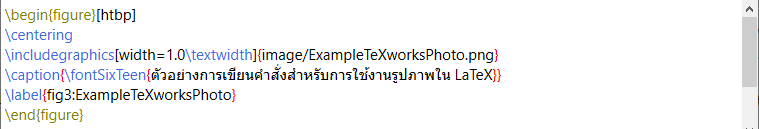
\includegraphics[width=1.0\textwidth]{Image/ExampleTeXworksPhoto.png}
}
\caption{\fontSixTeen{ตัวอย่างการเขียนคำสั่งสำหรับการใช้งานรูปภาพใน LaTeX}}
\label{fig3:ExampleTeXworksPhoto}
\end{figure}

\hspace*{1.5em} %ย่อหน้า
จากภาพที่ \ref{fig3:ExampleTeXworksPhoto} ในการปรับขนาดของรูปภาพให้เหมาะสมกับเอกสาร สามารถใช้ตัวเลือก \textbf{width} ในคำสั่ง \textbf{\textbackslash includegraphics} ซึ่งช่วยให้สามารถกำหนดความกว้างของรูปภาพสัมพันธ์กับความกว้างของหน้ากระดาษได้ ตัวอย่างเช่น \textbf{width=1.0\textbackslash textwidth} หมายถึง การกำหนดให้รูปภาพมีความกว้างเท่ากับความกว้างของเนื้อหาข้อความทั้งหมดบนหน้ากระดาษ (\textbf{\textbackslash textwidth}) ทำให้รูปภาพไม่ล้นขอบหรือเล็กเกินไป ด้วยการปรับค่าตัวเลข (เช่น 0.8) เพื่อปรับความกว้างของรูปภาพตามความเหมาะสม

\subsection{การใช้งานตาราง}
\hspace*{1.5em} %ย่อหน้า
ตาราง (Tables) ถูกใช้เพื่อนำเสนอข้อมูลเชิงตัวเลข คุณสมบัติ หรือข้อมูลเปรียบเทียบในรูปแบบที่เป็นระเบียบ โดยใช้สภาพแวดล้อม \textbf{table} ร่วมกับ \textbf{tabularx} เพื่อให้ตารางสามารถปรับความกว้างของคอลัมน์ได้อัตโนมัติ คำบรรยายตารางจะถูกจัดรูปแบบเป็น \textbf{ฟอนต์หนาขนาด 16pt} ตามที่กำหนดใน \textbf{\textbackslash captionsetup[table]} ของ \textbf{project\_report.cls}


\newpage
\begin{table}[h!]
    \centering
    \caption{\fontSixTeen ตัวอย่างการสร้างตารางด้วย LaTeX}
    \label{tab3:ExampleCreateTable}
    \fontSixTeen 
    \begin{tabularx}{\textwidth}{| c | X | r |} 
    \hline
    \textbf{กึ่งกลาง} 	& \textbf{ชิดซ้าย} 					& \textbf{ชิดขวา} \\
    \hline
    ข้อมูลตรงกลาง      & ข้อมูลนี้จะถูกจัดชิดซ้ายของคอลัมน์			& 1,234.56 		 \\
    หัวข้อ            & รายละเอียดเพิ่มเติม                     & 25 มิถุนายน 2568 \\
    100            	& ข้อความอาจจะยาวกว่านี้เพื่อแสดงการจัดตำแหน่ง & จำนวนรวม 		 \\
    \hline
    \end{tabularx}
\end{table}

\hspace*{1.5em} %ย่อหน้า
จากตารางที่ \ref{tab3:ExampleCreateTable} สร้างจากคำสั่งดังภาพที่ \ref{fig3:ExampleCreateTable} 

\begin{figure}[h!]
\centering
\adjustbox{frame, width=1.0\textwidth}{%สร้างกรอบของภาพ
    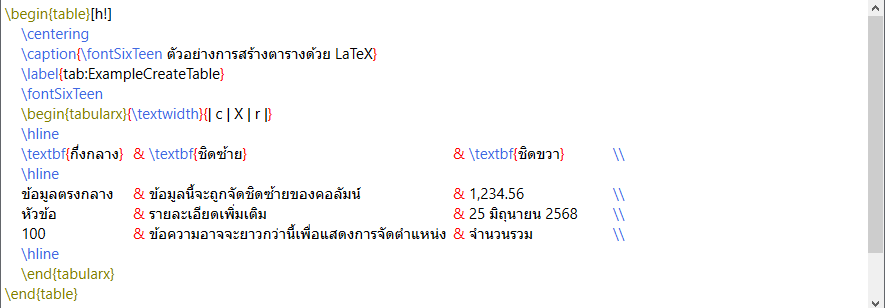
\includegraphics[width=1.0\textwidth]{Image/ExampleCreateTable.png}
}
\caption{\fontSixTeen{ตัวอย่างการเขียนคำสั่งสำหรับการสร้างตาราง}}
\label{fig3:ExampleCreateTable}
\end{figure}

\hspace*{1.5em} %ย่อหน้า
จากคำสั่งดังภาพที่ \ref{fig3:ExampleCreateTable} สามารถอธิบายเพิ่มเติมได้ดังนี้

\begin{mycustomitem}
    \item \textbf{\textbackslash begin\{tabularx\}\{\textbackslash textwidth\}\{...\}} ใช้เมื่อเริ่มต้นสภาพแวดล้อม \textbf{tabularx}
    \begin{mycustomitem}
        \item \textbf{\{\textbackslash textwidth\}} ใช้กำหนดให้ตารางมีความกว้างเต็ม \textbf{ความกว้างของข้อความ} (\textbf{\textbackslash textwidth}) ของหน้ากระดาษ
        \item \textbf{\{| c | X | r |\}} ส่วนนี้คือการ \textbf{กำหนดคุณสมบัติของแต่ละคอลัมน์}
        \begin{mycustomitem}
            \item \textbf{|} คือ การสร้าง \textbf{เส้นแนวตั้ง} คั่นระหว่างคอลัมน์
            \item \textbf{c} คือ คอลัมน์ที่เนื้อหา \textbf{จัดกึ่งกลาง} (centered)
            \item \textbf{X} คือ คอลัมน์พิเศษที่ \textbf{ปรับความกว้างอัตโนมัติ} (variable-width) เพื่อเติมเต็มพื้นที่ว่างที่เหลือ ทำให้ตารางมีความกว้างรวมตามที่กำหนด
            \item \textbf{r} คือ คอลัมน์ที่เนื้อหา \textbf{จัดชิดขวา} (right-aligned)
            \item \textbf{l} (เพิ่มเติม) คอลัมน์ที่เนื้อหา \textbf{จัดชิดซ้าย} (left-aligned)
        \end{mycustomitem}
    \end{mycustomitem}
    \item \textbf{\textbackslash hline} ใช้สำหรับสร้าง \textbf{เส้นแนวนอน} ในตาราง
    \item \textbf{\&} ใช้สำหรับ \textbf{คั่นระหว่างเซลล์} ในแต่ละแถว
    \item \textbf{\textbackslash\textbackslash} ใช้สำหรับ \textbf{ขึ้นบรรทัดใหม่} เพื่อเริ่มแถวใหม่ของตาราง
    \item \textbf{\textbackslash textbf\{\dots\}} ทำให้ข้อความ \textbf{ตัวหนา} เหมาะสำหรับหัวตาราง
\end{mycustomitem}

\newpage
\hspace*{1.5em} %ย่อหน้า
นอกเหนือจาก \textbf{h} ที่ใช้ในตัวอย่าง ยังมีตัวเลือกอื่น ๆ ที่สามารถใส่ใน \textbf{\textbackslash begin\{table\}[...]} เพื่อบอก LaTeX ว่าต้องการให้ตารางไปปรากฏที่ใด

\begin{mycustomitem}
    \item \textbf{h} (here) พยายามวางตาราง \textbf{ตรงตำแหน่งที่โค้ดปรากฏ} ในไฟล์
    \item \textbf{t} (top) พยายามวางตารางที่ \textbf{ด้านบนสุดของหน้า} ปัจจุบันหรือหน้าถัดไป
    \item \textbf{b} (bottom) พยายามวางตารางที่ \textbf{ด้านล่างสุดของหน้า} ปัจจุบันหรือหน้าถัดไป
    \item \textbf{p} (page) นำตารางไปรวมไว้ใน \textbf{หน้าเฉพาะที่รวบรวมตาราง/รูปภาพ} เท่านั้น
    \item \textbf{!} (override) ใช้ \textbf{ร่วมกับ} ตัวเลือกอื่นๆ (เช่น \textbf{[h!]}, \textbf{[t!]}) เพื่อ \textbf{บังคับ} ให้ LaTeX พยายามวางตามตำแหน่งที่ระบุให้ได้ แม้จะต้องละเมิดกฎการจัดวางบางอย่าง
\end{mycustomitem}

\hspace*{1.5em} %ย่อหน้า
นอกจากนี้ยังสามารถรวมตัวเลือกเหล่านี้ได้ เช่น \textbf{[htb!]} เพื่อให้ LaTeX พยายามวางจาก "here" ก่อน ถ้าไม่ได้ก็ "top" ถ้าไม่ได้ก็ "bottom" และใช้ \textbf{!} เพื่อบังคับ


\subsection{การสร้างรายการ (Lists)}
\hspace*{1.5em} %ย่อหน้า
สำหรับรายการแบบลำดับ ผู้จัดทำได้ใช้สภาพแวดล้อมที่กำหนดเองในไฟล์คลาส ได้แก่ \textbf{mycustomenum}, \textbf{mycustomenum2} (สำหรับรายการลำดับเลข) และ \textbf{mycustomitem} (สำหรับรายการด้วยเครื่องหมาย) ซึ่งมีการกำหนดระยะเยื้องและรูปแบบของตัวเลข/สัญลักษณ์นำหน้าด้วยเครื่องหมายขีด

\hspace*{1.5em} %ย่อหน้า
\textbf{ตัวอย่างการใช้ \textbf{mycustomenum}} 
\begin{mycustomenum}[label=1.1.\arabic*]
    \item รายการระดับที่ 1 รายการระดับที่ 1 รายการระดับที่ 1 รายการระดับที่ 1  รายการระดับที่ 1 รายการระดับที่ 1
    \item รายการระดับที่ 1
    \begin{mycustomenum}
        \item รายการระดับที่ 2
        \begin{mycustomenum}
            \item รายการระดับที่ 3
            \item รายการระดับที่ 3 รายการระดับที่ 3 รายการระดับที่ 3 รายการระดับที่ 3 
        \end{mycustomenum}
        \item รายการระดับที่ 2 รายการระดับที่ 2 รายการระดับที่ 2 รายการระดับที่ 2
    \end{mycustomenum}
    \item รายการระดับที่ 1
    \item รายการระดับที่ 1
\end{mycustomenum}

\newpage
\hspace*{1.5em} %ย่อหน้า
จากตัวอย่างการใช้งาน mycustomenum ข้างต้น ตัวอย่างคำสั่งแสดงได้ดังภาพที่ \ref{fig3:ExampleCreateEnum} 

\begin{figure}[htbp]
\centering
\adjustbox{frame, width=1.0\textwidth}{%สร้างกรอบของภาพ
    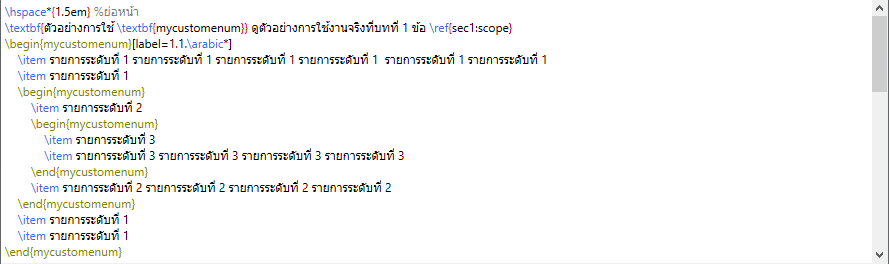
\includegraphics[width=1.0\textwidth]{Image/ExampleCreateEnum.png}
}
\caption{\fontSixTeen{ตัวอย่างการเขียนคำสั่งสำหรับการสร้างรายการด้วยคลาส mycustomenum}}
\label{fig3:ExampleCreateEnum}
\end{figure}



\hspace*{1.5em} %ย่อหน้า
\textbf{ตัวอย่างการใช้ \textbf{mycustomenum2}}
\begin{mycustomenum2}
    \item รายการระดับที่ 1
    \item รายการระดับที่ 1
    \begin{mycustomenum2}
        \item รายการระดับที่ 2
        \begin{mycustomenum2}
            \item รายการระดับที่ 3 รายการระดับที่ 3 รายการระดับที่ 3 รายการระดับที่ 3 รายการระดับที่ 3 รายการระดับที่ 3 รายการระดับที่ 3 
            \item รายการระดับที่ 3
        \end{mycustomenum2}
        \item รายการระดับที่ 2
        \item รายการระดับที่ 2
    \end{mycustomenum2}
\end{mycustomenum2}

\hspace*{1.5em} %ย่อหน้า
จากตัวอย่างการใช้งาน mycustomenum2 ข้างต้น ตัวอย่างคำสั่งแสดงได้ดังภาพที่ \ref{fig3:ExampleCreateEnum2} 

\begin{figure}[htbp]
\centering
\adjustbox{frame, width=1.0\textwidth}{%สร้างกรอบของภาพ
    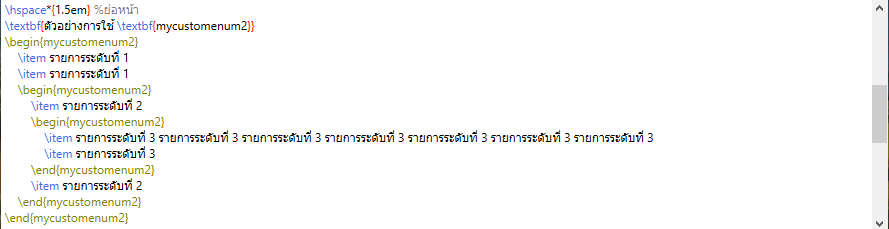
\includegraphics[width=1.0\textwidth]{Image/ExampleCreateEnum2.png}
}
\caption{\fontSixTeen{ตัวอย่างการเขียนคำสั่งสำหรับการสร้างรายการด้วยคลาส mycustomenum2}}
\label{fig3:ExampleCreateEnum2}
\end{figure}


\hspace*{1.5em} %ย่อหน้า
\textbf{ตัวอย่างการใช้ \textbf{mycustomitem}}
\begin{mycustomitem}
    \item รายการระดับที่ 1
    \item รายการระดับที่ 1
    \begin{mycustomitem}
        \item รายการระดับที่ 2
        \begin{mycustomitem}
            \item รายการระดับที่ 3 รายการระดับที่ 3 รายการระดับที่ 3 รายการระดับที่ 3 รายการระดับที่ 3 รายการระดับที่ 3 รายการระดับที่ 3 
            \item รายการระดับที่ 3
        \end{mycustomitem}
        \item รายการระดับที่ 2
    \end{mycustomitem}
\end{mycustomitem}


\hspace*{1.5em} %ย่อหน้า
จากตัวอย่างการใช้งาน mycustomitem ข้างต้น ตัวอย่างคำสั่งแสดงได้ดังภาพที่ \ref{fig3:ExampleCreateItem} 

\begin{figure}[htbp]
\centering
\adjustbox{frame, width=1.0\textwidth}{%สร้างกรอบของภาพ
    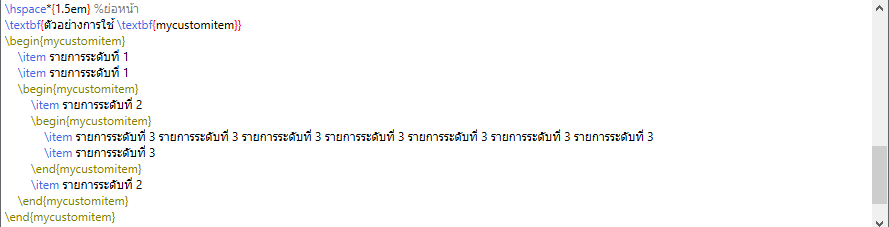
\includegraphics[width=1.0\textwidth]{Image/ExampleCreateItem.png}
}
\caption{\fontSixTeen{ตัวอย่างการเขียนคำสั่งสำหรับการสร้างรายการด้วยคลาส mycustomitem}}
\label{fig3:ExampleCreateItem}
\end{figure}


\hspace*{1.5em} %ย่อหน้า
\textbf{ตัวอย่างการใช้งาน mycustomenum2 และ mycustomitem ร่วมกัน}
\begin{mycustomenum2}
    \item รายการระดับที่ 1
    \item รายการระดับที่ 1
    \begin{mycustomenum2}
        \item รายการระดับที่ 2
        \begin{mycustomitem}[leftmargin=0.7cm,labelwidth=0.7cm]
            \item รายการระดับที่ 3
            \item รายการระดับที่ 3
        \end{mycustomitem}
        \item รายการระดับที่ 2
        \begin{mycustomitem}[leftmargin=0.7cm,labelwidth=0.7cm]
            \item รายการระดับที่ 3
            \begin{mycustomitem}
                \item รายการระดับที่ 4
                \item รายการระดับที่ 4
            \end{mycustomitem}
            \item รายการระดับที่ 3
        \end{mycustomitem}
        \item รายการระดับที่ 2
        \item รายการระดับที่ 2
    \end{mycustomenum2}
    \item รายการระดับที่ 1
    \begin{mycustomenum2}
        \item รายการระดับที่ 2
        \begin{mycustomenum2}
            \item รายการระดับที่ 3
            \begin{mycustomitem}[leftmargin=0.7cm,labelwidth=0.7cm]
                \item รายการระดับที่ 4
                \item รายการระดับที่ 4
            \end{mycustomitem}
            \item รายการระดับที่ 3
            \item รายการระดับที่ 3
        \end{mycustomenum2}
        \item รายการระดับที่ 2
    \end{mycustomenum2}
    \item รายการระดับที่ 1
    \item รายการระดับที่ 1
\end{mycustomenum2}


\hspace*{1.5em} %ย่อหน้า
จากตัวอย่างการใช้งาน mycustomenum2 และ mycustomitem ร่วมกันข้างต้น ตัวอย่างคำสั่งแสดงได้ดังภาพที่ \ref{fig3:ExampleCreateEnum2MixItem}

\begin{figure}[htbp]
\centering
\adjustbox{frame, width=1.0\textwidth}{%สร้างกรอบของภาพ
    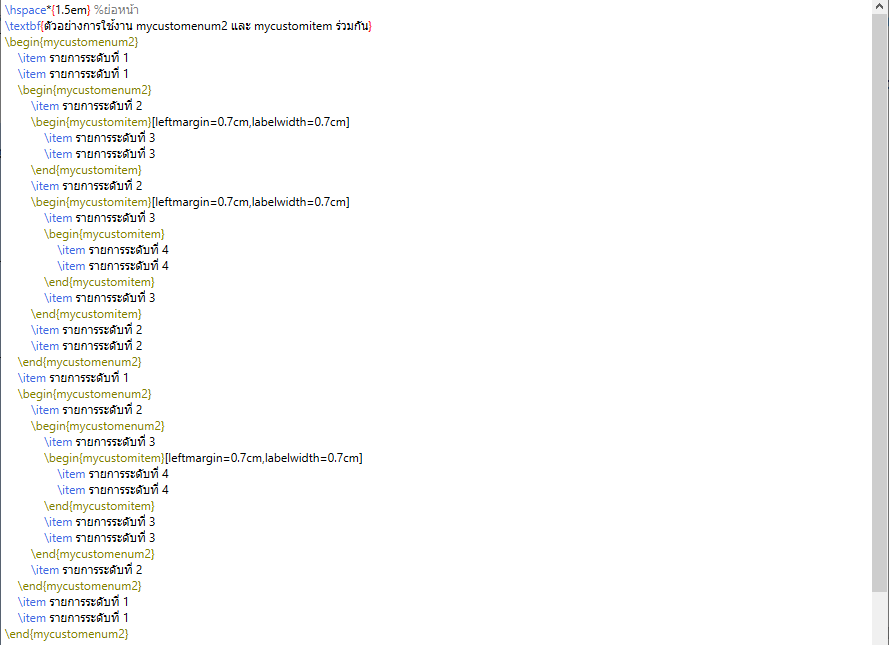
\includegraphics[width=1.0\textwidth]{Image/ExampleCreateEnum2MixItem.png}
}
\caption{\fontSixTeen{ตัวอย่างการเขียนคำสั่งสำหรับการสร้างรายการด้วยคลาส mycustomenum2 และ mycustomitem ร่วมกัน}}
\label{fig3:ExampleCreateEnum2MixItem}
\end{figure}



\subsection{การจัดการบรรณานุกรม}
\hspace*{1.5em} %ย่อหน้า
ในส่วนของการจัดการบรรณานุกรม มีรายละเอียดดังนี้

\begin{mycustomitem}
    \item ไฟล์ \textbf{.bib} (เช่น \textbf{Project\_999\_Bibliography.bib}) ได้ถูกสร้างไว้แล้วสำหรับรวบรวมข้อมูลบรรณานุกรมทั้งหมด
    \item ใช้คำสั่ง \textbf{\textbackslash addbibresource\{Project\_999\_Bibliography.bib\}} ใน Preamble ของเอกสาร และ \textbf{\textbackslash printbibliography} ในส่วนท้ายของเอกสารเพื่อสร้างหน้าบรรณานุกรม
    \item มีการกำหนดหัวเรื่องบรรณานุกรมด้วย \textbf{\textbackslash defbibheading\{mybibheading\}} ให้แสดง \textbf{บรรณานุกรม} และ \textbf{บรรณานุกรม (ต่อ)} พร้อมเลขหน้าตามที่กำหนดไว้ในไฟล์คลาส
\end{mycustomitem}


\hspace*{1.5em} %ย่อหน้า
ตัวอย่างการเขียนบรรณานุกรมในไฟล์ .bib แสดงได้ดังภาพที่ \ref{fig3:ExampleBib}

\begin{figure}[htbp]
\centering
\adjustbox{frame, width=1.0\textwidth}{%สร้างกรอบของภาพ
    
\includegraphics[width=1.0\textwidth]{Image/ExampleBib.png}
}
\caption{\fontSixTeen{ตัวอย่างการเขียนข้อมูลบรรณานุกรมใน bib file}}
\label{fig3:ExampleBib}
\end{figure}

\hspace*{1.5em} %ย่อหน้า
ตัวอย่างการเขียนอ้างอิงในเนื้อหา ด้วยคำสั่ง \textbf{\textbackslash parencite\{Tanya2008\}} แสดงได้ดังภาพที่ \ref{fig3:ExampleRefInContent}

\begin{figure}[htbp]
\centering
\adjustbox{frame, width=1.0\textwidth}{%สร้างกรอบของภาพ
    
\includegraphics[width=1.0\textwidth]{Image/ExampleRefInContent.png}
}
\caption{\fontSixTeen{ตัวอย่างการเขียนอ้างอิงในเนื้อหา}}
\label{fig3:ExampleRefInContent}
\end{figure}


    %*************************************
% บทที่ 4
%*************************************
\chapterTitle{4}{ผลการดำเนินงาน}

\hspace*{1.5em}
ในการพัฒนา Template สำหรับการจัดทำเล่มปริญญานิพนธ์ด้วย LaTeX จัดทำขึ้นเพื่ออำนวยความสะดวกให้แก่นักศึกษาในภาควิชาเทคโนโลยีสารสนเทศ ให้สามารถจัดรูปเล่มได้ถูกต้องตามรูปแบบมาตรฐานที่กำหนด ในส่วนของผลการดำเนินงานที่ได้ประกอบด้วยไฟล์โครงสร้างและการปรับแต่งรูปแบบเอกสาร
ตั้งแต่หน้าปก ปกในภาษาไทย ปกในภาษาอังกฤษ ใบรับรองปริญญานิพนธ์ บทคัดย่อภาษาไทย บทคัดย่อภาษาอังกฤษ กิตติกรรมประกาศ สารบัญ สารบัญภาพ สารบัญตาราง บทเนื้อหา บรรณานุกรม และภาคผนวก
ทั้งนี้ ผู้จัดทำได้ทดสอบการใช้งาน Template ดังกล่าว โดยตรวจสอบการจัดหน้า การอ้างอิง และรูปแบบการนำเสนอ เพื่อให้มั่นใจว่าสามารถนำไปใช้งานได้จริง สอดคล้องตามคู่มือการจัดทำเล่มวิทยานิพนธ์ของภาควิชา
\section{โครงสร้างโฟลเดอร์}
\hspace*{1.5em}
จากการออกแบบและพัฒนา Template ของรูปเล่มปริญญานิพนธ์ด้วย LaTeX ประกอบไปด้วย 3 โฟลเดอร์หลัก ได้แก่ 

\subsection{โฟลเดอร์ Class}
\hspace*{1.5em}
โฟลเดอร์ \textbf{Class} เป็นที่เก็บไฟล์รูปแบบเอกสารหลัก \textbf{project\_report.cls} เป็นไฟล์คลาส (Class File) ที่เขียนด้วยภาษา LaTeX มีหน้าที่กำหนดรูปแบบของการจัดรูปเล่มปริญญานิพนธ์ เช่น ขนาดกระดาษ และระยะขอบหน้า-หลัง รูปแบบและขนาดตัวอักษร รูปแบบบทและหัวข้อย่อย รวมทั้งการจัดวางสารบัญ ตาราง รูปภาพ และบรรณานุกรม

\subsection{โฟลเดอร์ Font}
\hspace*{1.5em}
โฟลเดอร์ \textbf{Font} ใช้สำหรับเก็บไฟล์ฟอนต์ที่จำเป็นต้องใช้ในการจัดรูปแบบรูปเล่มปริญญานิพนธ์ ภายในโฟลเดอร์นี้จะเก็บไฟล์ฟอนต์ \textbf{TH Sarabun New} ซึ่งเป็นฟอนต์ภาษาไทยมาตรฐาน 
ที่มีรูปแบบตัวอักษรชัดเจนและเหมาะสมสำหรับงานวิชาการ ตัวอย่างไฟล์ฟอนต์ที่เก็บ ได้แก่
\begin{mycustomenum2}
  \item \textbf{THSarabunNew.ttf}
  \item \textbf{THSarabunNew Bold.ttf}
  \item \textbf{THSarabunNew Italic.ttf}
  \item \textbf{THSarabunNew BoldItalic.ttf}
\end{mycustomenum2}
\hspace*{1.5em}
การเก็บฟอนต์ในโฟลเดอร์ \textbf{Font} จะช่วยให้โครงสร้างโปรเจกต์เป็นระเบียบ 
และสะดวกต่อการจัดการไฟล์ฟอนต์เมื่อย้ายไปใช้งานในเครื่องคอมพิวเตอร์อื่น ๆ 

\subsection{โฟลเดอร์ Image}
\hspace*{1.5em}
โฟลเดอร์ \textbf{Image} ใช้สำหรับเก็บไฟล์รูปภาพประกอบที่ใช้ในรูปเล่มปริญญานิพนธ์ โดยการแยกรูปภาพไว้ในโฟลเดอร์นี้จะช่วยให้การจัดการไฟล์ง่ายขึ้นและป้องกันความสับสนกับไฟล์อื่น ๆ เช่น ไฟล์โค้ดหรือไฟล์เอกสารหลัก โดยทั่วไปแล้วไฟล์รูปภาพที่ใช้ใน LaTeX ควรอยู่ในรูปแบบที่เหมาะสม เช่น PNG หรือ JPG เพื่อให้สามารถแสดงผลได้ถูกต้องและมีคุณภาพสูง

\section{โครงสร้างไฟล์}
\subsection{ไฟล์เอกสารหลัก}
\hspace*{1.5em}
นอกจากโฟลเดอร์ทั้งสามที่กล่าวมาแล้ว ในโครงสร้างโปรเจกต์ยังมีไฟล์เอกสารหลักที่สำคัญอีกหนึ่งไฟล์ คือ \textbf{Main.tex} ซึ่งเป็นไฟล์หลักที่ใช้ในการรวบรวมเนื้อหาทั้งหมดของปริญญานิพนธ์เข้าไว้ด้วยกัน ไฟล์นี้จะทำหน้าที่เรียกใช้ไฟล์คลาส (\textbf{project\_report.cls}) เพื่อกำหนดรูปแบบหน้ากระดาษ รวมถึงเรียกใช้เนื้อหาในแต่ละบท (เช่น บทนำ ทฤษฎีที่เกี่ยวข้อง วิธีการดำเนินงาน ผลการทดลอง) และองค์ประกอบอื่น ๆ เช่น สารบัญ สารบัญตาราง สารบัญรูปภาพ และบรรณานุกรม ทำให้ผู้ใช้งานสามารถจัดการเนื้อหาแต่ละส่วนได้อย่างเป็นระบบและง่ายต่อการแก้ไข

\subsection{ตัวอย่างโครงสร้างไฟล์ทั้งหมด}
\hspace*{1.5em}
ภาพที่ \ref{fig4:StructureFile} แสดงตัวอย่างโครงสร้างไฟล์ทั้งหมดที่ใช้ในการจัดทำรูปเล่มปริญญานิพนธ์ด้วย LaTeX จะเห็นว่ามีการจัดระเบียบไฟล์อย่างเป็นระบบ เพื่อความสะดวกในการจัดการและแก้ไขเนื้อหา โดยโครงสร้างประกอบด้วยโฟลเดอร์หลัก 3 โฟลเดอร์ ได้แก่ Class, Font และ Image ซึ่งทำหน้าที่เก็บไฟล์ที่เกี่ยวข้องกับการตั้งค่า รูปแบบตัวอักษร และรูปภาพตามลำดับ อีกทั้งยังมีไฟล์หลัก \textbf{Main.tex} และไฟล์คลาส (\textbf{project\_report.cls}) ดังที่กล่าวไว้ข้างต้น

\hspace*{1.5em}
นอกจากนี้ยังประกอบด้วยไฟล์หลักอีกหลายไฟล์ ได้แก่
\begin{mycustomitem}
    \item Project\_000\_Cover.tex สำหรับปก
    \item Project\_001\_Certificate.tex สำหรับใบรับรองปริญญานิพนธ์ ซึ่งจะมีด้วยกัน 2 ไฟล์ให้เลือกใช้ 
    \begin{mycustomitem}
        \item Project\_001\_Certificate1.tex ในกรณีไม่มีที่ปรึกษาร่วม และ 
        \item Project\_001\_Certificate2.tex กรณีมีที่ปรึกษาร่วม 
    \end{mycustomitem}
    (กำหนดที่ไฟล์ Main.tex)
    \item Project\_002\_Abstract.tex สำหรับบทคัดย่อ
    \item Project\_010\_Chapter1.tex สำหรับบทที่ 1 และ 
    \item Project\_999\_Bibliography.bib สำหรับบรรณานุกรม
\end{mycustomitem}
\hspace*{1.5em}
การแบ่งไฟล์เป็นส่วนย่อยเช่นนี้ช่วยให้การจัดการเนื้อหาแต่ละส่วนมีความเป็นระเบียบ และง่ายต่อการทำงานร่วมกันเป็นทีม เมื่อต้องการแก้ไขเนื้อหาในบทใดบทหนึ่งก็สามารถเข้าไปแก้ไขได้โดยตรงในไฟล์นั้น ๆ โดยไม่กระทบกับส่วนอื่น ๆ ของรูปเล่ม 

\begin{figure}[htbp]
\centering
\adjustbox{frame, width=0.6\textwidth}{
    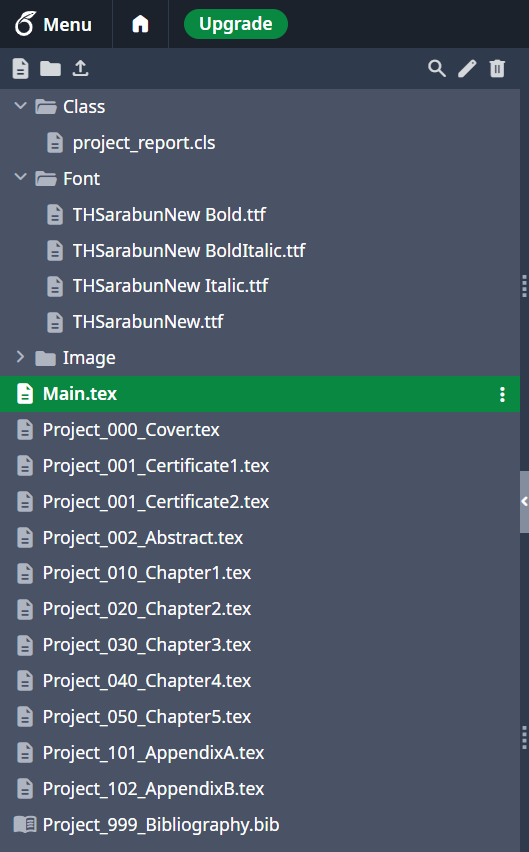
\includegraphics[width=0.6\textwidth]{Image/Structure_files.png}
}
\caption{\fontSixTeen{โครงสร้างไฟล์ทั้งหมด}}
\label{fig4:StructureFile}
\end{figure}

\hspace*{1.5em}
การจัดโครงสร้างไฟล์ในลักษณะนี้ไม่เพียงแต่ช่วยให้โปรเจกต์เป็นระเบียบ แต่ยังช่วยลดความซับซ้อนในการจัดการไฟล์จำนวนมาก ทำให้การทำงานเป็นทีมง่ายขึ้น และสามารถนำไปใช้งานต่อหรือแก้ไขในอนาคตได้อย่างสะดวกและมีประสิทธิภาพ
    %*************************************
% บทที่ 5
%*************************************
\chapterTitle{5}{สรุปผลการดำเนินงาน}

\section{สรุปผลการดำเนินงาน}
\hspace*{1.5em}
โครงการ "การจัดทำรูปเล่มปริญญานิพนธ์ด้วย LaTeX" ได้พัฒนาแม่แบบ (Template) สำหรับการเขียนรูปเล่มปริญญานิพนธ์โดยใช้ LaTeX โดยมีการรวบรวมคำสั่งพื้นฐานที่จำเป็นและปรับโครงสร้างเอกสารให้สอดคล้องกับมาตรฐานของภาควิชาเทคโนโลยีสารสนเทศ ผลลัพธ์ที่สำคัญของโครงการคือการสร้างแม่แบบ LaTeX ที่สมบูรณ์ ซึ่งครอบคลุมทุกส่วนของรูปเล่มปริญญานิพนธ์ ตั้งแต่หน้าปก สารบัญ สารบัญรูปภาพ สารบัญตาราง เนื้อหา ภาคผนวก และบรรณานุกรม ทำให้ผู้ใช้สามารถนำไปใช้งานได้ทันทีและช่วยลดเวลาในการจัดรูปแบบเอกสารได้อย่างมาก ส่งผลให้ผู้จัดทำมุ่งเน้นไปที่การเขียนเนื้อหาทางวิชาการได้อย่างเต็มที่

\section{ปัญหาและอุปสรรค}
\begin{mycustomenum}[label=5.2.\arabic*] 
    \item ความซับซ้อนของ LaTeX เนื่องจาก LaTeX มีคำสั่งและโครงสร้างที่ต้องเรียนรู้มากมาย ทำให้ผู้เริ่มต้นใช้งานต้องใช้เวลาในการทำความเข้าใจ
    \item การจัดบรรณานุกรม (Bibliography) ไฟล์ .bib ถูกใช้เพื่อจัดการข้อมูลบรรณานุกรม อาจมีความซับซ้อนสำหรับผู้ใช้ที่ยังไม่คุ้นเคย
    \item การจัดการรูปภาพและตาราง ในการปรับขนาดและตำแหน่งของรูปภาพหรือตารางให้เหมาะสมในเอกสารเป็นเรื่องที่ต้องอาศัยการลองผิดลองถูกพอสมควร
    \item การแก้ไขข้อผิดพลาด (Errors) เมื่อเกิดข้อผิดพลาดในเอกสาร LaTeX การทำความเข้าใจและแก้ไขข้อผิดพลาดเหล่านั้นอาจเป็นเรื่องที่ท้าทาย
\end{mycustomenum}

\section{การแก้ปัญหา}
\begin{mycustomenum}[label=5.3.\arabic*] 
    \item จัดทำตัวอย่างของการนำ LaTex มาใช้งานพร้อมตัวอย่างโค้ดที่ง่ายต่อการทำความเข้าใจ พร้อมภาพประกอบและคำอธิบายทีละขั้นตอน
    \item เลือกใช้แพ็กเกจที่เหมาะสม เลือกใช้แพ็กเกจ LaTeX ที่ใช้งานง่ายและเป็นที่นิยม 
    \item สร้างโค้ดตัวอย่างสำหรับรูปแบบการจัดวางรูปภาพและตารางที่ใช้บ่อย เช่น โค้ดสำหรับรูปภาพขนาดเต็มหน้า โค้ดสำหรับตารางที่มีขนาดพอดีกับหน้ากระดาษ เพื่อให้ผู้ใช้สามารถคัดลอกและนำไปปรับใช้ได้ทันที
\end{mycustomenum}

\section{ข้อเสนอแนะ}
\begin{mycustomenum}[label=5.4.\arabic*] 
    \item พัฒนาฟังก์ชันการใช้งานเพิ่มเติม เช่น การสร้างดัชนี (Index) หรือการเพิ่มความสามารถในการปรับแต่งรูปแบบต่างๆ ให้หลากหลายมากขึ้น
    \item จัดอบรมเชิงปฏิบัติการเพื่อสอนการใช้งาน LaTeX เพื่อให้สามารถใช้งานโปรแกรมได้อย่างมีประสิทธิภาพมากขึ้น 
\end{mycustomenum}

    \newgeometry{a4paper,top=1in,bottom=1in,left=1.5in,right=1in,includehead}
    \setTHSarabunFont
    \fontsize{16}{16}\selectfont
    \arabicPageTopRight
    \printbibliography[heading=mybibheading]
    \clearpage % ขึ้นหน้าใหม่หลังจากหน้าที่มีการปรับ margin
    \restoregeometry % คืนค่า geometry กลับเป็นค่าเริ่มต้น
    \fancyhf{} % ล้างการตั้งค่า fancyhdr ของหน้าที่ปรับ
    \setlength{\headsep}{0in}
    
    \appendixTitlePage
    %*************************************
% ภาคผนวก ก.
%*************************************
\appendixChapterTitle{ก}{การนำ Template มาใช้งาน}
\section{การนำ Template มาใช้งาน}
\hspace*{1.5em}
ในการนำ Template มาใช้งาน วิธีการหนึ่งที่สามารถทำได้ง่าย คือใช้งานผ่านเว็บไซต์ Overleaf โดยเริ่มต้นตั้งแต่การสมัครสมาชิก Overleaf และวิธีการอัปโหลด Template เข้าสู่ระบบ พร้อมอธิบายส่วนประกอบต่างๆ ของหน้าจอการใช้งาน เพื่อให้ผู้ใช้สามารถแก้ไขและปรับแต่งเนื้อหาในรูปเล่มปริญญานิพนธ์ได้ทันที รายละเอียดการนำ Template มาใช้งานด้วยเว็บไซด์ Overleaf มีดังนี้ 

\vspace{0.5em}
\textbf{การสมัครสมาชิก Overleaf}
\vspace{0.5em}

\begin{mycustomenum2}
    \item ไปที่เว็บไซต์ Overleaf (\href{http://www.overleaf.com}{www.overleaf.com}) ตัวอย่างหน้าเว็บไซต์ Overleaf แสดงได้ดังภาพที่ \ref{figA:WebSiteOverleaf1}

\begin{figure}[htbp]
\centering
\adjustbox{frame, width=0.8\textwidth}{
    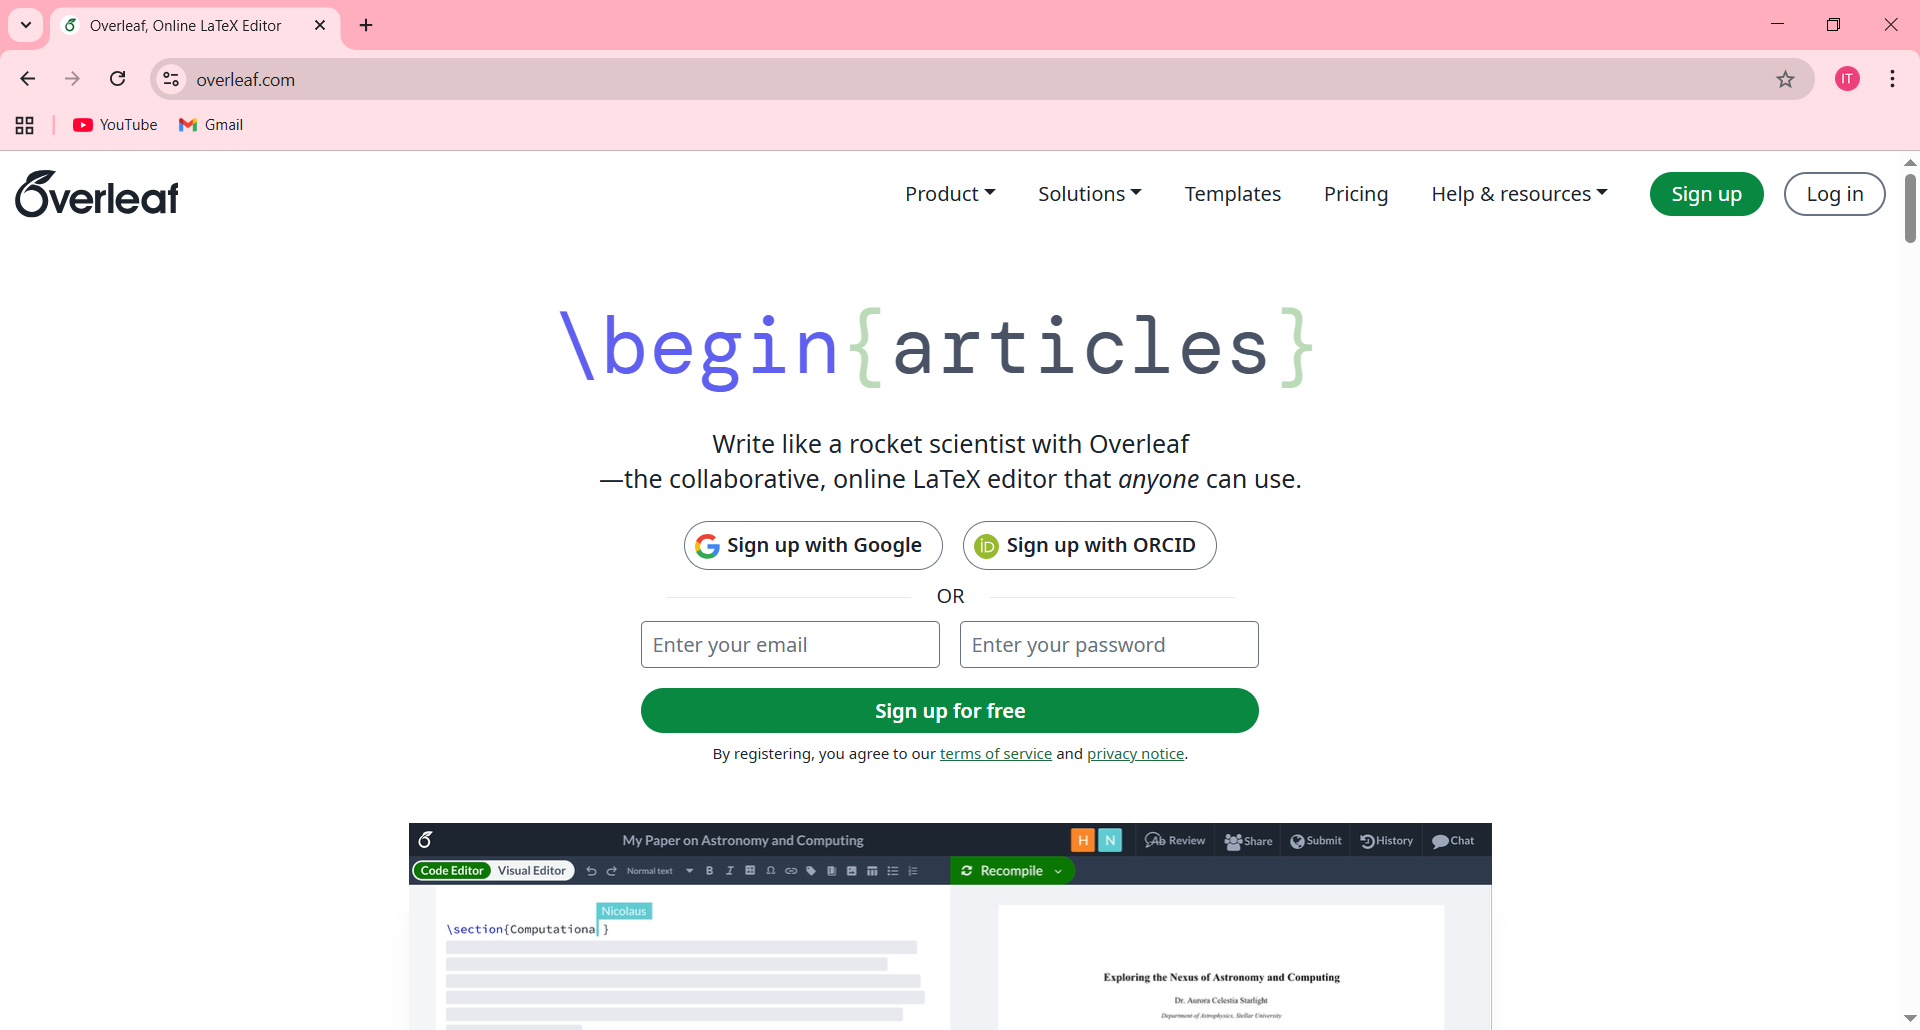
\includegraphics[width=0.8\textwidth]{Image/Overfeaf-1.png}
}
\caption{\fontSixTeen{หน้าแรกของเว็บไซต์ Overleaf}}
\label{figA:WebSiteOverleaf1}
\end{figure}

    \item ที่หน้าแรกดังภาพที่ \ref{figA:WebSiteOverleaf1} ในกรณีที่ยังไม่ได้เป็นสมาชิกให้คลิกที่ \enquote{Sign up} ก็จะพบกับหน้าจอดังภาพที่ \ref{figA:WebSiteOverleaf2}

\begin{figure}[htbp]
\centering
\adjustbox{frame, width=0.8\textwidth}{
    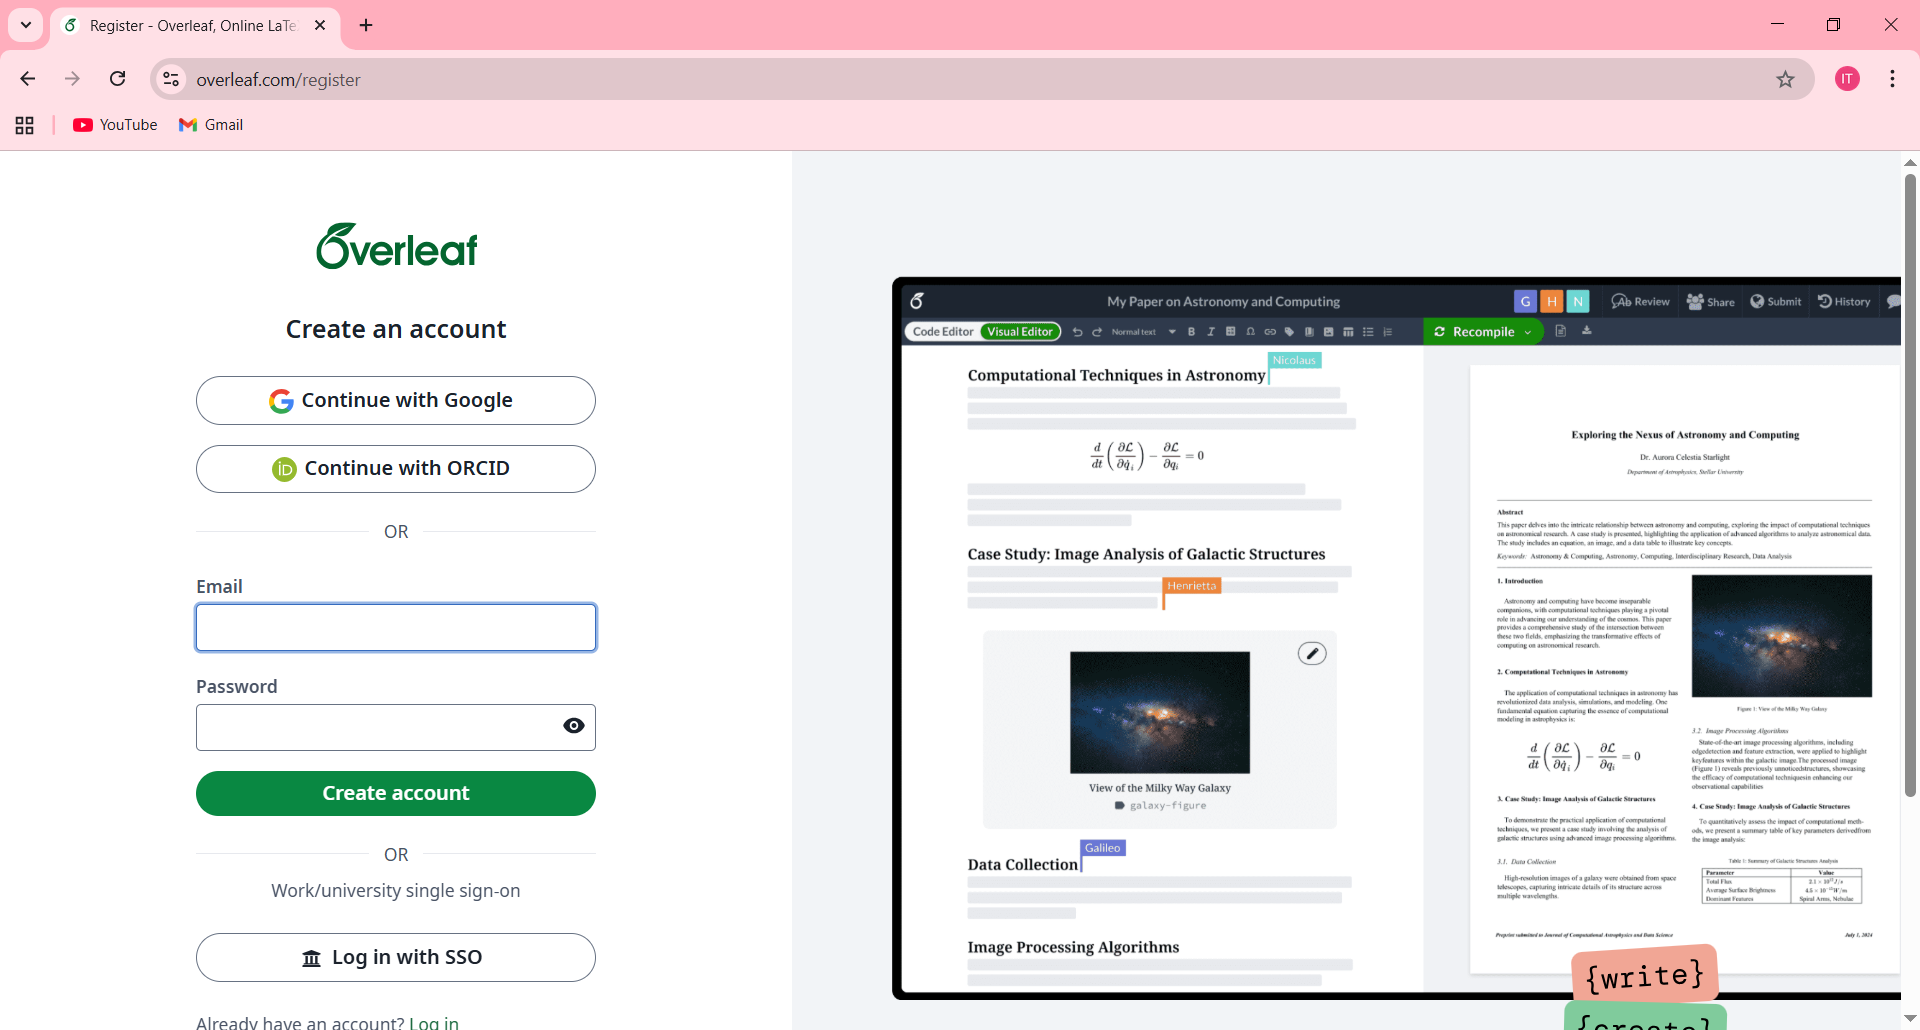
\includegraphics[width=0.8\textwidth]{Image/Overfeaf-2.png}
}
\caption{\fontSixTeen{หน้า Sign up ของเว็บไซต์ Overleaf}}
\label{figA:WebSiteOverleaf2}
\end{figure}

    \item ผู้ใช้งานสามารถเลือกสมัครสมาชิกได้หลายวิธี เช่น
    \begin{mycustomenum2}
        \item สมัครด้วยอีเมล โดยกรอกชื่อ อีเมล และรหัสผ่านที่ต้องการ
        \item สมัครด้วย Google mail ซึ่งเป็นวิธีที่ง่ายและรวดเร็ว 
        \begin{mycustomenum2}
            \item หลังจากคลิกที่ \enquote{Continue with Google} แสดงได้ดังภาพที่ \ref{figA:WebSiteOverleaf3}

\begin{figure}[htbp]
\centering
\adjustbox{frame, width=0.8\textwidth}{
    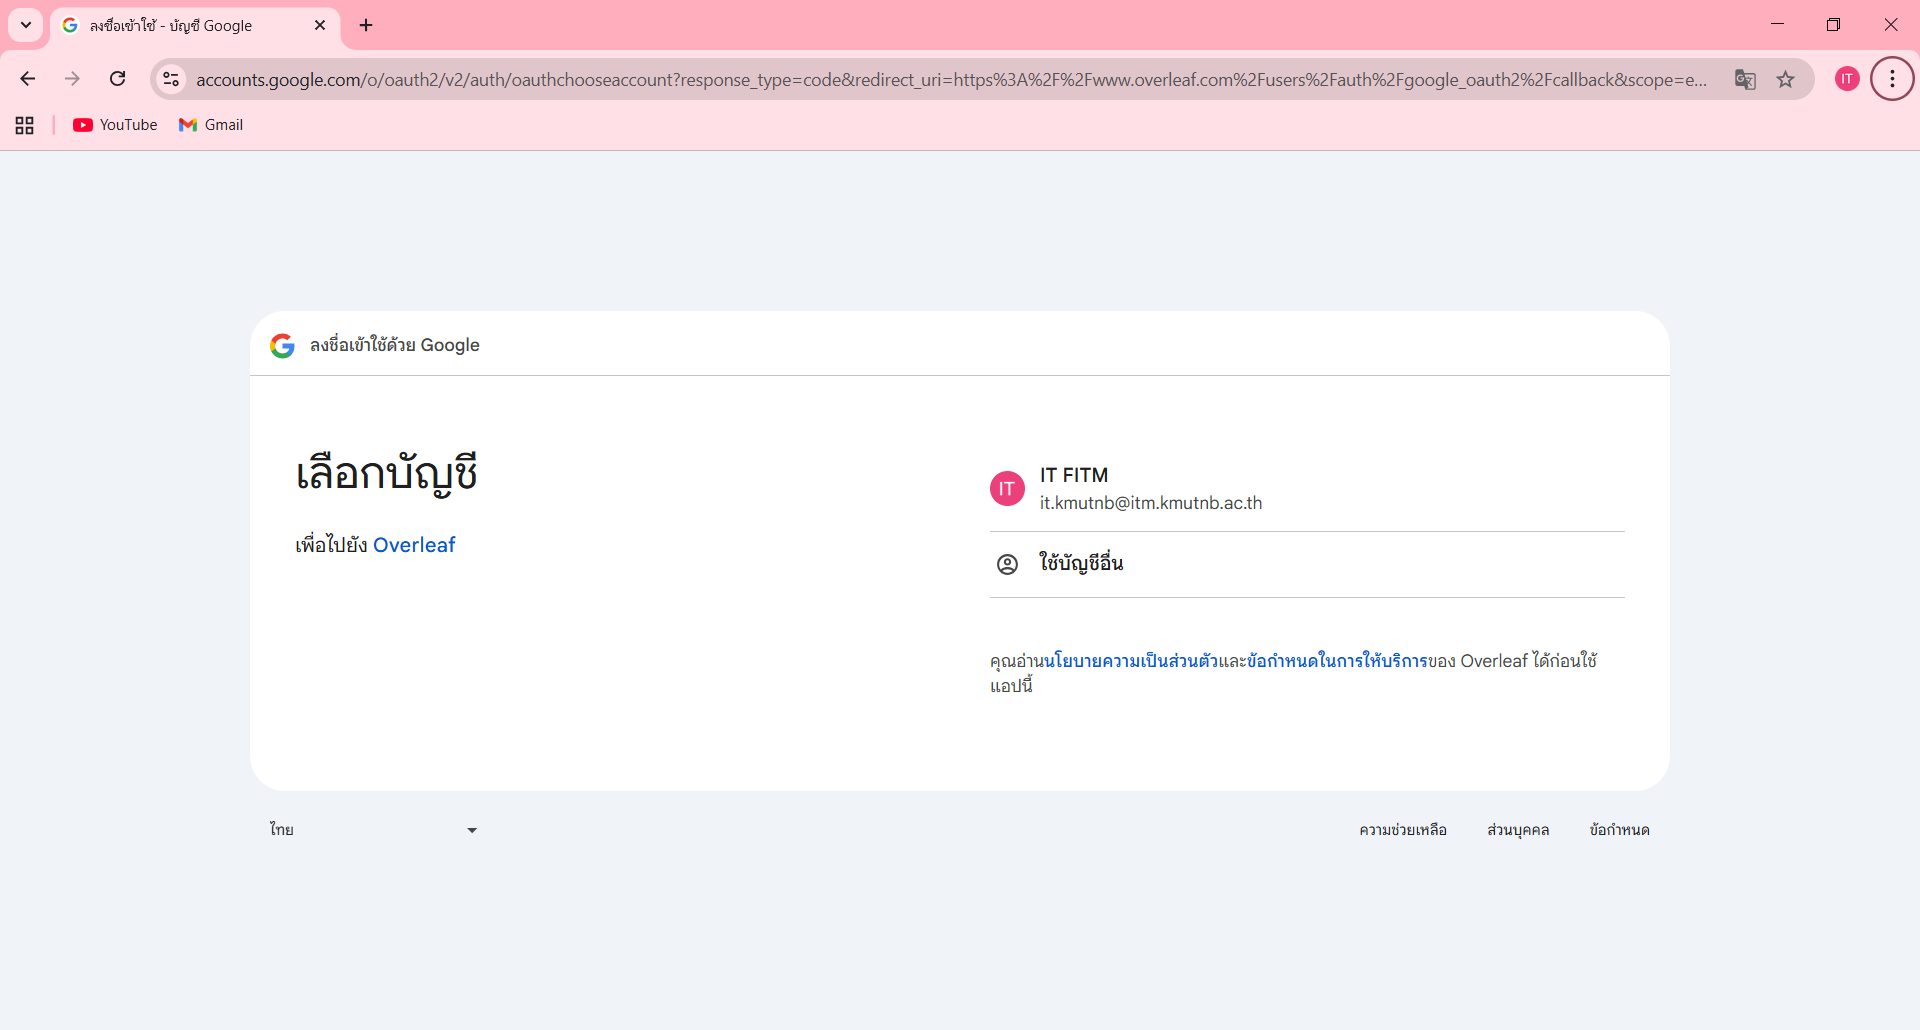
\includegraphics[width=0.8\textwidth]{Image/Overfeaf-3.png}
}
\caption{\fontSixTeen{หน้าเลือกบัญชี Google สำหรับสมัครสมาชิก}}
\label{figA:WebSiteOverleaf3}
\end{figure}

            \item คลิกเลือกบัญชีที่ต้องการเชื่อมต่อ แสดงดังภาพที่ \ref{figA:WebSiteOverleaf4}

\begin{figure}[htbp]
\centering
\adjustbox{frame, width=0.8\textwidth}{
    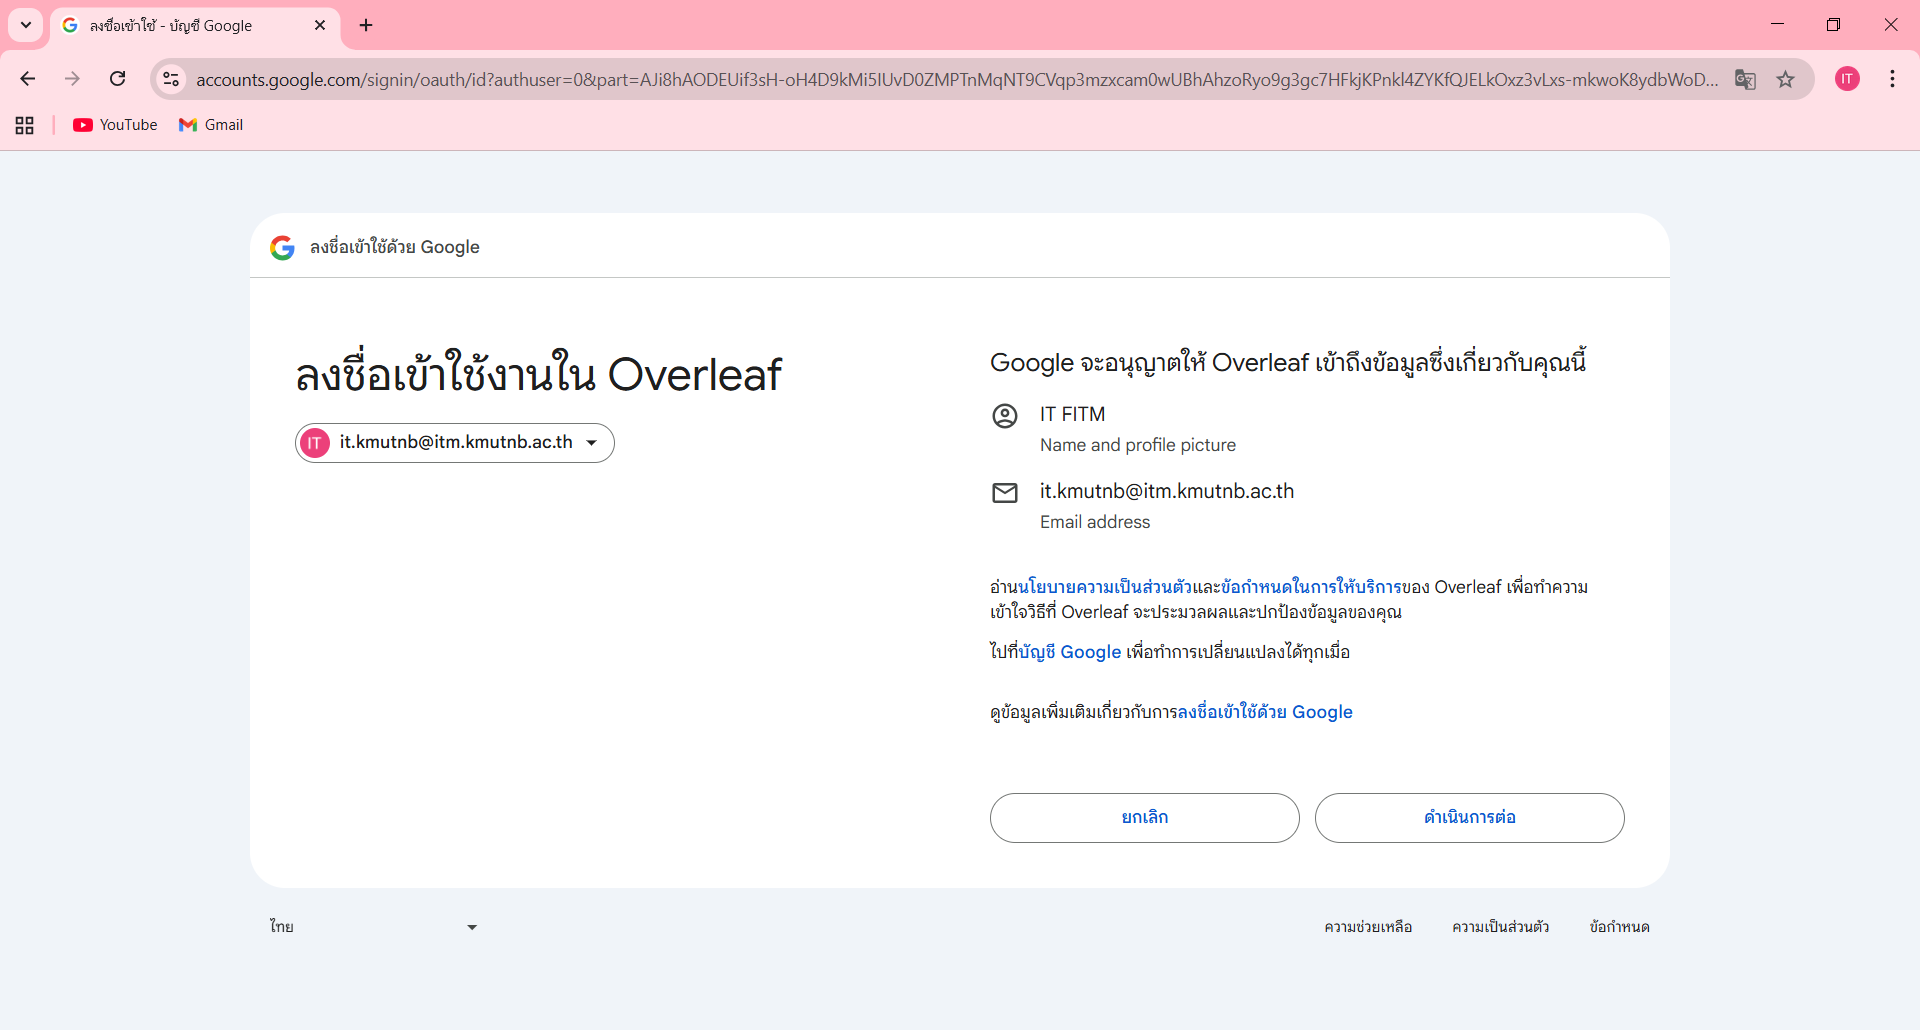
\includegraphics[width=0.8\textwidth]{Image/Overfeaf-4.png}
}
\caption{\fontSixTeen{หน้ายืนยันให้ Overleaf เข้าถึงข้อมูล}}
\label{figA:WebSiteOverleaf4}
\end{figure}

            \item คลิกที่ \enquote{ดำเนินการต่อ} แสดงดังภาพที่ \ref{figA:WebSiteOverleaf5} และให้คลิกที่ คำว่า \enquote{skip}

\begin{figure}[htbp]
\centering
\adjustbox{frame, width=0.8\textwidth}{
    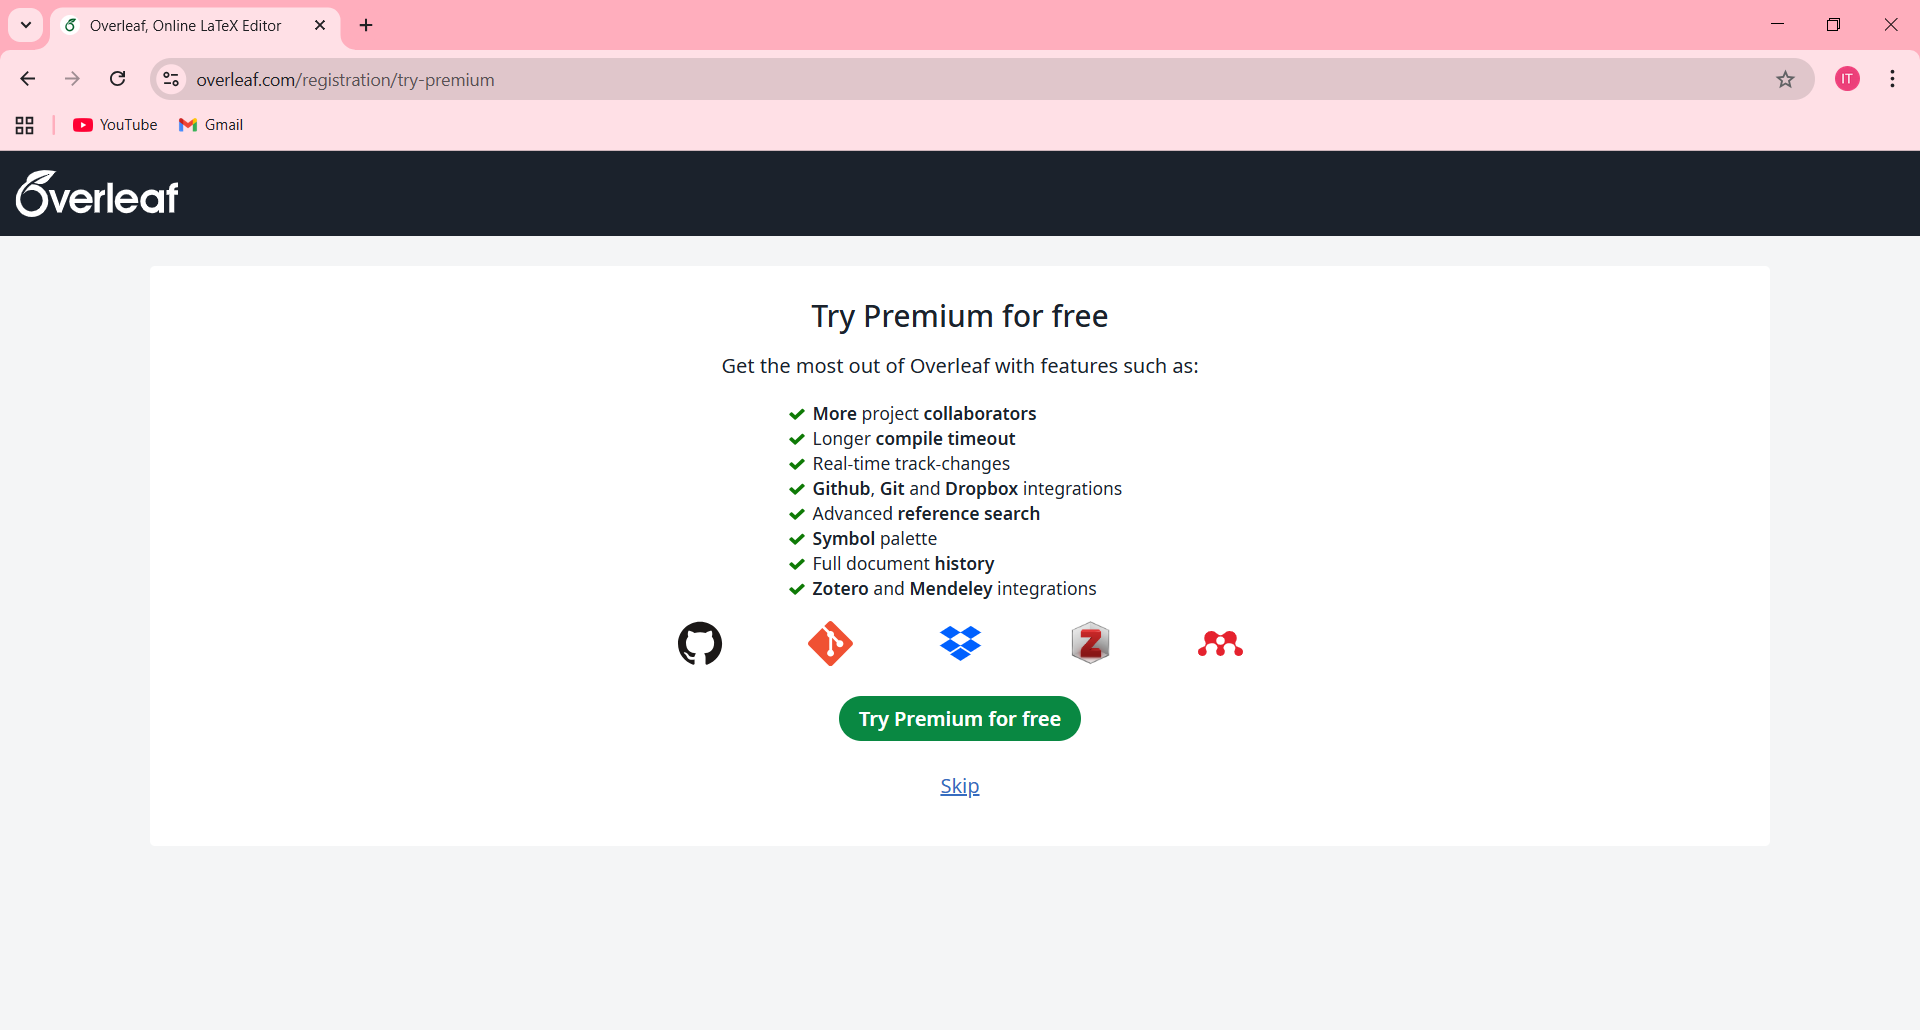
\includegraphics[width=0.8\textwidth]{Image/Overfeaf-5.png}
}
\caption{\fontSixTeen{หน้าเว็บไซต์ Overleaf หลังลงทะเบียน}}
\label{figA:WebSiteOverleaf5}
\end{figure}

            \item ตรวจสอบชื่อและนามสกุลว่าถูกต้องไหม ถ้าชื่อกับนามสกุลถูกต้อง ให้คลิกที่ \enquote{Continue} แสดงดังภาพที่ \ref{figA:WebSiteOverleaf6} \vspace{0.5em}

\begin{figure}[htbp]
\centering
\adjustbox{frame, width=0.8\textwidth}{
    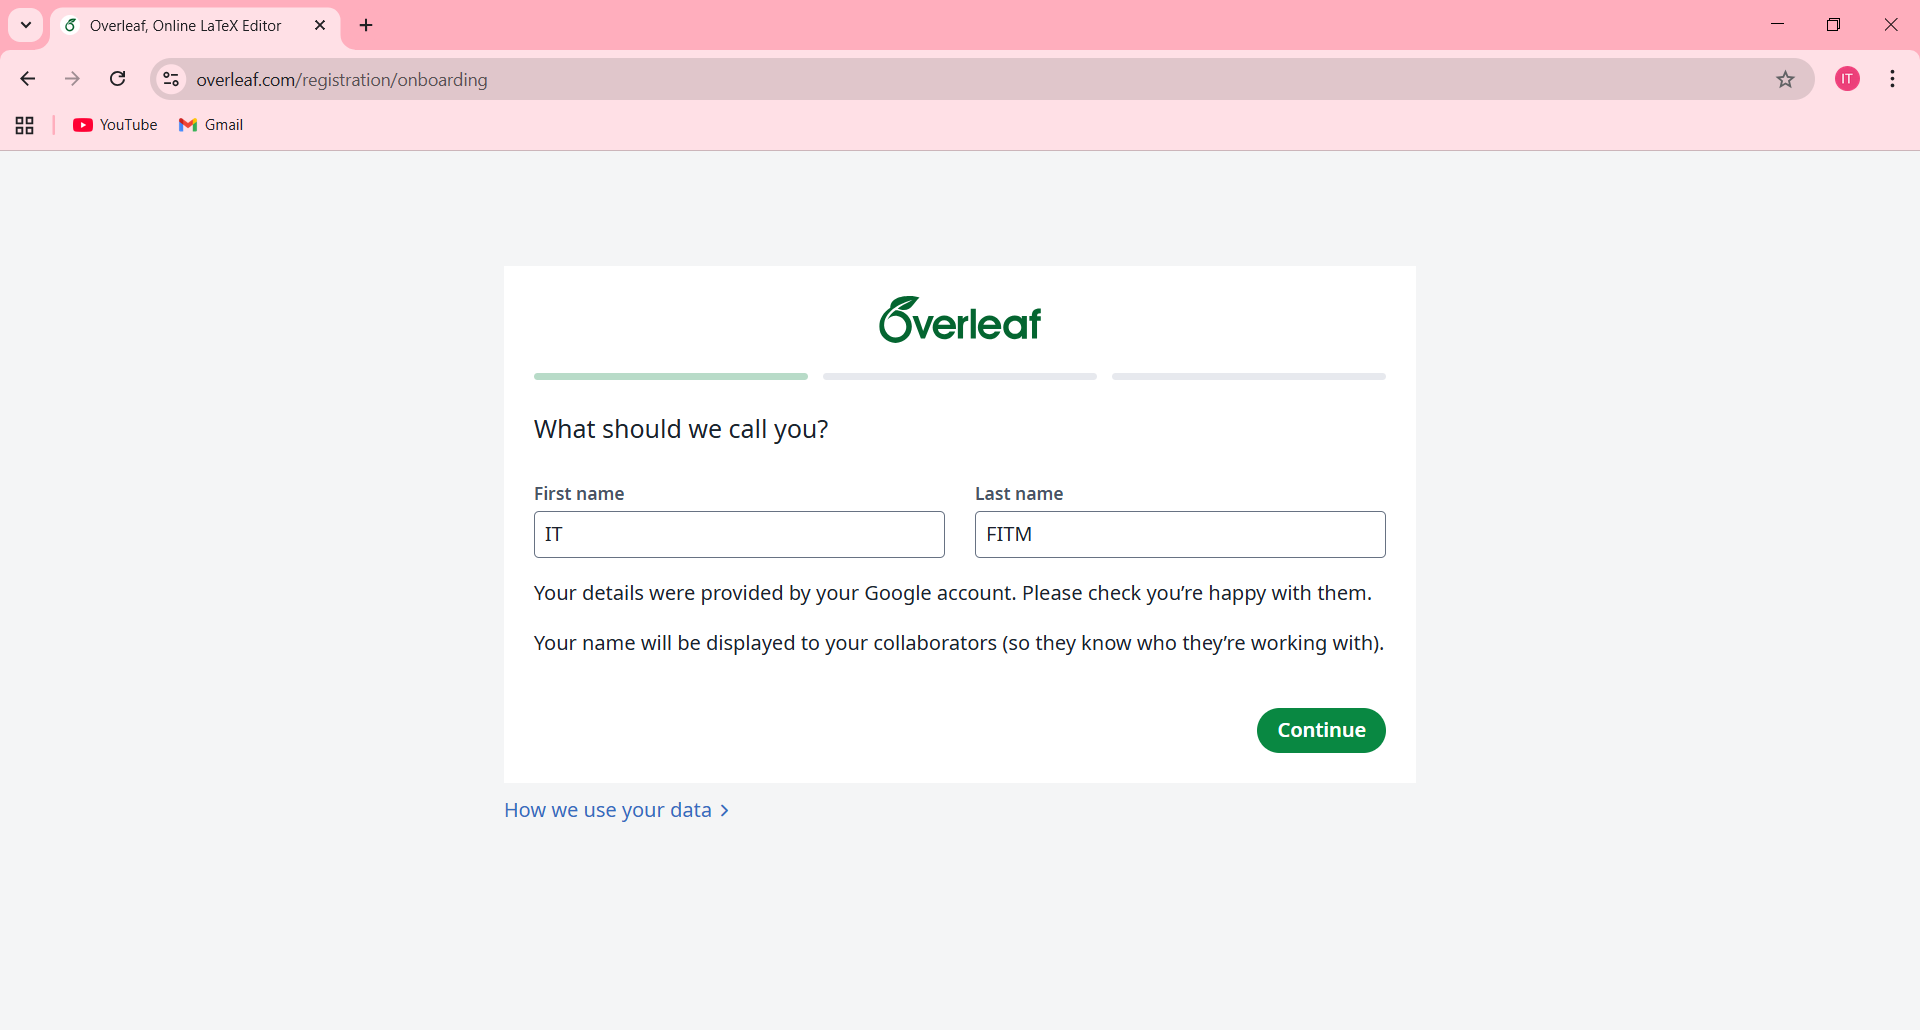
\includegraphics[width=0.8\textwidth]{Image/Overfeaf-6.png}
}
\caption{\fontSixTeen{หน้าตรวจสอบข้อมูลส่วนตัว}}
\label{figA:WebSiteOverleaf6}
\end{figure}

            \item จากนั้นก็ตอบคำถามทั่วไป แล้วคลิกที่ \enquote{Continue} และในหน้าสุดท้ายคลิกที่ \enquote{Go to Overleaf} ก็เป็นอันเสร็จสิ้น แสดงได้ดังภาพที่ \ref{figA:WebSiteOverleaf7} 

\begin{figure}[htbp]
\centering
\adjustbox{frame, width=0.8\textwidth}{
    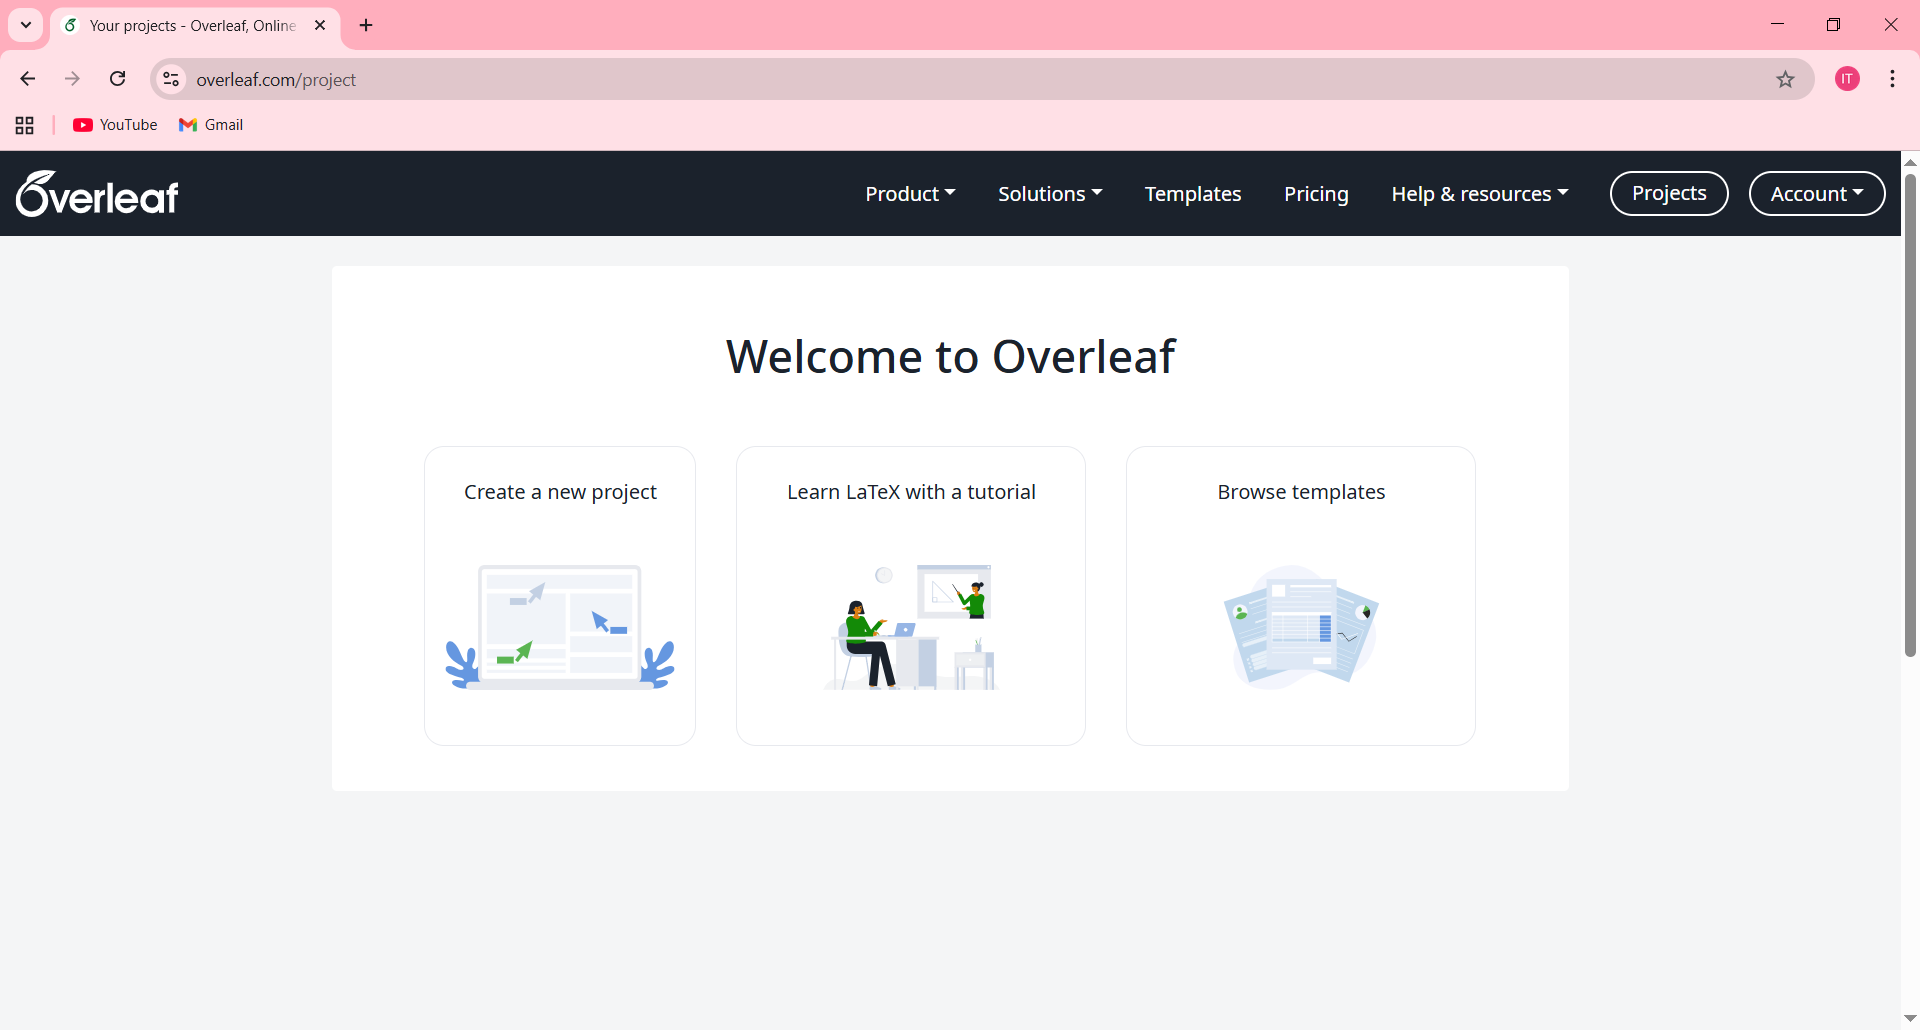
\includegraphics[width=0.8\textwidth]{Image/Overfeaf-7.png}
}
\caption{\fontSixTeen{หน้าแรกหลังจากลงทะเบียนเว็บไซต์ Overleaf สำเร็จแล้ว}}
\label{figA:WebSiteOverleaf7}
\end{figure}
                
        \end{mycustomenum2}   
    \end{mycustomenum2}   
    \item ที่หน้าแรกดังภาพที่ \ref{figA:WebSiteOverleaf1} ในกรณีที่เป็นสมาชิกให้คลิกที่ \enquote{Log in} และเลือก \enquote{Log in with Google} ก็จะพบกับหน้าจอดังภาพที่ \ref{figA:WebSiteOverleaf7}
    
    \item จากภาพที่ \ref{figA:WebSiteOverleaf7} ให้คลิกที่ \enquote{Create a new project} และเลือก \enquote{Upload project} แสดงได้ดังภาพที่ \ref{figA:WebSiteOverleaf8}

\begin{figure}[htbp]
\centering
\adjustbox{frame, width=0.8\textwidth}{
    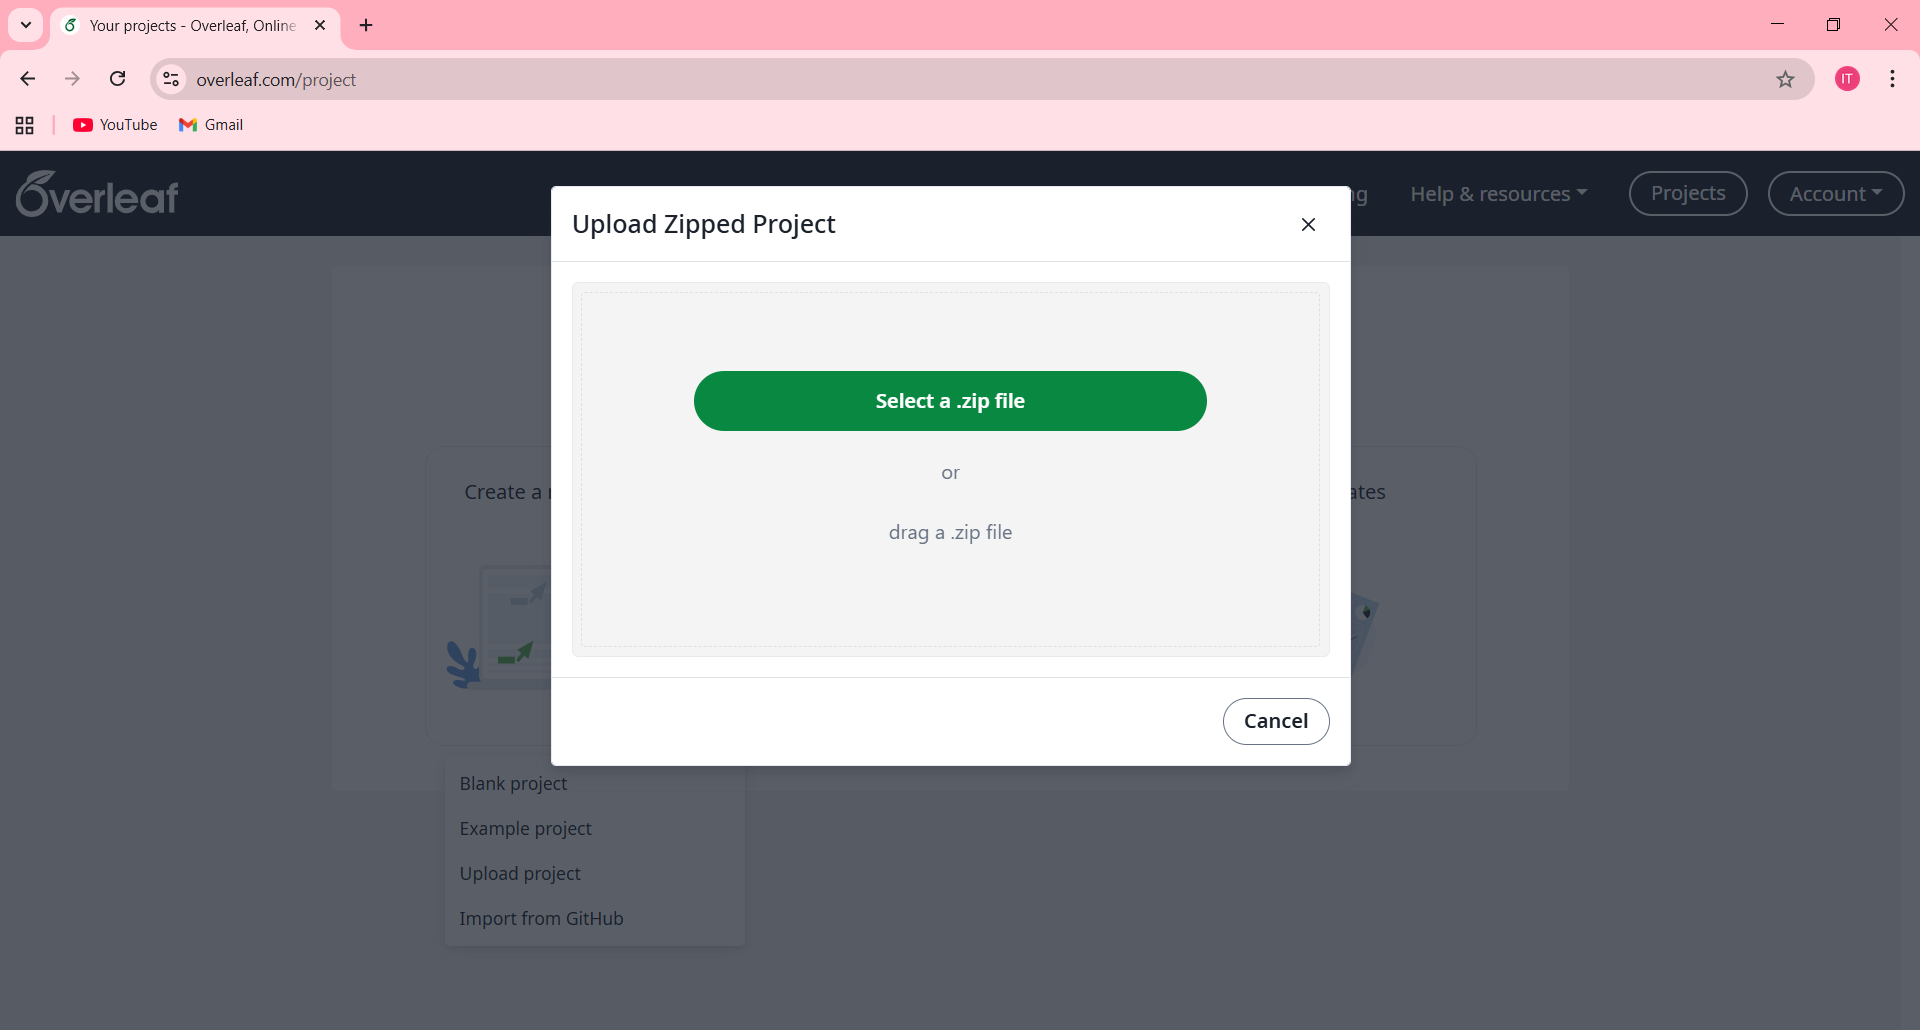
\includegraphics[width=0.8\textwidth]{Image/Overfeaf-8.png}
}
\caption{\fontSixTeen{หน้า Upload a .zip file}}
\label{figA:WebSiteOverleaf8}
\end{figure}

    \item เมื่อคลิกที่ \enquote{Upload a .zip file} และเลือกไฟล์ .zip ที่ upload ได้แล้ว ก็จะแสดงได้ดังภาพที่ \ref{figA:WebSiteOverleaf9}

\begin{figure}[htbp]
\centering
\adjustbox{frame, width=0.8\textwidth}{
    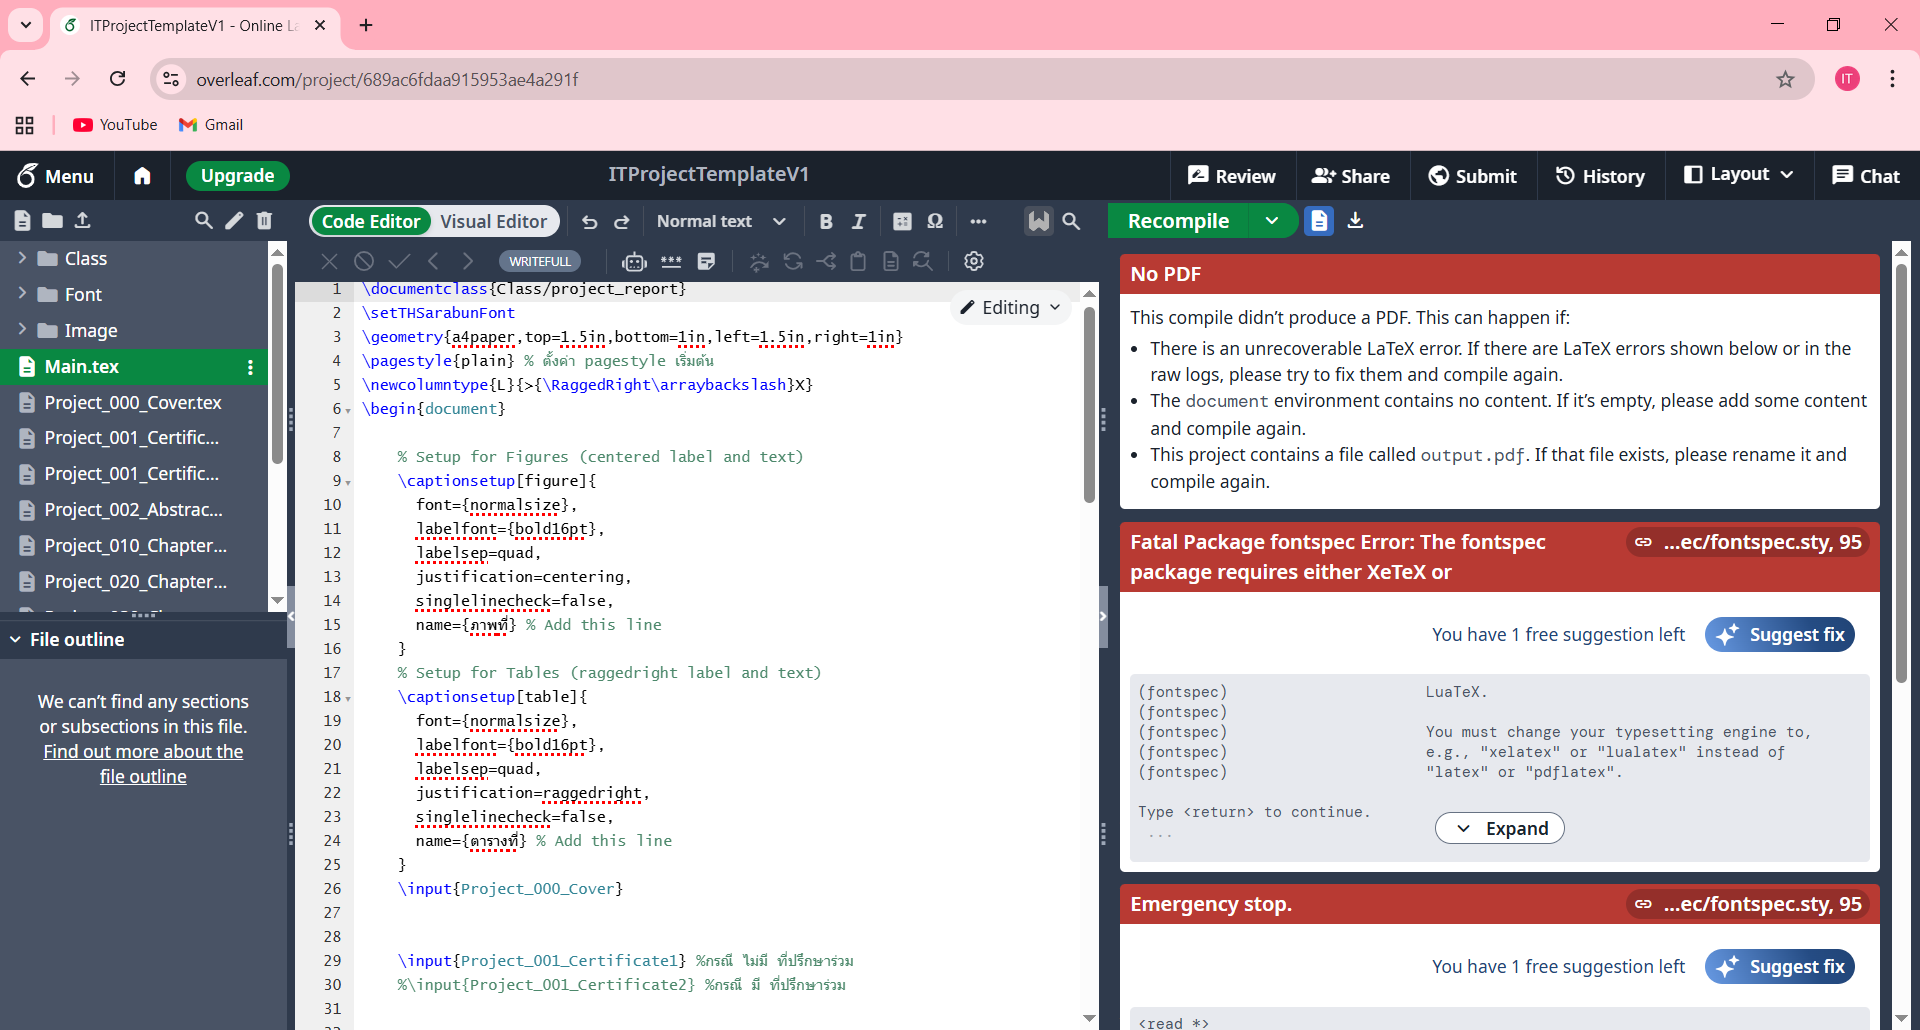
\includegraphics[width=0.8\textwidth]{Image/Overfeaf-9.png}
}
\caption{\fontSixTeen{หน้าสำหรับการแก้ไขเนื้อหาใน Overleaf}}
\label{figA:WebSiteOverleaf9}
\end{figure}

    \item จากภาพที่ \ref{figA:WebSiteOverleaf9} ให้คลิกที่ \enquote{Menu} ที่อยู่มุมซ้ายบน และที่ Compiler ให้เปลี่ยนเป็น \enquote{XeLaTex} และ Spell check ให้เป็น \enquote{Thai} ดังภาพที่ \ref{figA:WebSiteOverleaf10} 

\begin{figure}[htbp]
\centering
\adjustbox{frame, width=0.8\textwidth}{
    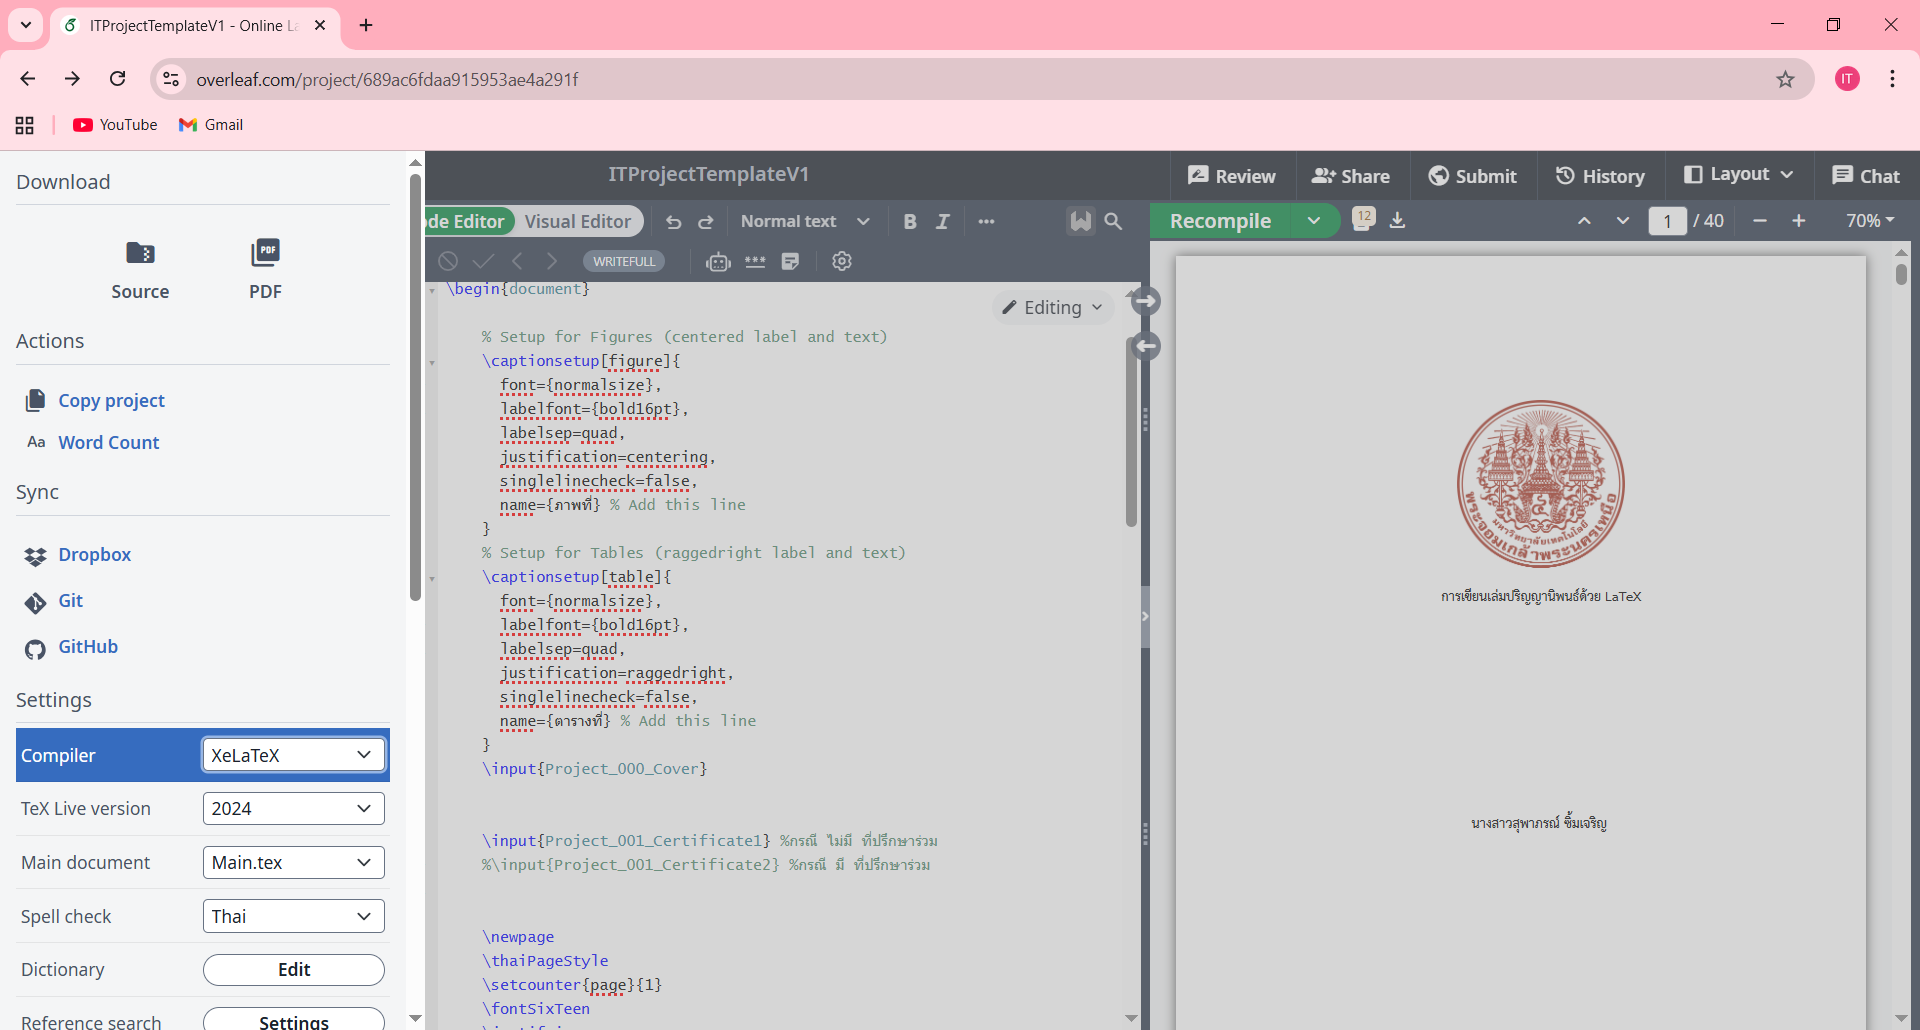
\includegraphics[width=0.8\textwidth]{Image/Overfeaf-10.png}
}
\caption{\fontSixTeen{หน้าสำหรับเปลี่ยน Compiler และ Spell check}}
\label{figA:WebSiteOverleaf10}
\end{figure}

    \item เมื่อคลิกที่ \enquote{Recompile} Error ก็จะหายไป แสดงได้ดังภาพที่  \ref{figA:WebSiteOverleaf11}

\begin{figure}[htbp]
\centering
\adjustbox{frame, width=0.8\textwidth}{
    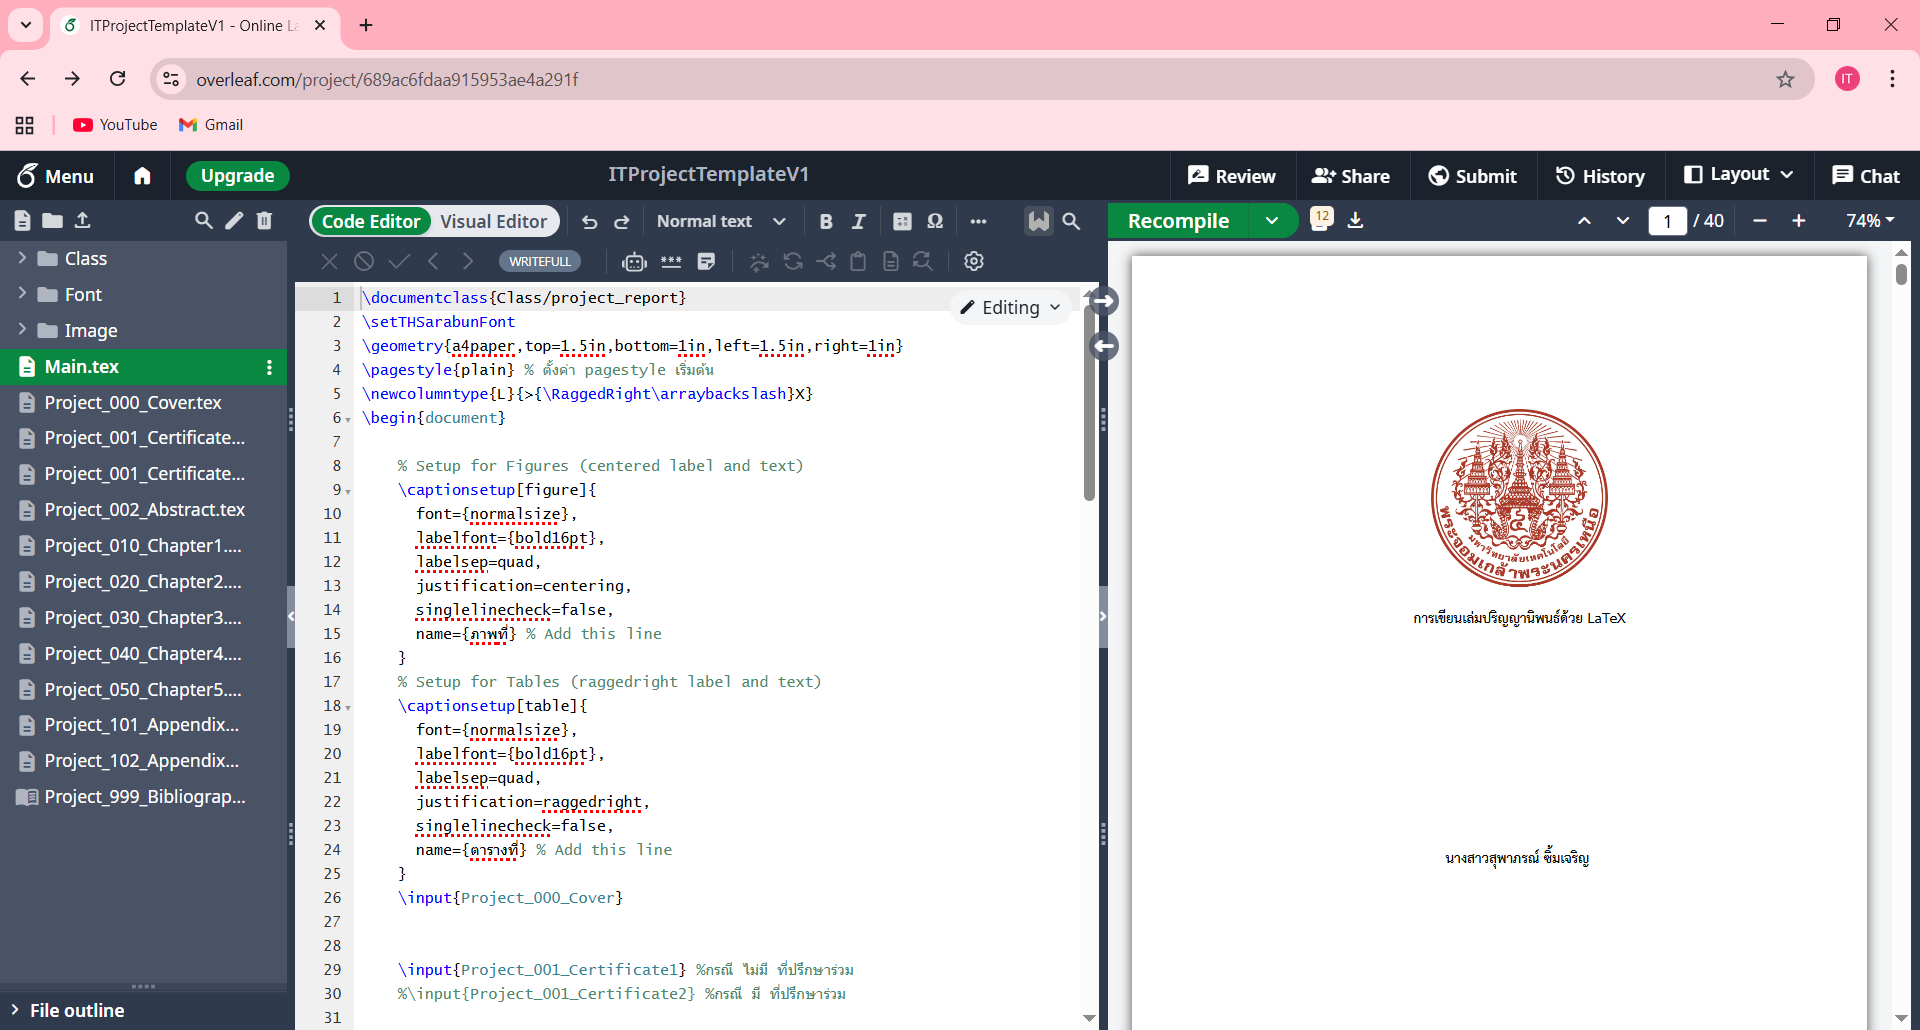
\includegraphics[width=0.8\textwidth]{Image/Overfeaf-11.png}
}
\caption{\fontSixTeen{หน้าหลังจากที่เปลี่ยน Compile เป็น "XeLaTex"}}
\label{figA:WebSiteOverleaf11}
\end{figure}

    \item เมื่อต้องการกลับหน้ารวม Project ให้คลิกที่ icon \enquote{รูปบ้าน} ที่มุมบนซ้าย ก็จะไปยังหน้า Home ที่รวมโปรเจ็คทั้งหมด แสดงได้ดังภาพที่ \ref{figA:WebSiteOverleaf12}

\begin{figure}[htbp]
\centering
\adjustbox{frame, width=0.8\textwidth}{
    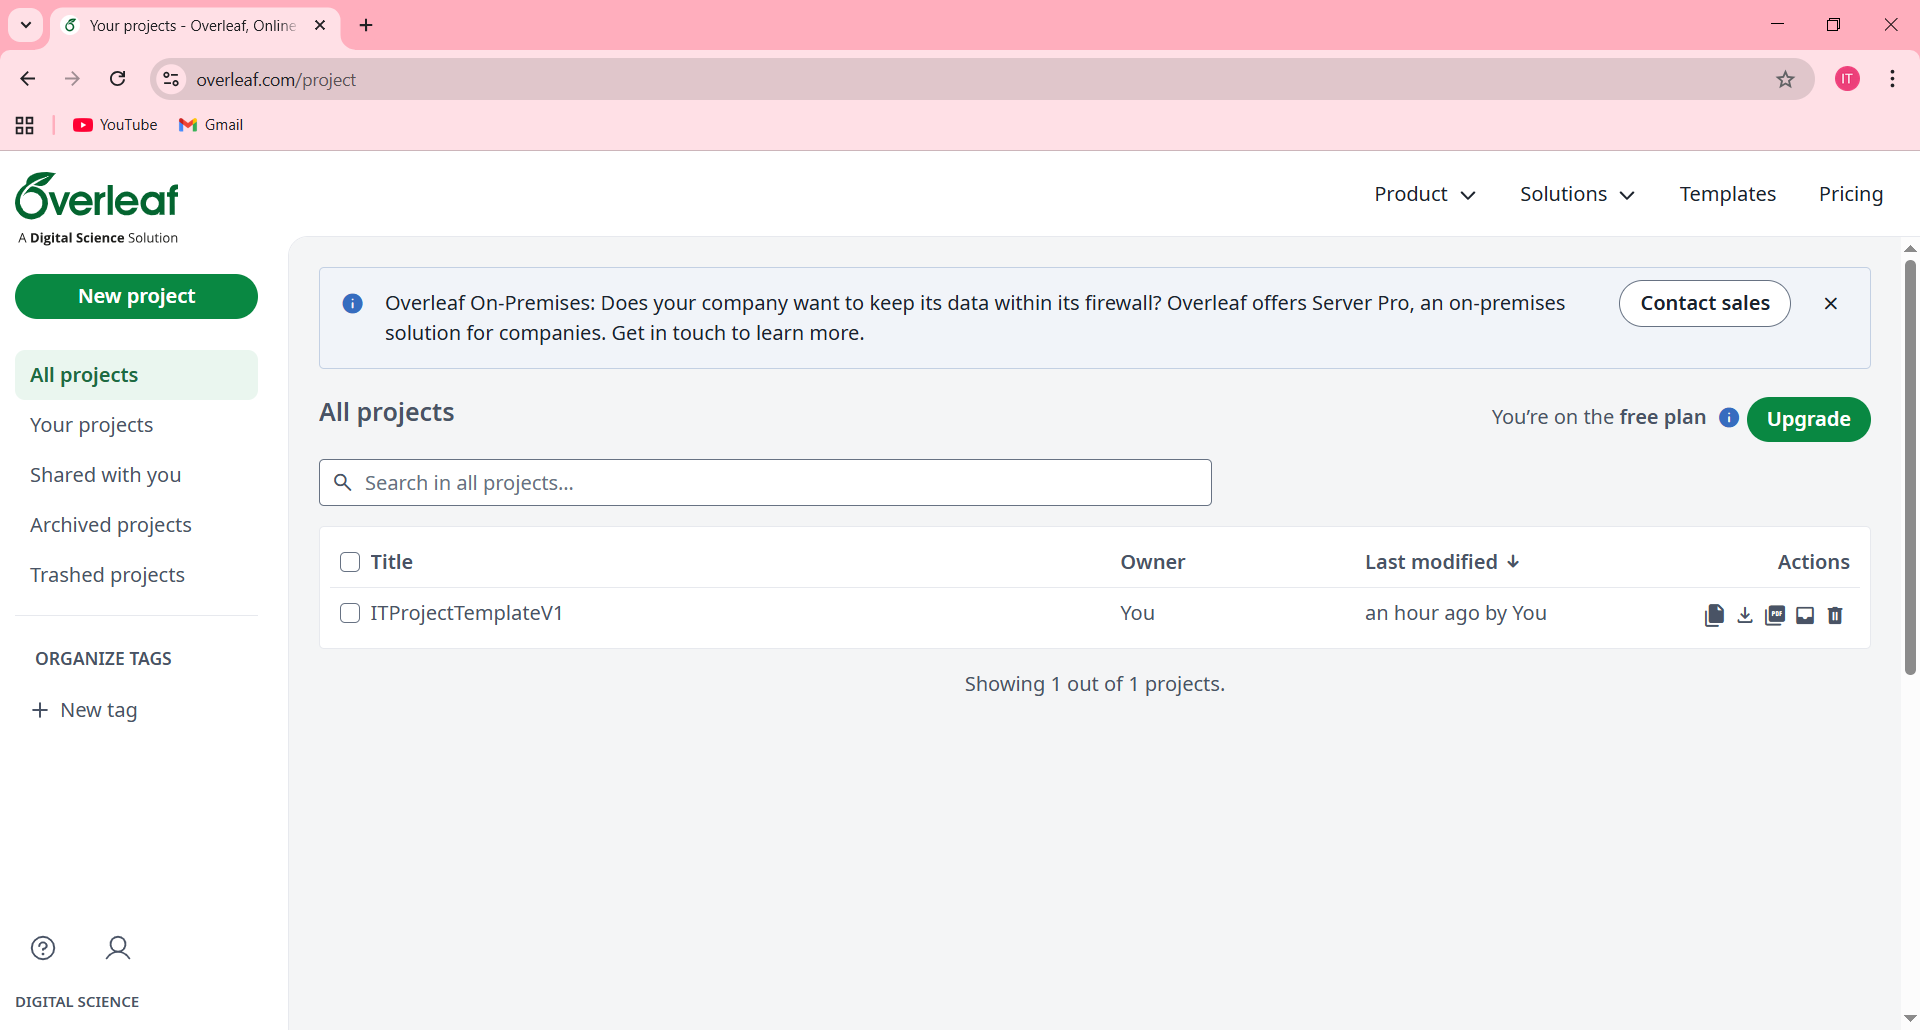
\includegraphics[width=0.8\textwidth]{Image/Overfeaf-12.png}
}
\caption{\fontSixTeen{หน้าสำหรับเปลี่ยน Compiler}}
\label{figA:WebSiteOverleaf12}
\end{figure}

\end{mycustomenum2}

    %*************************************
% ภาคผนวก ข.
%*************************************
\appendixChapterTitle{ข}{การเพิ่มไฟล์ภาคผนวก}
\section{การเพิ่มไฟล์ภาคผนวก}
\hspace*{1.5em}
ตัวอย่างการเพิ่มไฟล์ภาคผนวก เมื่อต้องการเพิ่มภาคผนวก ค. มีรายละเอียดดังนี้
\vspace{0.5em}

\begin{mycustomenum2}
    \item คลิกที่ icon \enquote{New file} ที่มุมบนซ้าย จากนั้นให้ตั้งชื่อไฟล์ ดังภาพที่  \ref{figB:CreateFile1}

\begin{figure}[htbp]
\centering
\adjustbox{frame, width=0.8\textwidth}{
    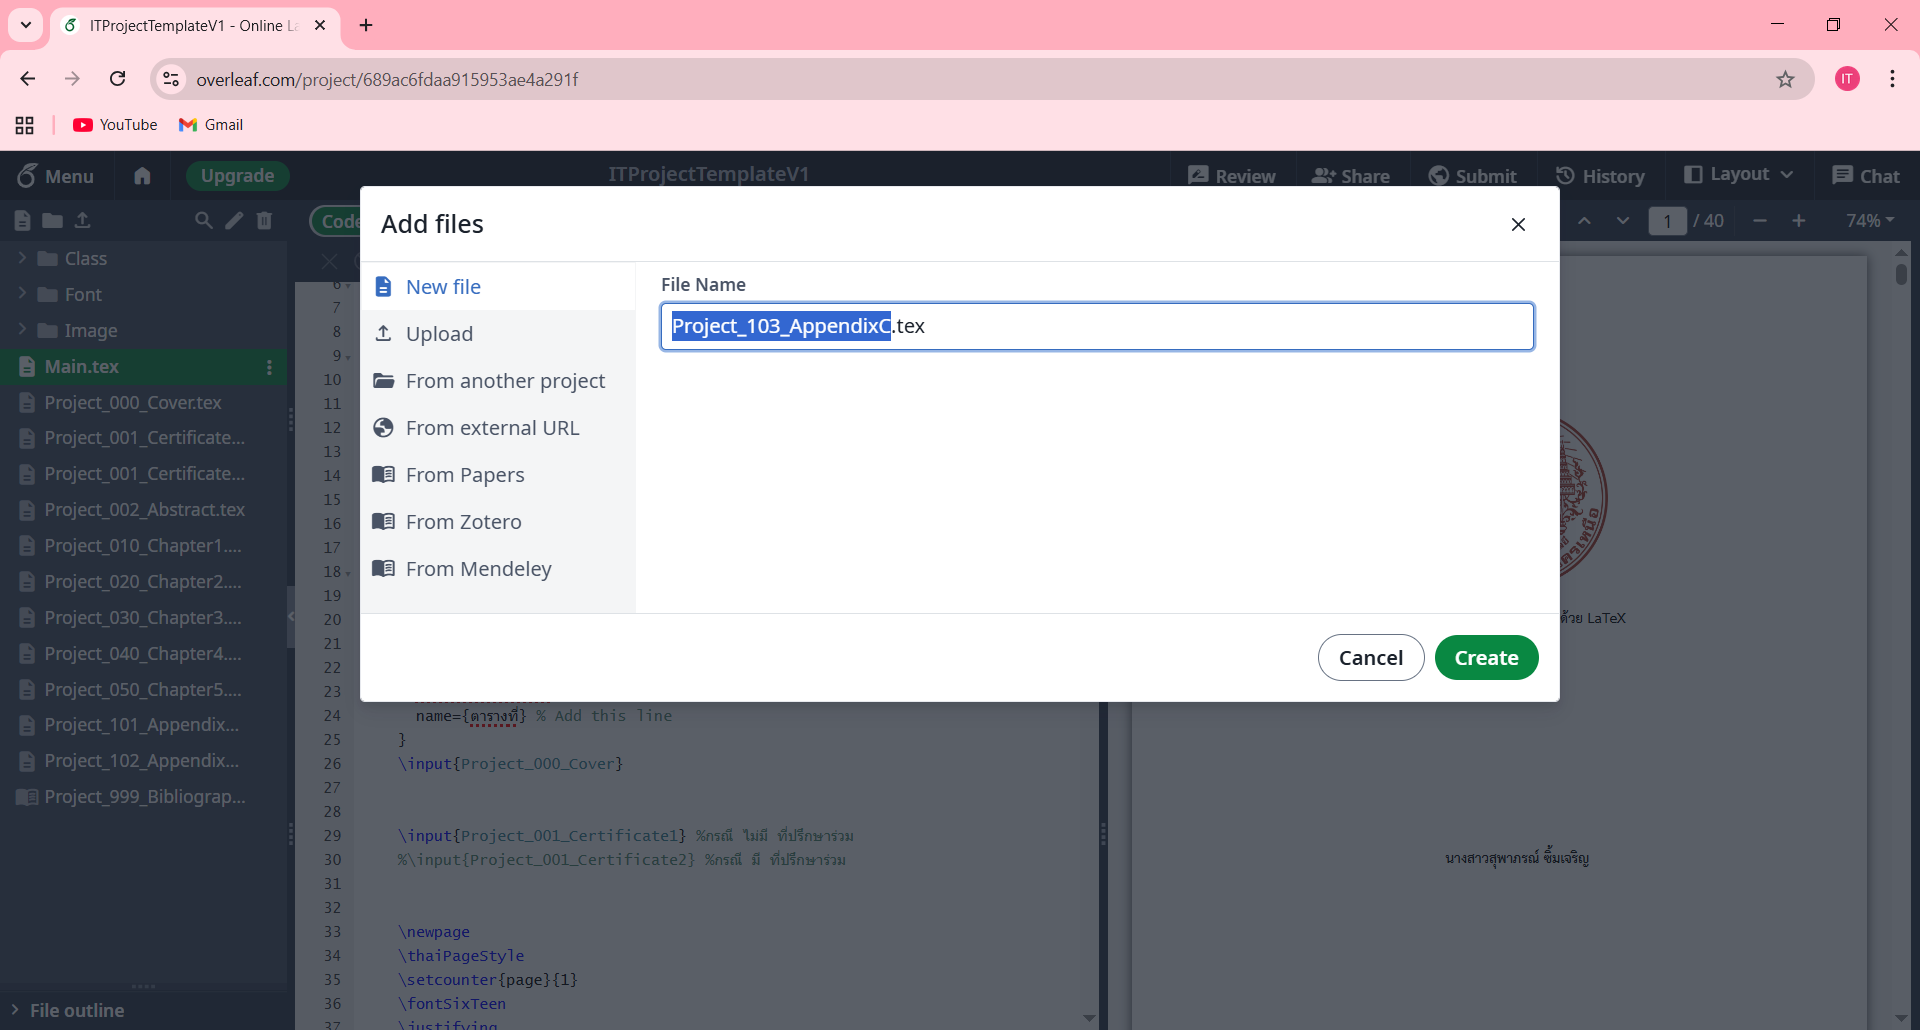
\includegraphics[width=0.8\textwidth]{Image/CreateFile-1.png}
}
\caption{\fontSixTeen{ตั้งชื่อไฟล์ .tex}}
\label{figB:CreateFile1}
\end{figure}

    \item เมื่อคลิกที่ \enquote{Create} ก็สามารถเพิ่มเนื้อหาของภาคผนวก ค. ลงไปได้เลย ดังภาพที่ \ref{figB:CreateFile2}

\begin{figure}[htbp]
\centering
\adjustbox{frame, width=0.8\textwidth}{
    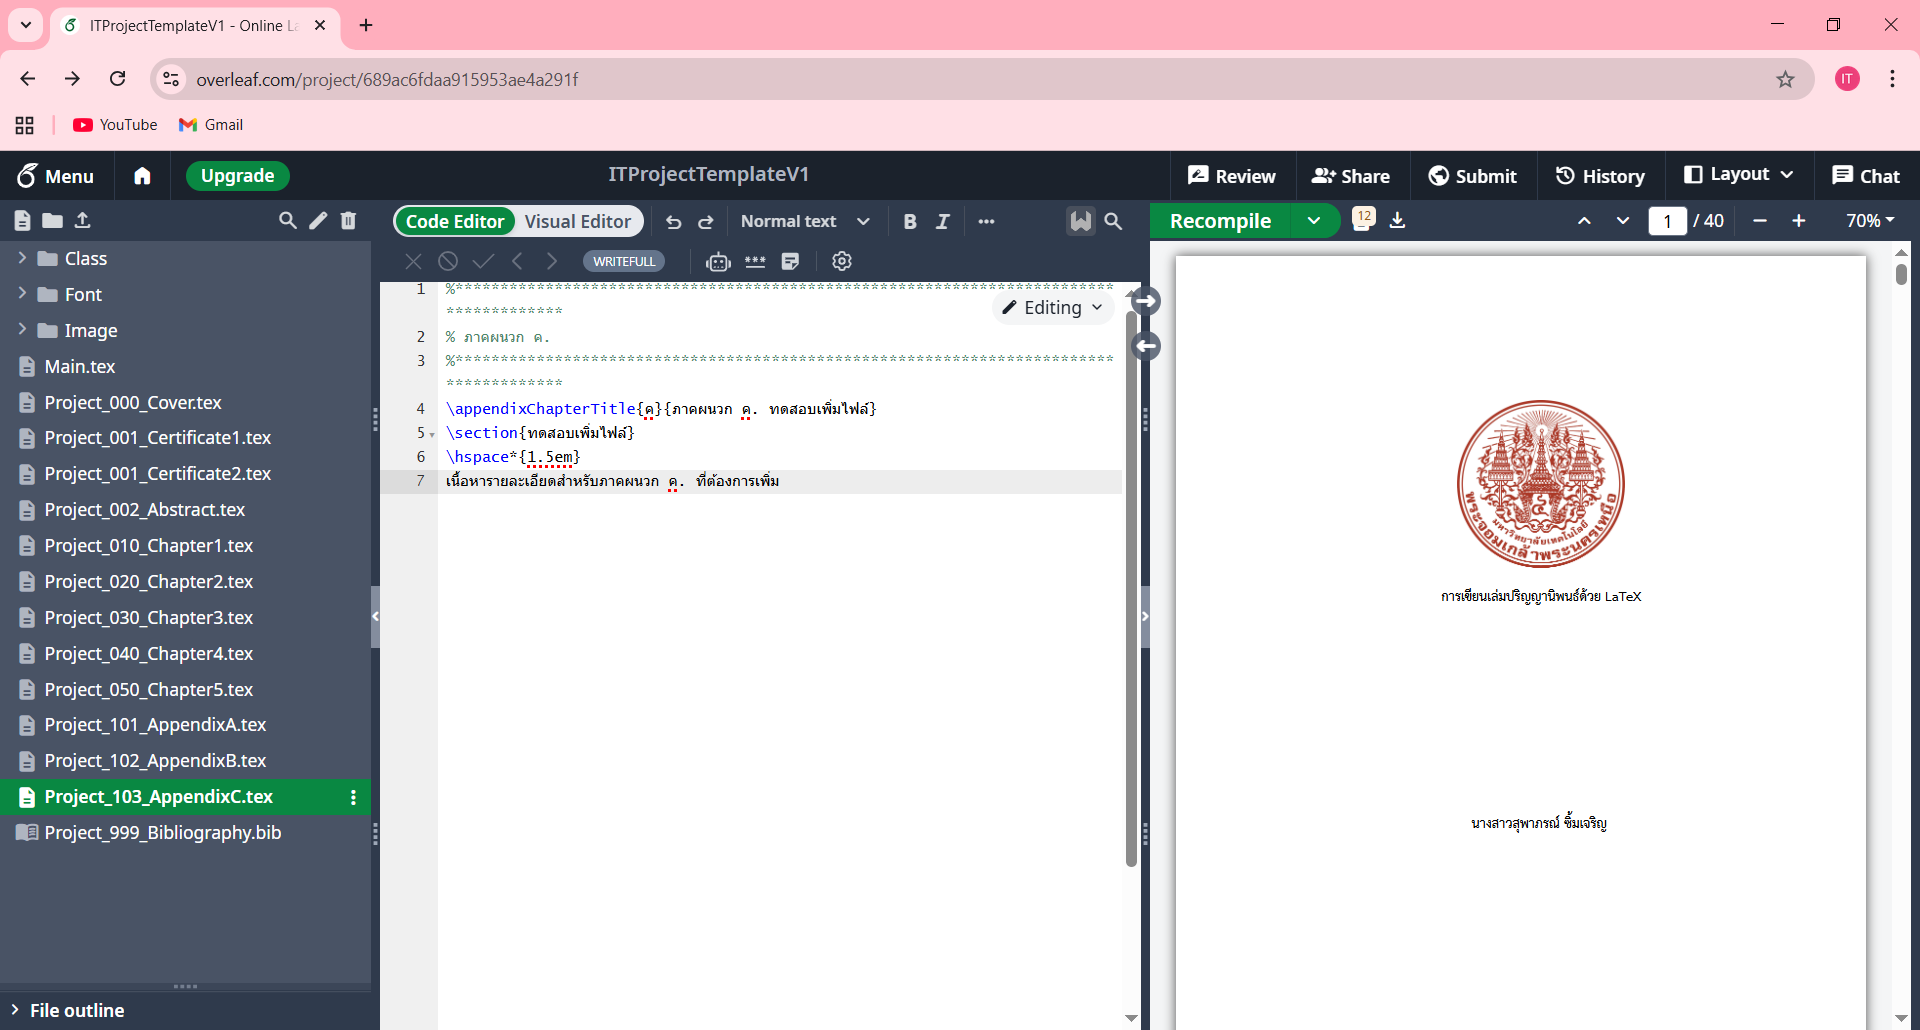
\includegraphics[width=0.8\textwidth]{Image/CreateFile-2.png}
}
\caption{\fontSixTeen{เพิ่มเนื้อหาลงไปในไฟล์ .tex}}
\label{figB:CreateFile2}
\end{figure}

    \item จากนั้นให้ไปเพิ่มโค้ดการเรียกไฟล์ใหม่ที่สร้างขึ้น ที่ไฟล์ Main.tex ดังภาพที่ \ref{figB:CreateFile3}

\begin{figure}[htbp]
\centering
\adjustbox{frame, width=0.8\textwidth}{
    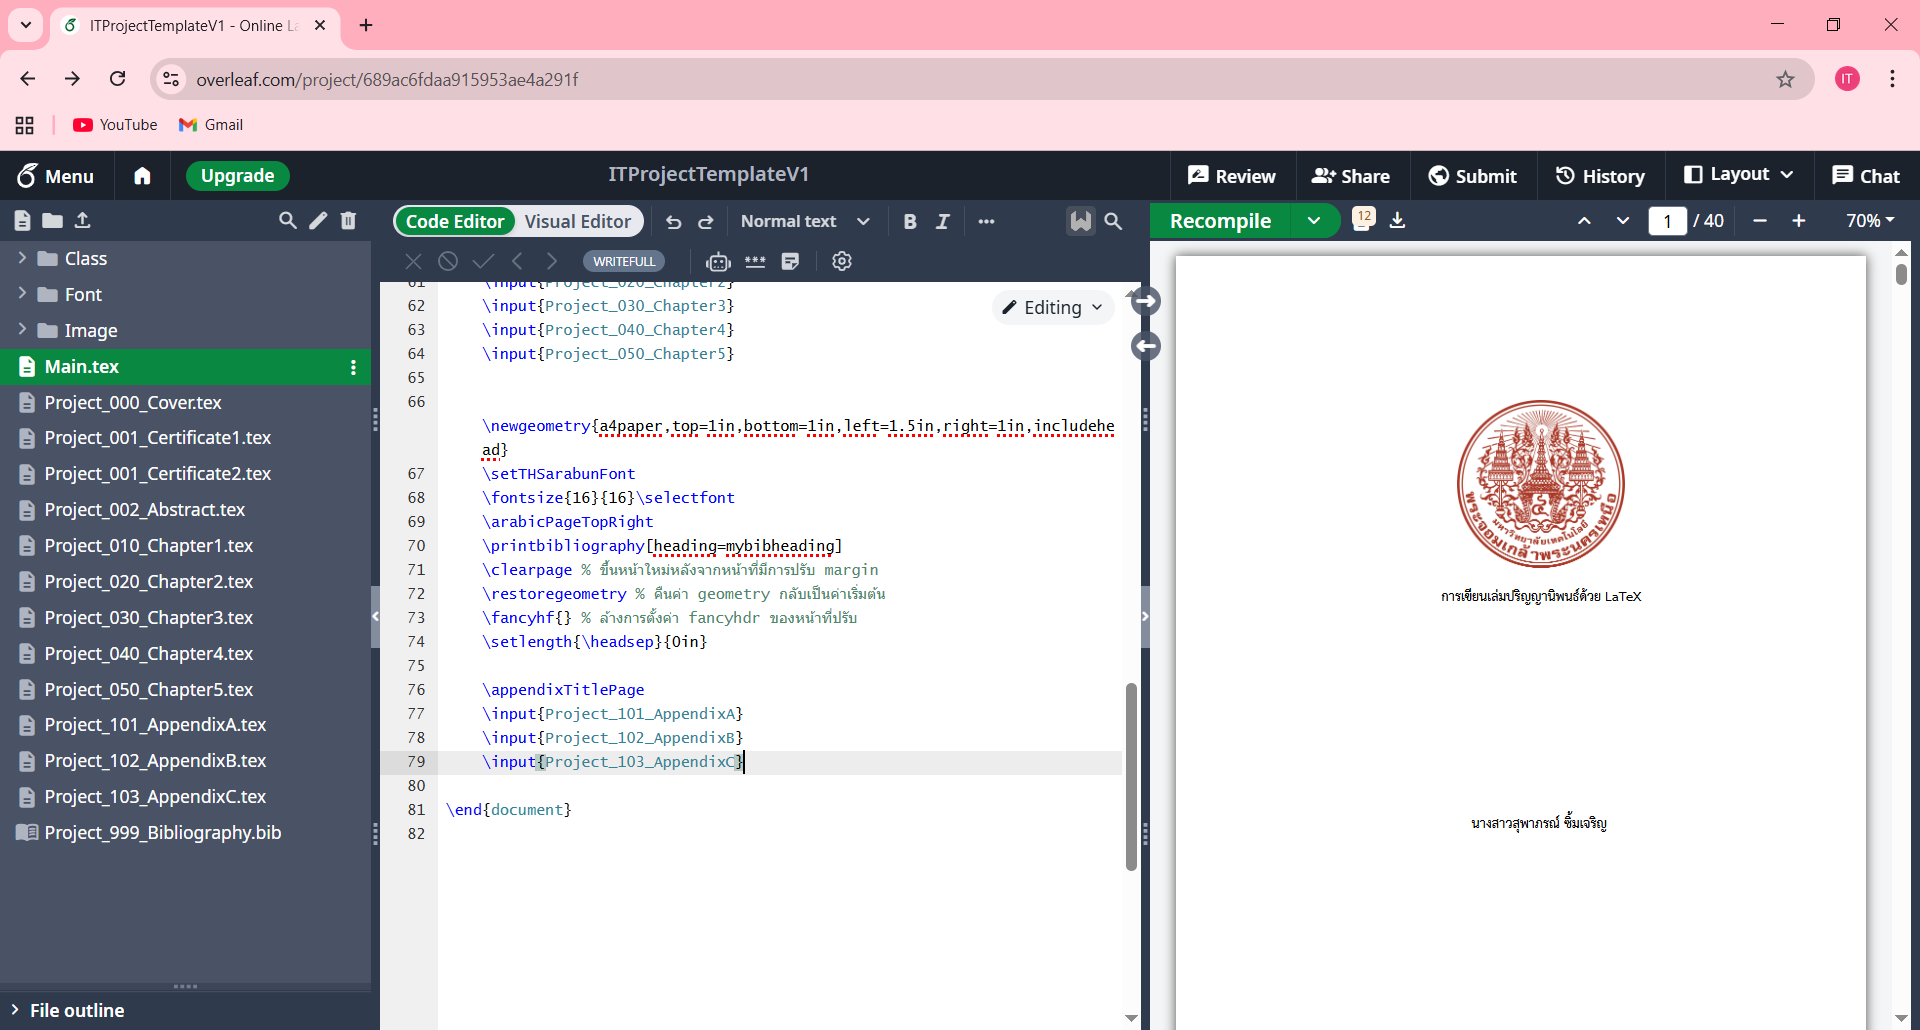
\includegraphics[width=0.8\textwidth]{Image/CreateFile-3.png}
}
\caption{\fontSixTeen{เพิ่มโค้ดสำหรับเรียกไฟล์ .tex ที่สร้างใหม่}}
\label{figB:CreateFile3}
\end{figure}

    \item จากนั้นคลิกที่ Recompile ภาคผนวก ค. ก็จะสามารถใช้งานได้ ดังภาพที่ \ref{figB:CreateFile4}

\begin{figure}[htbp]
\centering
\adjustbox{frame, width=0.8\textwidth}{
    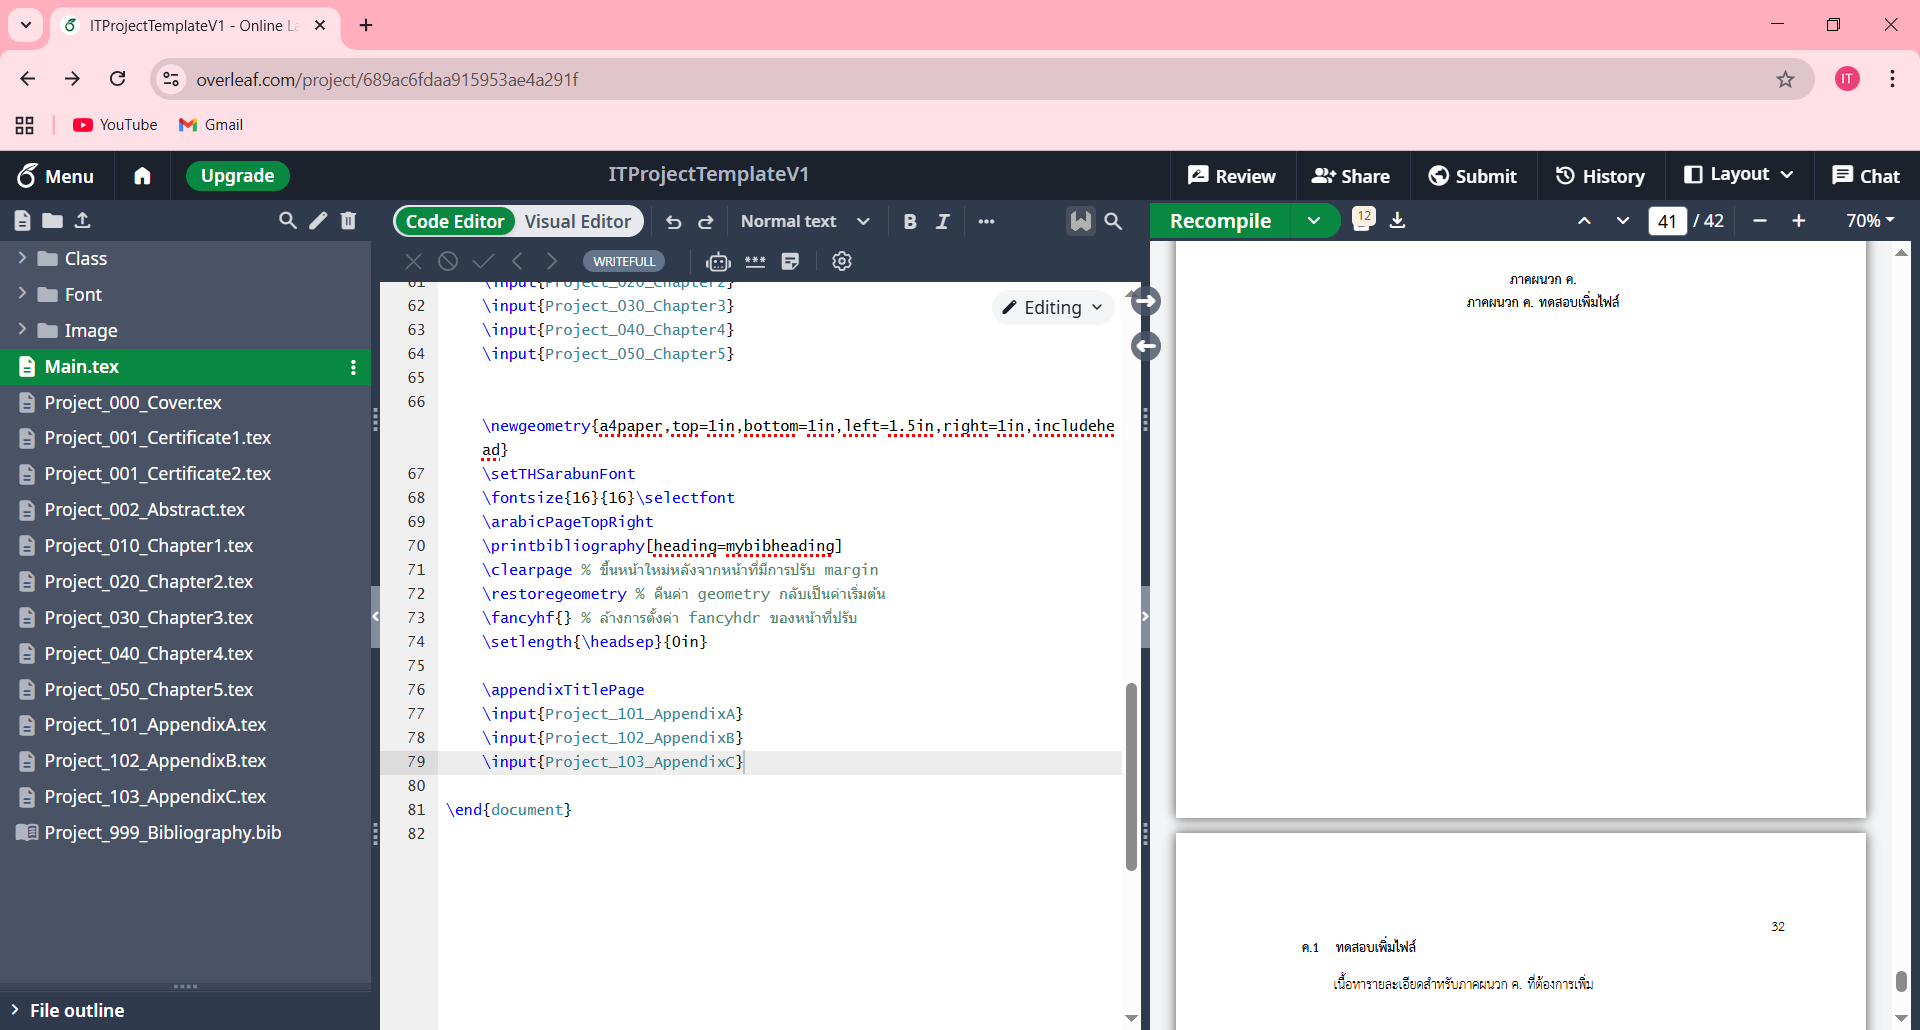
\includegraphics[width=0.8\textwidth]{Image/CreateFile-4.png}
}
\caption{\fontSixTeen{ภาคผนวก ค. แสดงหลังจาก Recompile}}
\label{figB:CreateFile4}
\end{figure}

    \item ในกรณีที่ไม่ต้องการให้เนื้อหาของไฟล์ใดปรากฏ ก็สามารถ Comment ที่โค้ดบรรทัดของการเรียกไฟล์ได้ที่ไฟล์ Main.tex ตัวอย่างการ Comment แสดงได้ดังภาพที่ \ref{figB:CreateFile5} 

\begin{figure}[htbp]
\centering
\adjustbox{frame, width=0.8\textwidth}{
    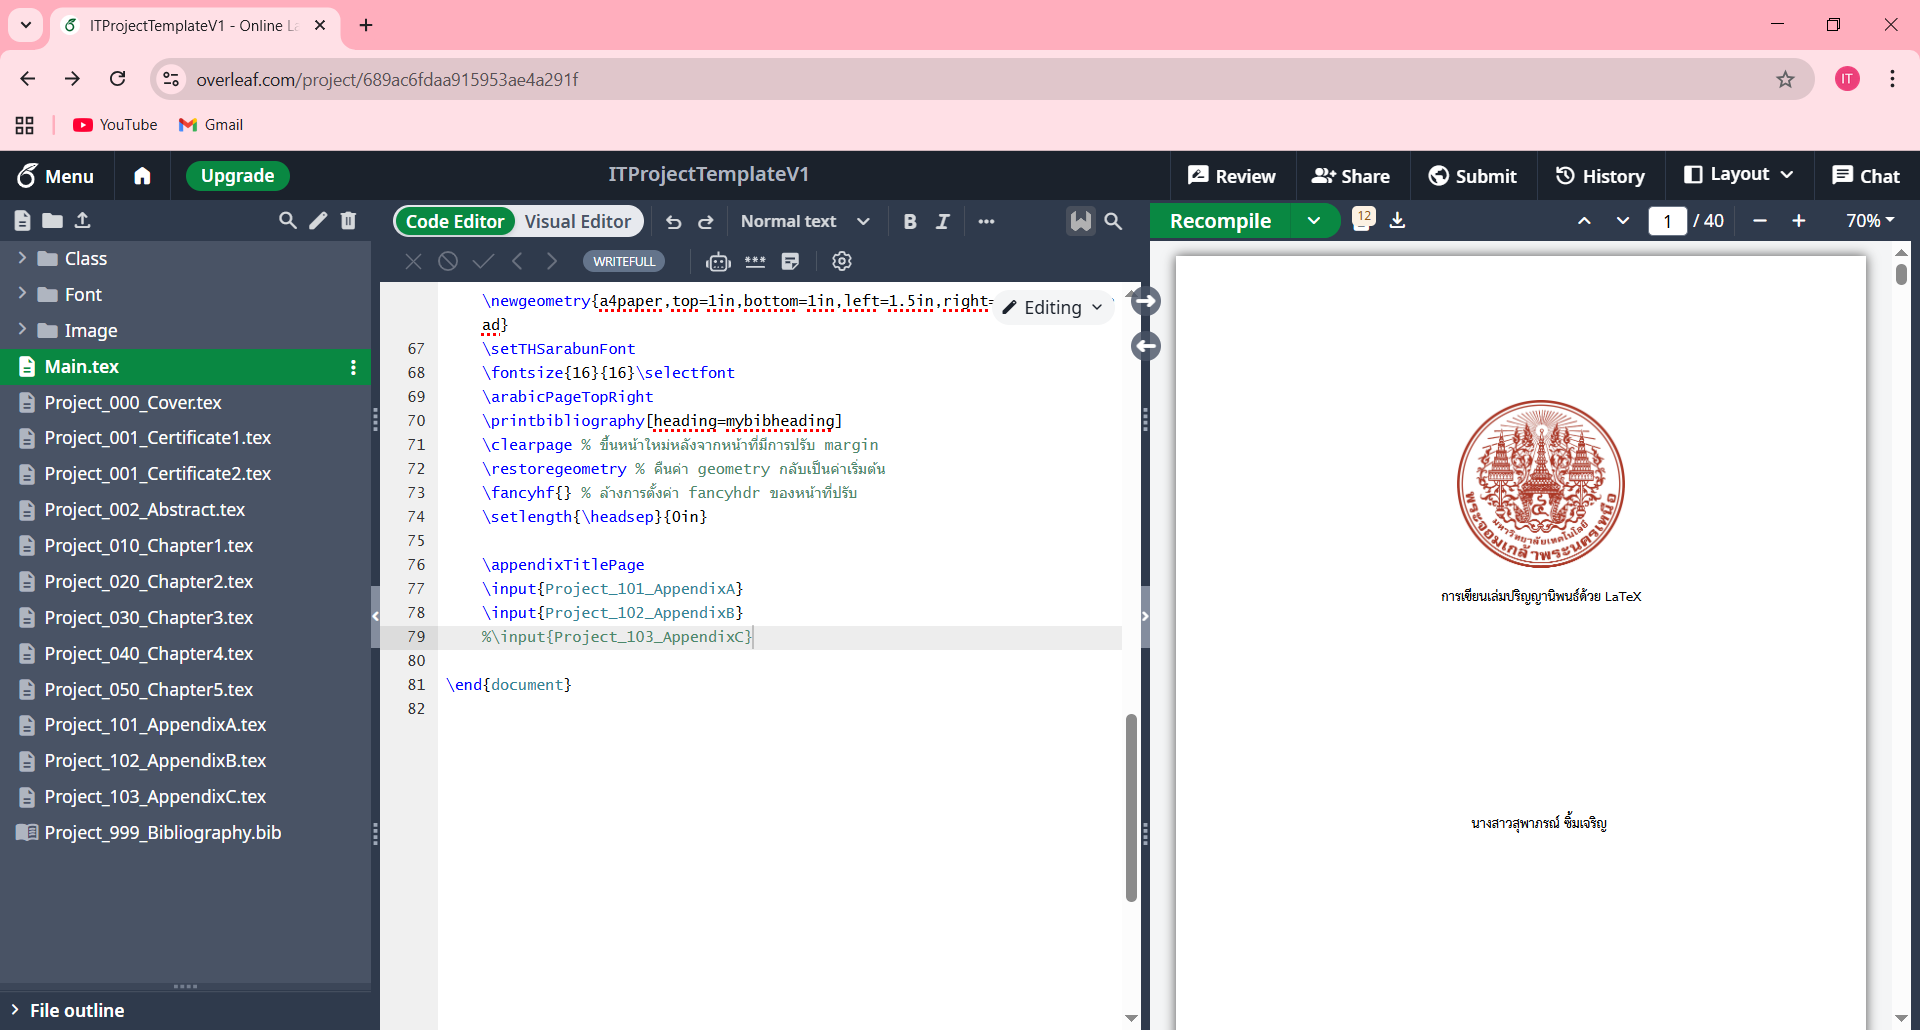
\includegraphics[width=0.8\textwidth]{Image/CreateFile-5.png}
}
\caption{\fontSixTeen{ตัวอย่างการ Comment ไฟล์ .tex ที่ไม่ต้องการแสดง}}
\label{figB:CreateFile5}
\end{figure}

\end{mycustomenum2}

\end{document}
